%% ========================================================================
%%%% Basic settings
%% ========================================================================
%% (idea of using newcommands for basic documentclass settings from: Thomas Schlager)

\newcommand{\mypapersize}{A4}
%% e.g., "A4", "letter", "legal", "executive", ...
%% The size of the paper of the resulting PDF file.

\newcommand{\mylaterality}{oneside}
%% "oneside" or "twoside"
%% Either you are creating a document which is printed on both, left pages
%% and right pages (twoside) or you create a document which is printed
%% on right pages only (oneside).

\newcommand{\mydraft}{false}
%% "true" or "false"
%% Use draft mode? If true, included graphics are replaced by empty
%% rectangles (of same size) and overfull boxes (in margin space) are
%% marked with black box (-> easy to spot!)

\newcommand{\myparskip}{half}
%% e.g., "no", "full", "half", ...
%% How to separate paragraphs: indention ("no") or spacing ("half",
%% "full", ...).

\newcommand{\myBCOR}{0mm}
%% Inner binding correction. This value depends on the method which is
%% being used to bind your printed result. Some techniques do not
%% require a binding correction at all ("0mm"), other require for
%% example "5mm". Refer to KOMA script documentation for a detailed
%% explanation what a binding correction is and how to measure it.

\newcommand{\myfontsize}{12pt}
%% e.g., 10pt, 11pt, 12pt
%% The font size of the main text in pt (points).

\newcommand{\mylinespread}{1.0}
%% e.g., 1.0, 1.5, 2.0
%% Line spacing in %/100. For example 1.5 means 150% of the usual line
%% spacing. Please use with caution: 100% ("1.0") is fine because the
%% font was designed for it.

\newcommand{\mylanguage}{american,ngerman}
%% "english,ngerman", "ngerman,english", ...
%% NOTE: The *last* language is the active one!
%% See babel documentation for further details.

%% BibLaTeX-settings: (see biblatex reference for further description)
\newcommand{\mybiblatexstyle}{numeric}
%% e.g., "alphabetic", "authoryear", ...
%% The biblatex style which is being used for referencing. See
%% biblatex documentation for further details and more values.
%%
%% CAUTION: if you change the style, please check for (in)compatible
%%          "biblatex" package options in the file
%%          "template/preamble.tex"! For example: "alphabetic" does
%%          not have an option "dashed=..." and causes an error if it
%%          does not get removed from the list of options.

\newcommand{\mybiblatexdashed}{false}  %% "true" or "false"
%% If true: replace recurring reference authors with a dash.

\newcommand{\mybiblatexbackref}{true}  %% "true" or "false"
%% If true: create backward links from reference to citations.

\newcommand{\mybiblatexfile}{references-biblatex.bib}
%% Name of the biblatex file that holds the references.

%\newcommand{\mydispositioncolor}{30,103,182}
\newcommand{\mydispositioncolor}{0,0,0}
%% e.g., "30,103,182" (blue/turquois), "0,0,0" (black), ...
%% Color of the headings and so forth in RGB (red,green,blue) values.
%% NOTE: if you are using "0,0,0" for black, printers might still
%%       recognize pages as color pages. In case this is a problem
%%       (paying for color print-outs vs. paying for b/w-printouts)
%%       please edit file "template/preamble.tex" and change
%%       "\definecolor{DispositionColor}{RGB}{\mydispositioncolor}"
%%       to "\definecolor{DispositionColor}{gray}{0}" and thus
%%       overwriting the value of \mydispositioncolor above.

\newcommand{\mycolorlinks}{true}  %% "true" or "false"
%% Enables or disables colored links (hyperref package).

\newcommand{\mytitlepage}{template/title_VWA}
%% Your own or one of following pre-defined title pages:
%% "template/title_plain_maketitle": simple maketitle page
%% "template/title_Diplomarbeit_KF_Uni_Graz.tex": fancy (german) title page for KF Uni Graz
%% "template/title_Thesis_TU_Graz":
%%             titlepage for Graz University of Technology (correct
%%             (old?) Corporate Design) by Karl Voit (2012)
%% "template/title_Thesis_TU_Graz_-_kazemakase":
%%             titlepage for Graz University of Technology
%%             (correct new Corporate Design) by kazemakase (2013):
%%             see https://github.com/novoid/LaTeX-KOMA-template/issues/5
%% "template/title_VWA": titlepage for Vorwissenschaftliche Arbeit

\newcommand{\mytodonotesoptions}{}
%% e.g., "" (empty), "disable", ...
%% Options for the todonotes-package. If "disable", all todonotes will
%% be hidden (including listoftodos).

%% Load main settings for document preamble:

  
%% Time-stamp: <2015-04-30 17:23:24 vk>
%%%% === Disclaimer: =======================================================
%% created by
%%
%%      Karl Voit
%%
%% using GNU/Linux, GNU Emacs & LaTeX 2e
%%

%doc% %% overriding preamble/preamble.tex %%
%doc% \newcommand{\mylinespread}{1.0}  \newcommand{\mycolorlinks}{true}
%doc% \documentclass[12pt,paper=a4,parskip=half,DIV=calc,oneside,%%
%doc% headinclude,footinclude=false,open=right,bibliography=totoc]{scrartcl}
%doc% \usepackage[utf8]{inputenc}\usepackage[ngerman,american]{babel}\usepackage{scrpage2}
%doc% \usepackage{ifthen}\usepackage{eurosym}\usepackage{xspace}\usepackage[usenames,dvipsnames]{xcolor}
%doc% \usepackage[protrusion=true,factor=900]{microtype}
%doc% \usepackage{enumitem}
%doc% \usepackage[pdftex]{graphicx}
%doc% \usepackage{todonotes}
%doc% \usepackage{dingbat,bbding} %% special characters
%doc% \definecolor{DispositionColor}{RGB}{30,103,182}
%doc%
%doc% \usepackage[backend=biber,style=authoryear,dashed=false,natbib=true,hyperref=true%%
%doc% ]{biblatex}
%doc%
%doc% \addbibresource{references-biblatex.bib} %% remove, if using BibTeX instead of biblatex
%doc%
%doc% %% overriding userdata %%
%doc% \newcommand{\myauthor}{Karl Voit}\newcommand{\mytitle}{LaTeX Template Documentation}
%doc% \newcommand{\mysubject}{A Comprehensive Guide to Use the
%doc% Template from https://github.com/novoid/LaTeX-KOMA-template}
%doc% \newcommand{\mykeywords}{LaTeX, pdflatex, template, documentation, biber, biblatex}
%doc%
%doc% \newcommand{\myLaT}{\LaTeX{}@TUG\xspace}
%doc%
%doc% %% for future use?
%doc% % \usepackage{filecontents}
%doc% % \begin{filecontents}{filename.example}
%doc% %
%doc% % \end{filecontents}
%doc%
%doc%
%doc% %% using existing TeX files %%
%doc% %% Time-stamp: <2015-04-30 17:19:58 vk>
%%%% === Disclaimer: =======================================================
%% created by
%%
%%      Karl Voit
%%
%% using GNU/Linux, GNU Emacs & LaTeX 2e
%%

%doc%
%doc% \section{\texttt{mycommands.tex} --- various definitions}\myinteresting
%doc% \label{sec:mycommands}
%doc%
%doc% In file \verb#template/mycommands.tex# many useful commands are being
%doc% defined. 
%doc% 
%doc% \paragraph{What should I do with this file?} Please take a look at its 
%doc% content to get the most out of your document.
%doc% 

%doc% 
%doc% One of the best advantages of \LaTeX{} compared to \myacro{WYSIWYG} software products is
%doc% the possibility to define and use macros within text. This empowers the user to
%doc% a great extend.  Many things can be defined using \verb#\newcommand{}# and
%doc% automates repeating tasks. It is recommended to use macros not only for
%doc% repetitive tasks but also for separating form from content such as \myacro{CSS}
%doc% does for \myacro{XHTML}. Think of including graphics in your document: after
%doc% writing your book, you might want to change all captions to the upper side of
%doc% each figure. In this case you either have to modify all
%doc% \texttt{includegraphics} commands or you were clever enough to define something
%doc% like \verb#\myfig#\footnote{See below for a detailed description}. Using a
%doc% macro for including graphics enables you to modify the position caption on only
%doc% \emph{one} place: at the definition of the macro.
%doc% 
%doc% The following section describes some macros that came with this document template
%doc% from \myLaT and you are welcome to modify or extend them or to create
%doc% your own macros!
%doc% 

%doc% 
%doc% \subsection{\texttt{myfig} --- including graphics made easy}
%doc% 
%doc% The classic: you can easily add graphics to your document with \verb#\myfig#:
%doc% \begin{verbatim}
%doc%  \myfig{flower}%% filename w/o extension in the folder figures
%doc%        {width=0.7\textwidth}%% maximum width/height, aspect ratio will be kept
%doc%        {This flower was photographed at my home town in 2010}%% caption
%doc%        {Home town flower}%% optional (short) caption for list of figures
%doc%        {fig:flower}%% label
%doc% \end{verbatim}
%doc% 
%doc% There are many advantages of this command (compared to manual
%doc% \texttt{figure} environments and \texttt{includegraphics} commands:
%doc% \begin{itemize}
%doc% \item consistent style throughout the whole document
%doc% \item easy to change; for example move caption on top
%doc% \item much less characters to type (faster, error prone)
%doc% \item less visual clutter in the \TeX{}-files
%doc% \end{itemize}
%doc% 
%doc% 
\newcommand{\myfig}[5]{
%% example:
% \myfig{}%% filename in figures folder
%       {width=0.5\textwidth,height=0.5\textheight}%% maximum width/height, aspect ratio will be kept
%       {}%% caption
%       {}%% optional (short) caption for list of figures
%       {}%% label
\begin{figure}%[htp]
  \centering
  \includegraphics[keepaspectratio,#2]{figures/#1}
  \caption[#4]{#3}
  \label{#5} %% NOTE: always label *after* caption!
\end{figure}
}


%doc% 
%doc% \subsection{\texttt{myclone} --- repeat things!}
%doc% 
%doc% Using \verb#\myclone[42]{foobar}# results the text \enquote{foobar} printed 42 times.
%doc% But you can not only repeat text output with \texttt{myclone}. 
%doc%
%doc% Default argument
%doc% for the optional parameter \enquote{number of times} (like \enquote{42} in the example above) 
%doc% is set to two.
%doc% 
%% \myclone[x]{text}
\newcounter{myclonecnt}
\newcommand{\myclone}[2][2]{%
  \setcounter{myclonecnt}{#1}%
  \whiledo{\value{myclonecnt}>0}{#2\addtocounter{myclonecnt}{-1}}%
}

%old% %d oc% 
%old% %d oc% \subsection{\texttt{fixxme} --- sidemark something as unfinished}
%old% %d oc% 
%old% %d oc% You know it: something has to be fixed and you can not do it right
%old% %d oc% now. In order to \texttt{not} forget about it, you might want to add a
%old% %d oc% note like \verb+\fixxme{check again}+ which inserts a note on the page
%old% %d oc% margin such as this\fixxme{check again} example.
%old% %d oc%
%old% \newcommand{\fixxme}[1]{%%
%old% \textcolor{red}{FIXXME}\marginpar{\textcolor{red}{#1}}%%
%old% }


%%%% End 
%%% Local Variables:
%%% mode: latex
%%% mode: auto-fill
%%% mode: flyspell
%%% eval: (ispell-change-dictionary "en_US")
%%% TeX-master: "../main"
%%% End:
%% vim:foldmethod=expr
%% vim:fde=getline(v\:lnum)=~'^%%%%'?0\:getline(v\:lnum)=~'^%doc.*\ .\\%(sub\\)\\?section{.\\+'?'>1'\:'1':

%doc% %%%% Time-stamp: <2015-08-22 17:20:32 vk>
%%%% === Disclaimer: =======================================================
%% created by
%%
%%      Karl Voit
%%
%% using GNU/Linux, GNU Emacs & LaTeX 2e
%%
%doc%
%doc% \section{\texttt{typographic\_settings.tex} --- Typographic finetuning}
%doc%
%doc% The settings of file \verb#template/typographic_settings.tex# contain
%doc% typographic finetuning related to things mentioned in literature.  The
%doc% settings in this file relates to personal taste and most of all: 
%doc% \emph{typographic experience}. 
%doc% 
%doc% \paragraph{What should I do with this file?} You might as well skip the whole
%doc% file by excluding the \verb#%%%% Time-stamp: <2015-08-22 17:20:32 vk>
%%%% === Disclaimer: =======================================================
%% created by
%%
%%      Karl Voit
%%
%% using GNU/Linux, GNU Emacs & LaTeX 2e
%%
%doc%
%doc% \section{\texttt{typographic\_settings.tex} --- Typographic finetuning}
%doc%
%doc% The settings of file \verb#template/typographic_settings.tex# contain
%doc% typographic finetuning related to things mentioned in literature.  The
%doc% settings in this file relates to personal taste and most of all: 
%doc% \emph{typographic experience}. 
%doc% 
%doc% \paragraph{What should I do with this file?} You might as well skip the whole
%doc% file by excluding the \verb#\input{template/typographic_settings.tex}# command
%doc% in \texttt{main.tex}.  For standard usage it is recommended to stay with the
%doc% default settings.
%doc% 
%doc% 
%% ========================================================================

%doc%
%doc% Some basic microtypographic settings are provided by the
%doc% \texttt{microtype}
%doc% package\footnote{\url{http://ctan.org/pkg/microtype}}. This template
%doc% uses the rather conservative package parameters: \texttt{protrusion=true,factor=900}.
\usepackage[protrusion=true,factor=900]{microtype}

%doc%
%doc% \subsection{French spacing}
%doc%
%doc% \paragraph{Why?} see~\textcite[p.\,28, p.\,30]{Bringhurst1993}: `2.1.4 Use a single word space between sentences.'
%doc%
%doc% \paragraph{How?} see~\textcite[p.\,185]{Eijkhout2008}:\\
%doc% \verb#\frenchspacing  %% Macro to switch off extra space after punctuation.# \\
\frenchspacing  %% Macro to switch off extra space after punctuation.
%doc%
%doc% Note: This setting might be default for \myacro{KOMA} script.
%doc%


%doc%
%doc% \subsection{Font}
%doc% 
%doc% This template is using the Palatino font (package \texttt{mathpazo}) which results
%doc% in a legible document and matching mathematical fonts for printout.
%doc% 
%doc% It is highly recommended that you either stick to the Palatino font or use the
%doc% \LaTeX{} default fonts (by removing the package \texttt{mathpazo}).
%doc% 
%doc% Chosing different fonts is not
%doc% an easy task. Please leave this to people with good knowledge on this subject.
%doc% 
%doc% One valid reason to change the default fonts is when your document is mainly
%doc% read on a computer screen. In this case it is recommended to switch to a font
%doc% \textsf{which is sans-serif like this}. This template contains several alternative
%doc% font packages which can be activated in this file.
%doc% 

% for changing the default font, please go to the next subsection!

%doc%
%doc% \subsection{Text figures}
%doc% 
%doc% \ldots also called old style numbers such as 0123456789. 
%doc% (German: \enquote{Mediäval\-ziffern\footnote{\url{https://secure.wikimedia.org/wikibooks/de/wiki/LaTeX-W\%C3\%B6rterbuch:\_Medi\%C3\%A4valziffern}}})
%doc% \paragraph{Why?} see~\textcite[p.\,44f]{Bringhurst1993}: 
%doc% \begin{quote}
%doc% `3.2.1 If the font includes both text figures and titling figures, use
%doc%  titling figures only with full caps, and text figures in all other
%doc%  circumstances.'
%doc% \end{quote}
%doc% 
%doc% \paragraph{How?} 
%doc% Quoted from Wikibooks\footnote{\url{https://secure.wikimedia.org/wikibooks/en/wiki/LaTeX/Formatting\#Text\_figures\_.28.22old\_style.22\_numerals.29}}:
%doc% \begin{quote}
%doc% Some fonts do not have text figures built in; the textcomp package attempts to
%doc% remedy this by effectively generating text figures from the currently-selected
%doc% font. Put \verb#\usepackage{textcomp}# in your preamble. textcomp also allows you to
%doc% use decimal points, properly formatted dollar signs, etc. within
%doc% \verb#\oldstylenums{}#.
%doc% \end{quote}
%doc% \ldots but proposed \LaTeX{} method does not work out well. Instead use:\\
%doc% \verb#\usepackage{hfoldsty}#  (enables text figures using additional font) or \\
%doc% \verb#\usepackage[sc,osf]{mathpazo}# (switches to Palatino font with small caps and old style figures enabled).
%doc%
%\usepackage{hfoldsty}  %% enables text figures using additional font
%% ... OR use ...
\usepackage[sc,osf]{mathpazo} %% switches to Palatino with small caps and old style figures

%% Font selection from:
%%     http://www.matthiaspospiech.de/latex/vorlagen/allgemein/preambel/fonts/
%% use following lines *instead* of the mathpazo package above:
%% ===== Serif =========================================================
%% for Computer Modern (LaTeX default font), simply remove the mathpazo above
%\usepackage{charter}\linespread{1.05} %% Charter
%\usepackage{bookman}                  %% Bookman (laedt Avant Garde !!)
%\usepackage{newcent}                  %% New Century Schoolbook (laedt Avant Garde !!)
%% ===== Sans Serif ====================================================
%\renewcommand{\familydefault}{\sfdefault}  %% this one in *combination* with the default mathpazo package
%\usepackage{cmbright}                  %% CM-Bright (eigntlich eine Familie)
%\usepackage{tpslifonts}                %% tpslifonts % Font for Slides


%doc% 
%doc% \subsection{\texttt{myacro} --- Abbrevations using \textsc{small caps}}\myinteresting
%doc% \label{sec:myacro}
%doc% 
%doc% \paragraph{Why?} see~\textcite[p.\,45f]{Bringhurst1993}: `3.2.2 For abbrevations and
%doc% acronyms in the midst of normal text, use spaced small caps.'
%doc% 
%doc% \paragraph{How?} Using the predefined macro \verb#\myacro{}# for things like
%doc% \myacro{UNO} or \myacro{UNESCO} using \verb#\myacro{UNO}# or \verb#\myacro{UNESCO}#.
%doc% 
\DeclareRobustCommand{\myacro}[1]{\textsc{\lowercase{#1}}} %%  abbrevations using small caps


%doc% 
%doc% \subsection{Colorized headings and links}
%doc% 
%doc% This document template is able to generate an output that uses colorized
%doc% headings, captions, page numbers, and links. The color named `DispositionColor'
%doc% used in this document is defined near the definition of package \texttt{color}
%doc% in the preamble (see section~\ref{subsec:miscpackages}). The changes required
%doc% for headings, page numbers, and captions are defined here.
%doc% 
%doc% Settings for colored links are handled by the definitions of the
%doc% \texttt{hyperref} package (see section~\ref{sec:pdf}).
%doc% 
\setheadsepline{.4pt}[\color{DispositionColor}]
\renewcommand{\headfont}{\normalfont\sffamily\color{DispositionColor}}
\renewcommand{\pnumfont}{\normalfont\sffamily\color{DispositionColor}}
\addtokomafont{disposition}{\color{DispositionColor}}
\addtokomafont{caption}{\color{DispositionColor}\footnotesize}
\addtokomafont{captionlabel}{\color{DispositionColor}}

%doc% 
%doc% \subsection{No figures or tables below footnotes}
%doc% 
%doc% \LaTeX{} places floating environments below footnotes if \texttt{b}
%doc% (bottom) is used as (default) placement algorithm. This is certainly
%doc% not appealing for most people and is deactivated in this template by
%doc% using the package \texttt{footmisc} with its option \texttt{bottom}.
%doc% 
%% see also: http://www.komascript.de/node/858 (German description)
\usepackage[bottom]{footmisc}

%doc% 
%doc% \subsection{Spacings of list environments}
%doc% 
%doc% By default, \LaTeX{} is using vertical spaces between items of enumerate, 
%doc% itemize and description environments. This is fine for multi-line items.
%doc% Many times, the user does just write single-line items where the larger
%doc% vertical space is inappropriate. The \href{http://ctan.org/pkg/enumitem}{enumitem}
%doc% package provides replacements for the pre-defined list environments and
%doc% offers many options to modify their appearances.
%doc% This template is using the package option for \texttt{noitemsep} which
%doc% mimimizes the vertical space between list items.
%doc% 
\usepackage{enumitem}
\setlist{noitemsep}   %% kills the space between items

%doc% 
%doc% \subsection{\texttt{csquotes} --- Correct quotation marks}\myinteresting
%doc% \label{sub:csquotes}
%doc% 
%doc% \emph{Never} use quotation marks found on your keyboard.
%doc% They end up in strange characters or false looking quotation marks.
%doc% 
%doc% In \LaTeX{} you are able to use typographically correct quotation marks. The package 
%doc% \href{http://www.ctan.org/pkg/csquotes}{\texttt{csquotes}} offers you with 
%doc% \verb#\enquote{foobar}# a command to get correct quotation marks around \enquote{foobar}.
%doc% Please do check the package options in order to modify
%doc% its settings according to the language used\footnote{most of the time in 
%doc% combination with the language set in the options of the \texttt{babel} package}.
%doc% 
%doc% \href{http://www.ctan.org/pkg/csquotes}{\texttt{csquotes}} is also recommended 
%doc% by \texttt{biblatex} (see Section~\ref{sec:references}). 
\usepackage[babel=true,strict=true,english=american]{csquotes}

%doc% 
%doc% \subsection{Line spread}
%doc% 
%doc% If you have to enlarge the distance between two lines of text, you can
%doc% increase it using the \texttt{\mylinespread} command in \texttt{main.tex}. By default, it is
%doc% deactivated (set to 100~percent). Modify only with caution since it influences the
%doc% page layout and could lead to ugly looking documents.
\linespread{\mylinespread}

%doc% 
%doc% \subsection{Optional: Lines above and below the chapter head}
%doc% 
%doc% This is not quite something typographic but rather a matter of taste.
%doc% \myacro{KOMA} Script offers \href{http://www.komascript.de/node/24}{a method to
%doc% add lines above and below chapter head} which is disabled by
%doc% default. If you want to enable this feature, remove corresponding
%doc% comment characters from the settings.
%doc% 
%% Source: http://www.komascript.de/node/24
%disabled% %% 1st get a new command
%disabled% \newcommand*{\ORIGchapterheadstartvskip}{}%
%disabled% %% 2nd save the original definition to the new command
%disabled% \let\ORIGchapterheadstartvskip=\chapterheadstartvskip
%disabled% %% 3rd redefine the command using the saved original command
%disabled% \renewcommand*{\chapterheadstartvskip}{%
%disabled%   \ORIGchapterheadstartvskip
%disabled%   {%
%disabled%     \setlength{\parskip}{0pt}%
%disabled%     \noindent\color{DispositionColor}\rule[.3\baselineskip]{\linewidth}{1pt}\par
%disabled%   }%
%disabled% }
%disabled% %% see above
%disabled% \newcommand*{\ORIGchapterheadendvskip}{}%
%disabled% \let\ORIGchapterheadendvskip=\chapterheadendvskip
%disabled% \renewcommand*{\chapterheadendvskip}{%
%disabled%   {%
%disabled%     \setlength{\parskip}{0pt}%
%disabled%     \noindent\color{DispositionColor}\rule[.3\baselineskip]{\linewidth}{1pt}\par
%disabled%   }%
%disabled%   \ORIGchapterheadendvskip
%disabled% }

%doc% 
%doc% \subsection{Optional: Chapter thumbs}
%doc% 
%doc% This is not quite something typographic but rather a matter of taste.
%doc% \myacro{KOMA} Script offers \href{http://www.komascript.de/chapterthumbs-example}{a method to
%doc% add chapter thumbs} (in combination with the package \texttt{scrpage2}) which is disabled by
%doc% default. If you want to enable this feature, remove corresponding
%doc% comment characters from the settings.
%doc% 
%disabled% \makeatletter
%disabled% % Safty first
%disabled% \@ifundefined{chapter}{\let\chapter\undefined
%disabled%   \chapter must be defined to use chapter thumbs!}{%
%disabled%  
%disabled% % Two new commands for the width and height of the boxes with the
%disabled% % chapter number at the thumbs (use of commands instead of lengths
%disabled% % for sparing registers)
%disabled% \newcommand*{\chapterthumbwidth}{2em}
%disabled% \newcommand*{\chapterthumbheight}{1em}
%disabled%  
%disabled% % Two new commands for the colors of the box background and the
%disabled% % chapter numbers of the thumbs
%disabled% \newcommand*{\chapterthumbboxcolor}{black}
%disabled% \newcommand*{\chapterthumbtextcolor}{white}
%disabled%  
%disabled% % New command to set a chapter thumb. I'm using a group at this
%disabled% % command, because I'm changing the temporary dimension \@tempdima
%disabled% \newcommand*{\putchapterthumb}{%
%disabled%   \begingroup
%disabled%     \Large
%disabled%     % calculate the horizontal possition of the right paper border
%disabled%     % (I ignore \hoffset, because I interprete \hoffset moves the page
%disabled%     % at the paper e.g. if you are using cropmarks)
%disabled%     \setlength{\@tempdima}{\@oddheadshift}% (internal from scrpage2)
%disabled%     \setlength{\@tempdima}{-\@tempdima}%
%disabled%     \addtolength{\@tempdima}{\paperwidth}%
%disabled%     \addtolength{\@tempdima}{-\oddsidemargin}%
%disabled%     \addtolength{\@tempdima}{-1in}%
%disabled%     % putting the thumbs should not change the horizontal
%disabled%     % possition
%disabled%     \rlap{%
%disabled%       % move to the calculated horizontal possition
%disabled%       \hspace*{\@tempdima}%
%disabled%       % putting the thumbs should not change the vertical
%disabled%       % possition
%disabled%       \vbox to 0pt{%
%disabled%         % calculate the vertical possition of the thumbs (I ignore
%disabled%         % \voffset for the same reasons told above)
%disabled%         \setlength{\@tempdima}{\chapterthumbwidth}%
%disabled%         \multiply\@tempdima by\value{chapter}%
%disabled%         \addtolength{\@tempdima}{-\chapterthumbwidth}%
%disabled%         \addtolength{\@tempdima}{-\baselineskip}%
%disabled%         % move to the calculated vertical possition
%disabled%         \vspace*{\@tempdima}%
%disabled%         % put the thumbs left so the current horizontal possition
%disabled%         \llap{%
%disabled%           % and rotate them
%disabled%           \rotatebox{90}{\colorbox{\chapterthumbboxcolor}{%
%disabled%               \parbox[c][\chapterthumbheight][c]{\chapterthumbwidth}{%
%disabled%                 \centering
%disabled%                 \textcolor{\chapterthumbtextcolor}{%
%disabled%                   \strut\thechapter}\\
%disabled%               }%
%disabled%             }%
%disabled%           }%
%disabled%         }%
%disabled%         % avoid overfull \vbox messages
%disabled%         \vss
%disabled%       }%
%disabled%     }%
%disabled%   \endgroup
%disabled% }
%disabled%  
%disabled% % New command, which works like \lohead but also puts the thumbs (you
%disabled% % cannot use \ihead with this definition but you may change this, if
%disabled% % you use more internal scrpage2 commands)
%disabled% \newcommand*{\loheadwithchapterthumbs}[2][]{%
%disabled%   \lohead[\putchapterthumb#1]{\putchapterthumb#2}%
%disabled% }
%disabled%  
%disabled% % initial use
%disabled% \loheadwithchapterthumbs{}
%disabled% \pagestyle{scrheadings}
%disabled%  
%disabled% }
%disabled% \makeatother

%%%% END
%%% Local Variables:
%%% mode: latex
%%% mode: auto-fill
%%% mode: flyspell
%%% eval: (ispell-change-dictionary "en_US")
%%% TeX-master: "../main"
%%% End:
%% vim:foldmethod=expr
%% vim:fde=getline(v\:lnum)=~'^%%%%'?0\:getline(v\:lnum)=~'^%doc.*\ .\\%(sub\\)\\?section{.\\+'?'>1'\:'1':
# command
%doc% in \texttt{main.tex}.  For standard usage it is recommended to stay with the
%doc% default settings.
%doc% 
%doc% 
%% ========================================================================

%doc%
%doc% Some basic microtypographic settings are provided by the
%doc% \texttt{microtype}
%doc% package\footnote{\url{http://ctan.org/pkg/microtype}}. This template
%doc% uses the rather conservative package parameters: \texttt{protrusion=true,factor=900}.
\usepackage[protrusion=true,factor=900]{microtype}

%doc%
%doc% \subsection{French spacing}
%doc%
%doc% \paragraph{Why?} see~\textcite[p.\,28, p.\,30]{Bringhurst1993}: `2.1.4 Use a single word space between sentences.'
%doc%
%doc% \paragraph{How?} see~\textcite[p.\,185]{Eijkhout2008}:\\
%doc% \verb#\frenchspacing  %% Macro to switch off extra space after punctuation.# \\
\frenchspacing  %% Macro to switch off extra space after punctuation.
%doc%
%doc% Note: This setting might be default for \myacro{KOMA} script.
%doc%


%doc%
%doc% \subsection{Font}
%doc% 
%doc% This template is using the Palatino font (package \texttt{mathpazo}) which results
%doc% in a legible document and matching mathematical fonts for printout.
%doc% 
%doc% It is highly recommended that you either stick to the Palatino font or use the
%doc% \LaTeX{} default fonts (by removing the package \texttt{mathpazo}).
%doc% 
%doc% Chosing different fonts is not
%doc% an easy task. Please leave this to people with good knowledge on this subject.
%doc% 
%doc% One valid reason to change the default fonts is when your document is mainly
%doc% read on a computer screen. In this case it is recommended to switch to a font
%doc% \textsf{which is sans-serif like this}. This template contains several alternative
%doc% font packages which can be activated in this file.
%doc% 

% for changing the default font, please go to the next subsection!

%doc%
%doc% \subsection{Text figures}
%doc% 
%doc% \ldots also called old style numbers such as 0123456789. 
%doc% (German: \enquote{Mediäval\-ziffern\footnote{\url{https://secure.wikimedia.org/wikibooks/de/wiki/LaTeX-W\%C3\%B6rterbuch:\_Medi\%C3\%A4valziffern}}})
%doc% \paragraph{Why?} see~\textcite[p.\,44f]{Bringhurst1993}: 
%doc% \begin{quote}
%doc% `3.2.1 If the font includes both text figures and titling figures, use
%doc%  titling figures only with full caps, and text figures in all other
%doc%  circumstances.'
%doc% \end{quote}
%doc% 
%doc% \paragraph{How?} 
%doc% Quoted from Wikibooks\footnote{\url{https://secure.wikimedia.org/wikibooks/en/wiki/LaTeX/Formatting\#Text\_figures\_.28.22old\_style.22\_numerals.29}}:
%doc% \begin{quote}
%doc% Some fonts do not have text figures built in; the textcomp package attempts to
%doc% remedy this by effectively generating text figures from the currently-selected
%doc% font. Put \verb#\usepackage{textcomp}# in your preamble. textcomp also allows you to
%doc% use decimal points, properly formatted dollar signs, etc. within
%doc% \verb#\oldstylenums{}#.
%doc% \end{quote}
%doc% \ldots but proposed \LaTeX{} method does not work out well. Instead use:\\
%doc% \verb#\usepackage{hfoldsty}#  (enables text figures using additional font) or \\
%doc% \verb#\usepackage[sc,osf]{mathpazo}# (switches to Palatino font with small caps and old style figures enabled).
%doc%
%\usepackage{hfoldsty}  %% enables text figures using additional font
%% ... OR use ...
\usepackage[sc,osf]{mathpazo} %% switches to Palatino with small caps and old style figures

%% Font selection from:
%%     http://www.matthiaspospiech.de/latex/vorlagen/allgemein/preambel/fonts/
%% use following lines *instead* of the mathpazo package above:
%% ===== Serif =========================================================
%% for Computer Modern (LaTeX default font), simply remove the mathpazo above
%\usepackage{charter}\linespread{1.05} %% Charter
%\usepackage{bookman}                  %% Bookman (laedt Avant Garde !!)
%\usepackage{newcent}                  %% New Century Schoolbook (laedt Avant Garde !!)
%% ===== Sans Serif ====================================================
%\renewcommand{\familydefault}{\sfdefault}  %% this one in *combination* with the default mathpazo package
%\usepackage{cmbright}                  %% CM-Bright (eigntlich eine Familie)
%\usepackage{tpslifonts}                %% tpslifonts % Font for Slides


%doc% 
%doc% \subsection{\texttt{myacro} --- Abbrevations using \textsc{small caps}}\myinteresting
%doc% \label{sec:myacro}
%doc% 
%doc% \paragraph{Why?} see~\textcite[p.\,45f]{Bringhurst1993}: `3.2.2 For abbrevations and
%doc% acronyms in the midst of normal text, use spaced small caps.'
%doc% 
%doc% \paragraph{How?} Using the predefined macro \verb#\myacro{}# for things like
%doc% \myacro{UNO} or \myacro{UNESCO} using \verb#\myacro{UNO}# or \verb#\myacro{UNESCO}#.
%doc% 
\DeclareRobustCommand{\myacro}[1]{\textsc{\lowercase{#1}}} %%  abbrevations using small caps


%doc% 
%doc% \subsection{Colorized headings and links}
%doc% 
%doc% This document template is able to generate an output that uses colorized
%doc% headings, captions, page numbers, and links. The color named `DispositionColor'
%doc% used in this document is defined near the definition of package \texttt{color}
%doc% in the preamble (see section~\ref{subsec:miscpackages}). The changes required
%doc% for headings, page numbers, and captions are defined here.
%doc% 
%doc% Settings for colored links are handled by the definitions of the
%doc% \texttt{hyperref} package (see section~\ref{sec:pdf}).
%doc% 
\setheadsepline{.4pt}[\color{DispositionColor}]
\renewcommand{\headfont}{\normalfont\sffamily\color{DispositionColor}}
\renewcommand{\pnumfont}{\normalfont\sffamily\color{DispositionColor}}
\addtokomafont{disposition}{\color{DispositionColor}}
\addtokomafont{caption}{\color{DispositionColor}\footnotesize}
\addtokomafont{captionlabel}{\color{DispositionColor}}

%doc% 
%doc% \subsection{No figures or tables below footnotes}
%doc% 
%doc% \LaTeX{} places floating environments below footnotes if \texttt{b}
%doc% (bottom) is used as (default) placement algorithm. This is certainly
%doc% not appealing for most people and is deactivated in this template by
%doc% using the package \texttt{footmisc} with its option \texttt{bottom}.
%doc% 
%% see also: http://www.komascript.de/node/858 (German description)
\usepackage[bottom]{footmisc}

%doc% 
%doc% \subsection{Spacings of list environments}
%doc% 
%doc% By default, \LaTeX{} is using vertical spaces between items of enumerate, 
%doc% itemize and description environments. This is fine for multi-line items.
%doc% Many times, the user does just write single-line items where the larger
%doc% vertical space is inappropriate. The \href{http://ctan.org/pkg/enumitem}{enumitem}
%doc% package provides replacements for the pre-defined list environments and
%doc% offers many options to modify their appearances.
%doc% This template is using the package option for \texttt{noitemsep} which
%doc% mimimizes the vertical space between list items.
%doc% 
\usepackage{enumitem}
\setlist{noitemsep}   %% kills the space between items

%doc% 
%doc% \subsection{\texttt{csquotes} --- Correct quotation marks}\myinteresting
%doc% \label{sub:csquotes}
%doc% 
%doc% \emph{Never} use quotation marks found on your keyboard.
%doc% They end up in strange characters or false looking quotation marks.
%doc% 
%doc% In \LaTeX{} you are able to use typographically correct quotation marks. The package 
%doc% \href{http://www.ctan.org/pkg/csquotes}{\texttt{csquotes}} offers you with 
%doc% \verb#\enquote{foobar}# a command to get correct quotation marks around \enquote{foobar}.
%doc% Please do check the package options in order to modify
%doc% its settings according to the language used\footnote{most of the time in 
%doc% combination with the language set in the options of the \texttt{babel} package}.
%doc% 
%doc% \href{http://www.ctan.org/pkg/csquotes}{\texttt{csquotes}} is also recommended 
%doc% by \texttt{biblatex} (see Section~\ref{sec:references}). 
\usepackage[babel=true,strict=true,english=american]{csquotes}

%doc% 
%doc% \subsection{Line spread}
%doc% 
%doc% If you have to enlarge the distance between two lines of text, you can
%doc% increase it using the \texttt{\mylinespread} command in \texttt{main.tex}. By default, it is
%doc% deactivated (set to 100~percent). Modify only with caution since it influences the
%doc% page layout and could lead to ugly looking documents.
\linespread{\mylinespread}

%doc% 
%doc% \subsection{Optional: Lines above and below the chapter head}
%doc% 
%doc% This is not quite something typographic but rather a matter of taste.
%doc% \myacro{KOMA} Script offers \href{http://www.komascript.de/node/24}{a method to
%doc% add lines above and below chapter head} which is disabled by
%doc% default. If you want to enable this feature, remove corresponding
%doc% comment characters from the settings.
%doc% 
%% Source: http://www.komascript.de/node/24
%disabled% %% 1st get a new command
%disabled% \newcommand*{\ORIGchapterheadstartvskip}{}%
%disabled% %% 2nd save the original definition to the new command
%disabled% \let\ORIGchapterheadstartvskip=\chapterheadstartvskip
%disabled% %% 3rd redefine the command using the saved original command
%disabled% \renewcommand*{\chapterheadstartvskip}{%
%disabled%   \ORIGchapterheadstartvskip
%disabled%   {%
%disabled%     \setlength{\parskip}{0pt}%
%disabled%     \noindent\color{DispositionColor}\rule[.3\baselineskip]{\linewidth}{1pt}\par
%disabled%   }%
%disabled% }
%disabled% %% see above
%disabled% \newcommand*{\ORIGchapterheadendvskip}{}%
%disabled% \let\ORIGchapterheadendvskip=\chapterheadendvskip
%disabled% \renewcommand*{\chapterheadendvskip}{%
%disabled%   {%
%disabled%     \setlength{\parskip}{0pt}%
%disabled%     \noindent\color{DispositionColor}\rule[.3\baselineskip]{\linewidth}{1pt}\par
%disabled%   }%
%disabled%   \ORIGchapterheadendvskip
%disabled% }

%doc% 
%doc% \subsection{Optional: Chapter thumbs}
%doc% 
%doc% This is not quite something typographic but rather a matter of taste.
%doc% \myacro{KOMA} Script offers \href{http://www.komascript.de/chapterthumbs-example}{a method to
%doc% add chapter thumbs} (in combination with the package \texttt{scrpage2}) which is disabled by
%doc% default. If you want to enable this feature, remove corresponding
%doc% comment characters from the settings.
%doc% 
%disabled% \makeatletter
%disabled% % Safty first
%disabled% \@ifundefined{chapter}{\let\chapter\undefined
%disabled%   \chapter must be defined to use chapter thumbs!}{%
%disabled%  
%disabled% % Two new commands for the width and height of the boxes with the
%disabled% % chapter number at the thumbs (use of commands instead of lengths
%disabled% % for sparing registers)
%disabled% \newcommand*{\chapterthumbwidth}{2em}
%disabled% \newcommand*{\chapterthumbheight}{1em}
%disabled%  
%disabled% % Two new commands for the colors of the box background and the
%disabled% % chapter numbers of the thumbs
%disabled% \newcommand*{\chapterthumbboxcolor}{black}
%disabled% \newcommand*{\chapterthumbtextcolor}{white}
%disabled%  
%disabled% % New command to set a chapter thumb. I'm using a group at this
%disabled% % command, because I'm changing the temporary dimension \@tempdima
%disabled% \newcommand*{\putchapterthumb}{%
%disabled%   \begingroup
%disabled%     \Large
%disabled%     % calculate the horizontal possition of the right paper border
%disabled%     % (I ignore \hoffset, because I interprete \hoffset moves the page
%disabled%     % at the paper e.g. if you are using cropmarks)
%disabled%     \setlength{\@tempdima}{\@oddheadshift}% (internal from scrpage2)
%disabled%     \setlength{\@tempdima}{-\@tempdima}%
%disabled%     \addtolength{\@tempdima}{\paperwidth}%
%disabled%     \addtolength{\@tempdima}{-\oddsidemargin}%
%disabled%     \addtolength{\@tempdima}{-1in}%
%disabled%     % putting the thumbs should not change the horizontal
%disabled%     % possition
%disabled%     \rlap{%
%disabled%       % move to the calculated horizontal possition
%disabled%       \hspace*{\@tempdima}%
%disabled%       % putting the thumbs should not change the vertical
%disabled%       % possition
%disabled%       \vbox to 0pt{%
%disabled%         % calculate the vertical possition of the thumbs (I ignore
%disabled%         % \voffset for the same reasons told above)
%disabled%         \setlength{\@tempdima}{\chapterthumbwidth}%
%disabled%         \multiply\@tempdima by\value{chapter}%
%disabled%         \addtolength{\@tempdima}{-\chapterthumbwidth}%
%disabled%         \addtolength{\@tempdima}{-\baselineskip}%
%disabled%         % move to the calculated vertical possition
%disabled%         \vspace*{\@tempdima}%
%disabled%         % put the thumbs left so the current horizontal possition
%disabled%         \llap{%
%disabled%           % and rotate them
%disabled%           \rotatebox{90}{\colorbox{\chapterthumbboxcolor}{%
%disabled%               \parbox[c][\chapterthumbheight][c]{\chapterthumbwidth}{%
%disabled%                 \centering
%disabled%                 \textcolor{\chapterthumbtextcolor}{%
%disabled%                   \strut\thechapter}\\
%disabled%               }%
%disabled%             }%
%disabled%           }%
%disabled%         }%
%disabled%         % avoid overfull \vbox messages
%disabled%         \vss
%disabled%       }%
%disabled%     }%
%disabled%   \endgroup
%disabled% }
%disabled%  
%disabled% % New command, which works like \lohead but also puts the thumbs (you
%disabled% % cannot use \ihead with this definition but you may change this, if
%disabled% % you use more internal scrpage2 commands)
%disabled% \newcommand*{\loheadwithchapterthumbs}[2][]{%
%disabled%   \lohead[\putchapterthumb#1]{\putchapterthumb#2}%
%disabled% }
%disabled%  
%disabled% % initial use
%disabled% \loheadwithchapterthumbs{}
%disabled% \pagestyle{scrheadings}
%disabled%  
%disabled% }
%disabled% \makeatother

%%%% END
%%% Local Variables:
%%% mode: latex
%%% mode: auto-fill
%%% mode: flyspell
%%% eval: (ispell-change-dictionary "en_US")
%%% TeX-master: "../main"
%%% End:
%% vim:foldmethod=expr
%% vim:fde=getline(v\:lnum)=~'^%%%%'?0\:getline(v\:lnum)=~'^%doc.*\ .\\%(sub\\)\\?section{.\\+'?'>1'\:'1':

%doc% %%%% Time-stamp: <2014-03-23 13:40:59 vk>
%%%% === Disclaimer: =======================================================
%% created by
%%
%%      Karl Voit
%%
%% using GNU/Linux, GNU Emacs & LaTeX 2e
%%

%doc%
%doc% \section{\texttt{pdf\_settings.tex} --- Settings related to PDF output}
%doc% \label{sec:pdf}
%doc% 
%doc% The file \verb#template/pdf_settings.tex# basically contains the definitions for
%doc% the \href{http://tug.org/applications/hyperref/}{\texttt{hyperref} package}
%doc% including the
%doc% \href{http://www.ctan.org/tex-archive/macros/latex/required/graphics/}{\texttt{graphicx}
%doc% package}. Since these settings should be the last things of any \LaTeX{}
%doc% preamble, they got their own \TeX{} file which is included in \texttt{main.tex}.
%doc% 
%doc% \paragraph{What should I do with this file?} The settings in this file are
%doc% important for \myacro{PDF} output and including graphics. Do not exclude the
%doc% related \texttt{input} command in \texttt{main.tex}. But you might want to
%doc% modify some settings after you read the
%doc% \href{http://tug.org/applications/hyperref/}{documentation of the \texttt{hyperref} package}.
%doc% 


%% Fix positioning of images in PDF viewers. (disabled by
%% default; see https://github.com/novoid/LaTeX-KOMA-template/issues/4
%% for more information) 
%% I do not have time to read about possible side-effect of this
%% package for now.
% \usepackage[hypcap]{caption}

%% Declarations of hyperref should be the last definitions of the preamble:
%% FIXXME: black-and-white-version for printing!

\pdfcompresslevel=9

\usepackage[%
unicode=true, % loads with unicode support
%a4paper=true, %
pdftex=true, %
backref, %
pagebackref=false, % creates backward references too
bookmarks=false, %
bookmarksopen=false, % when starting with AcrobatReader, the Bookmarkcolumn is opened
pdfpagemode=None,% None, UseOutlines, UseThumbs, FullScreen
plainpages=false, % correct, if pdflatex complains: ``destination with same identifier already exists''
%% colors: https://secure.wikimedia.org/wikibooks/en/wiki/LaTeX/Colors
urlcolor=DispositionColor, %%
linkcolor=DispositionColor, %%
pagecolor=DispositionColor, %%
citecolor=DispositionColor, %%
anchorcolor=DispositionColor, %%
colorlinks=\mycolorlinks, % turn on/off colored links (on: better for
                          % on-screen reading; off: better for printout versions)
]{hyperref}

%% all strings need to be loaded after hyperref was loaded with unicode support
%% if not the field is garbled in the output for characters like ČŽĆŠĐ
\hypersetup{
pdftitle={\mytitle}, %
pdfauthor={\myauthor}, %
pdfsubject={\mysubject}, %
pdfcreator={Accomplished with: pdfLaTeX, biber, and hyperref-package. No animals, MS-EULA or BSA-rules were harmed.},
pdfproducer={\myauthor},
pdfkeywords={\mykeywords}
}

%\DeclareGraphicsExtensions{.pdf}

%%%% END
%%% Local Variables:
%%% TeX-master: "../main"
%%% mode: latex
%%% mode: auto-fill
%%% mode: flyspell
%%% eval: (ispell-change-dictionary "en_US")
%%% End:
%% vim:foldmethod=expr
%% vim:fde=getline(v\:lnum)=~'^%%%%'?0\:getline(v\:lnum)=~'^%doc.*\ .\\%(sub\\)\\?section{.\\+'?'>1'\:'1':

%doc%
%doc% \begin{document}
%doc% %% title page %%
%doc% \title{\mytitle}\subtitle{\mysubject}
%doc% \author{\myauthor}
%doc% \date{\today}
%doc%
%doc% \maketitle\newpage
%doc%
%doc% \tableofcontents\newpage
%doc% %%---------------------------------------%%

%doc%
%doc% \section{How to use this \LaTeX{} document template}
%doc%
%doc% This \LaTeX{} document template from
%doc% \myLaT\footnote{\url{http://LaTeX.TUGraz.at}} is based on \myacro{KOMA}
%doc% script\footnote{\url{http://komascript.de/}}. You don't need any
%doc% special \myacro{KOMA} knowledge (but it woun't hurt either). It provides an easy to use and
%doc% easy to modify template. All settings are documented and many references to
%doc% additional information sources are given.
%doc%

%doc% In general, there should not be any reason to modify a file in
%doc% the \texttt{template} folder. \emph{All important settings are
%doc% accessible in the main folder, mostly in the \texttt{main.tex}
%doc% file.} This way, it is easy to get what you need and you can update
%doc% the template independent of the content of the document.
%doc%
%doc% \newcommand{\myimportant}{%% mark important chapters
%doc%   \marginpar{\vspace{-1em}\rightpointleft}
%doc% }
%doc% \newcommand{\myinteresting}{\marginpar{\vspace{-2em}\PencilLeftDown}}

%doc%
%doc% The \emph{absolute minimum you should read} is listed below and
%doc% marked with the hand symbol:\myimportant
%doc% \begin{itemize}
%doc% \item Section~\ref{sec:modifytemplate}: basic configuration of this template.
%doc% \item Section~\ref{sec:howtocompile}: how to generate the \myacro{PDF} file
%doc% \item Section~\ref{sec:references}: using biblatex (instead of bibtex)
%doc% \end{itemize}
%doc%
%doc% In order to get a perfect resulting document and to get an
%doc% exciting experience with this template, you should definitely consider reading
%doc% following sections which are also marked with the pencil symbol:\myinteresting
%doc% \begin{itemize}
%doc% \item Section~\ref{sec:extending-template}: extend the template with
%doc%   your own usepackages, newcommands, and so forth
%doc% \item Section~\ref{sec:mycommands}: pre-defined commands to make your life easier (e.g., including graphics)
%doc% \item Section~\ref{sec:myacro}: how to do acronyms (like \myacro{ACME}) beautifully
%doc% \item Section~\ref{sub:csquotes}: how to \enquote{quote} text and use parentheses correctly
%doc% \end{itemize}
%doc%
%doc% The other sections describe all other settings for the sake of completeness. This is
%doc% interesting for learning more about \LaTeX{} and modifying this template to a higher level of detail.

%doc%
%doc% \newpage
%doc% \subsection{Six Steps to Customize Your Document}\myimportant
%doc% \label{sec:modifytemplate}
%doc%
%doc% This template is optimized to get to the first draft of your thesis
%doc% very quickly. Follow these instructions and you get most of your
%doc% customizing done in a few minutes:
%doc%
%doc% \newcommand{\myfile}[1]{\texttt{\href{file:#1}{#1}}}
%doc%
%doc% \begin{enumerate}
%doc% \item Modify settings in \texttt{main.tex} to meet your requirements:
%doc%   \begin{itemize}
%doc%   \item Basic settings
%doc%     \begin{itemize}
%doc%     \item Paper size, languages, font size, citation style,
%doc%           title page, and so forth
%doc%     \end{itemize}
%doc%   \item Document metadata
%doc%     \begin{itemize}
%doc%     \item Preferences like \verb+myauthor+, \verb+mytitle+, and so forth
%doc%     \end{itemize}
%doc%   \end{itemize}
%doc% \item Replace \myfile{figures/institution.pdf} with the logo of
%doc% your institution in either \myacro{PDF} or \myacro{PNG}
%doc% format.\footnote{Avoid \myacro{JPEG} format for
%doc% computer-generated (pixcel-oriented) graphics like logos or
%doc% screenshots in general. The \myacro{JEPG} format is for
%doc% photographs \emph{only}.}
%doc% \item Further down in \myfile{main.tex}:
%doc%   \begin{itemize}
%doc%   \item Create your desired structure for the chapters
%doc%         (\verb+\include{introduction}+, \verb+\include{evaluation}+, \ldots)
%doc%   \end{itemize}
%doc% \item Create the \TeX{} files and fill your content into these files you defined in the previous step.
%doc% \item Optionally: Modify \myfile{colophon.tex} to meet your situation.
%doc%   \begin{itemize}
%doc%   \item Please spend a couple of minutes and think about putting your work
%doc%         under an open license\footnote{\url{https://creativecommons.org/licenses/}}
%doc%         in order to follow the spirit of Open Science\footnote{\url{https://en.wikipedia.org/wiki/Open_science}}.
%doc%   \end{itemize}
%doc% \item In case you are using \myacro{GNU} make\footnote{If you
%doc%       don't know, what \myacro{GNU} make is, you are not using it (yet).}:
%doc%       Put your desired \myacro{PDF} file name in the second line of file
%doc%    \myfile{Makefile}
%doc%    \begin{itemize}
%doc%    \item replace \enquote{Projectname} with your filename
%doc%    \item do not use any file extension like \texttt{.tex} or \texttt{.pdf}
%doc%    \end{itemize}
%doc% \end{enumerate}
%doc%
%doc%

%doc%
%doc% \subsection{License}\myimportant
%doc% \label{sec:license}
%doc%
%doc% This template is licensed under a Creative Commons Attribution-ShareAlike 3.0 Unported (CC BY-SA 3.0)
%doc%         license\footnote{\url{https://creativecommons.org/licenses/by-sa/3.0/}}:
%doc%     \begin{itemize}
%doc%     \item You can share (to copy, distribute and transmit) this template.
%doc%     \item You can remix (adapt) this template.
%doc%     \item You can make commercial use of the template.
%doc%     \item In case you modify this template and share the derived
%doc%           template: You must attribute the template such that you do not
%doc%           remove (co-)authorship of Karl Voit and you must not remove
%doc%           the URL to the original repository on
%doc%           github\footnote{\url{https://github.com/novoid/LaTeX-KOMA-template}}.
%doc%     \item If you alter, transform, or build a new template upon
%doc%           this template, you may distribute the resulting
%doc%           template only under the same or similar license to this one.
%doc%     \item There are \emph{no restrictions} of any kind, however, related to the
%doc%           resulting (PDF) document!
%doc%     \item You may remove the colophon (but it's not recommended).
%doc%     \end{itemize}


%doc%
%doc%
%doc% \subsection{How to compile this document}\myimportant
%doc% \label{sec:howtocompile}
%doc%
%doc% I assume that compiling \LaTeX{} documents within your software
%doc% environment is something you have already learned. This template is
%doc% almost like any other \LaTeX{} document except it uses
%doc% state-of-the-art tools for generating things like the list of
%doc% references using biblatex/biber (see
%doc% Section~\ref{sec:references} for details). Unfortunately, some \LaTeX{} editors
%doc% do not support this much better way of working with bibliography
%doc% references yet. This section describes how to compile this template.
%doc%
%doc% \subsubsection{Compiling Using a \LaTeX{} Editor}
%doc%
%doc% Please do select \myfile{main.tex} as the \enquote{main project file} or make
%doc% sure to compile/run only \myfile{main.tex} (and not \myfile{introduction.tex}
%doc% or other \TeX{} files of this template).
%doc%
%doc% Choose \texttt{biber} for generating the references. Modern LaTeX{}
%doc% environments offer this option. Older tools might not be that up to
%doc% date yet.
%doc%

%doc% \subsubsection{Activating \texttt{biber} in the \LaTeX{} editor TeXworks}
%doc% \label{sec:biberTeXworks}
%doc%
%doc% The \href{https://www.tug.org/texworks/}{TeXworks} editor is a very
%doc% basic (but fine) \LaTeX{} editor to start with. It is included in
%doc% \href{http://miktex.org/}{MiKTeX} and
%doc% \href{http://miktex.org/portable}{MiKTeX portable} and supports
%doc% \href{https://en.wikipedia.org/wiki/Syntax_highlighting}{syntax
%doc%   highlighting} and
%doc% \href{http://itexmac.sourceforge.net/SyncTeX.html}{SyncTeX} to
%doc% synchronize \myacro{PDF} output and \LaTeX{} source code.
%doc%
%doc% Unfortunately, TeXworks shipped with MiKTeX does not support compiling
%doc% using \texttt{biber} (biblatex) out of the box. Here is a solution to
%doc% this issue. Go to TeXworks: \texttt{Edit} $\rightarrow$
%doc% \texttt{Preferences~\ldots} $\rightarrow$ \texttt{Typesetting} $\rightarrow$
%doc% \texttt{Processing tools} and add a new entry (using the plus icon):
%doc%
%doc% \begin{tabbing}
%doc%   Arguments: \= foobar  \kill
%doc%   Name:      \> \verb#pdflatex+biber# \\
%doc%   Program:   \> \emph{find the \texttt{template/pdflatex+biber.bat} file from your disk} \\
%doc%   Arguments: \> \verb+$fullname+ \\
%doc%              \> \verb+$basename+
%doc% \end{tabbing}
%doc%
%doc% Activate the \enquote{View PDF after running} option.
%doc%
%doc% Close the preferences dialog and you will now have an additional
%doc% choice in the drop down list for compiling your document. Choose the
%doc% new entry called \verb#pdflatex+biber# and start a happier life with
%doc% \texttt{biber}.
%doc%
%doc% In case your TeXworks has a German user interface, here the key
%doc% aspects in German as well:
%doc%
%doc% \begin{otherlanguage}{ngerman}
%doc%
%doc%   \texttt{Bearbeiten} $\rightarrow$ \texttt{Einstellungen~\ldots} $\rightarrow$
%doc%   \texttt{Textsatz} $\rightarrow$ \texttt{Verarbeitungsprogramme} $\rightarrow$
%doc%   + \emph{(neues Verarbeitungsprogramm)}:
%doc%
%doc% \begin{tabbing}
%doc%   Befehl/Datei: \= foobar  \kill
%doc%     Name: \> pdflatex+biber \\
%doc%     Befehl/Datei: \> \emph{die \texttt{template/pdflatex+biber.bat} im Laufwerk suchen} \\
%doc%     Argumente: \> \verb+$fullname+ \\
%doc%                \> \verb+$basename+
%doc% \end{tabbing}
%doc%
%doc% \enquote{PDF nach Beendigung anzeigen} aktivieren.
%doc%
%doc% \end{otherlanguage}
%doc%

%doc% \subsubsection{Compiling Using \myacro{GNU} make}
%doc%
%doc% With \myacro{GNU}
%doc% make\footnote{\url{https://secure.wikimedia.org/wikipedia/en/wiki/Make\_\%28software\%29}}
%doc% it is just simple as that: \texttt{make pdf}
%doc%
%doc% Several other targets are available. You can check them out by
%doc% executing: \texttt{make help}
%doc%
%doc% In case you are using TeXLive (instead of MiKTeX as I do), you might
%doc% want to modify the line \texttt{PDFLATEX\_CMD = pdflatex} within
%doc% the file \texttt{Makefile} to: \texttt{PDFLATEX\_CMD = pdflatex -synctex=1 -undump=pdflatex}
%doc%
%doc%

%doc% \subsubsection{Compiling in a Text-Shell}
%doc%
%doc% To generate a document using \texttt{Biber}, you can stick to
%doc% following example:
%doc% \begin{verbatim}
%doc% pdflatex main.tex
%doc% biber main
%doc% pdflatex main.tex
%doc% pdflatex main.tex
%doc% \end{verbatim}
%doc% 
%doc% Users of TeXLive with Microsoft Windows might want to try the
%doc% following script\footnote{Thanks to Florian Brucker for provinding
%doc%   this script.} which could be stored as, e.g., \texttt{compile.bat}:
%doc% \begin{verbatim}
%doc% REM call pdflatex using parameters suitable for TeXLive:
%doc% pdflatex.exe  "main.tex"
%doc% REM generate the references metadata for biblatex (using biber):
%doc% biber.exe "main"
%doc% REM call pdflatex twice to compile the references and finalize PDF:
%doc% pdflatex.exe  "main.tex"
%doc% pdflatex.exe -synctex=-1 -interaction=nonstopmode "main.tex"
%doc% \end{verbatim}
%doc% 


%doc%
%doc% \subsection{How to get rid of the template documentation}
%doc%
%doc% Simply remove the files \verb#Template_Documentation.pdf# and
%doc% \verb#Template_Documentation.tex# (if it exists) in the main folder
%doc% of this template.
%doc%
%doc% \subsection{What about modifying or extending the template?}\myinteresting
%doc% \label{sec:extending-template}
%doc%
%doc% This template provides an easy to start \LaTeX{} document template with sound
%doc% default settings. You can modify each setting any time. It is recommended that
%doc% you are familiar with the documentation of the command whose settings you want
%doc% to modify.
%doc%
%doc% It is recommended that for \emph{adding} things to the preambel (newcommands,
%doc% setting variables, defining headers, \dots) you should use the file
%doc% \texttt{main.tex}.
%doc% There are comment lines which help you find the right spot.
%doc% This way you still have the chance to update your \texttt{template}
%doc% folder from the template repository without losing your own added things.
%doc%
%doc% The following sections describe the settings and commands of this template and
%doc% give a short overview of its features.

%doc% \subsection{How to change the title page}
%doc%
%doc% This template comes with a variety of title pages. They are located in
%doc% the folder \texttt{template}. You can switch to a specific title
%doc% page by including the corresponding title page file in the file
%doc% \texttt{main.tex}.
%doc%
%doc% Please note that you may not need to modify any title page document by
%doc% yourself since all relevant information is defined in the file
%doc% \texttt{main.tex}.

%doc%
%doc% \section{\texttt{preamble.tex} --- Main preamble file}
%doc%
%doc% In the file \verb#preamble/preamble.tex# you will find the basic
%doc% definitions related to your document. This template uses the \myacro{KOMA} script
%doc% extension package of \LaTeX{}.
%doc%
%doc% There are comments added to the \verb#\documentclass{}# definitions. Please
%doc% refer to the great documentation of \myacro{KOMA}\footnote{\texttt{scrguide.pdf} for
%doc% German users} for further details.
%doc%
%doc% \paragraph{What should I do with this file?} For standard purposes you might
%doc% use the default values it provides. You must not remove its \texttt{include} command
%doc% in \texttt{main.tex} since it contains important definitions. This file contains
%doc% settings which are documented well and can be modified according to your needs.
%doc% It is recommended that you fully understand each setting you modify in order to
%doc% get a good document result. However, you can set basic values in the
%doc% \texttt{main.tex} file: font size, paper size,
%doc% paragraph separation mode, draft mode, binding correction, and whether
%doc% your document will be a one sided document or you are planning to
%doc% create a document which is printed on both, left side and right side.
%doc%

\documentclass[%
fontsize=\myfontsize,%% size of the main text
paper=\mypapersize,  %% paper format
parskip=\myparskip,  %% vertical space between paragraphs (instead of indenting first par-line)
DIV=calc,            %% calculates a good DIV value for type area; 66 characters/line is great
headinclude=true,    %% is header part of margin space or part of page content?
footinclude=false,   %% is footer part of margin space or part of page content?
open=right,          %% "right" or "left": start new chapter on right or left page
appendixprefix=true, %% adds appendix prefix; only for book-classes with \backmatter
bibliography=totoc,  %% adds the bibliography to table of contents (without number)
draft=\mydraft,      %% if true: included graphics are omitted and black boxes
pointlessnumbers,    %%          mark overfull boxes in margin space
BCOR=\myBCOR,        %% binding correction (depends on how you bind
                     %% the resulting printout.
\mylaterality        %% oneside: document is not printed on left and right sides, only right side
                     %% twoside: document is printed on left and right sides
]{scrbook}  %% article class of KOMA: "scrartcl", "scrreprt", or "scrbook".
            %% CAUTION: If documentclass will be changed, *many* other things
            %%          change as well like heading structure, ...



% FIXXME: adopting class usage:
% from scrbook -> scrartcl OR scrreport:
% - remove appendixprefix from class options
% - remove \frontmatter \mainmatter \backmatter \appendix from main.tex

% FIXXME: adopting language:
% add or modify language parameter of package »babel« and use language switches described in babel-documentation

%doc%
%doc% \subsection{\texttt{inputenc}: UTF8 as input charset}
%doc%
%doc% You are able and should use \myacro{UTF8} character settings for writing these \TeX{}-files.
%doc%
%\usepackage{ucs}             %% UTF8 as input characters; UCS incompatible to biblatex
\usepackage[utf8]{inputenc} %% UTF8 as input characters
%% Source: http://latex.tugraz.at/latex/tutorial#laden_von_paketen


%doc%
%doc% \subsection{\texttt{babel}: Language settings}
%doc%
%doc% The default setting of the language is American. Please change settings for
%doc% additional or alternative languages used in \texttt{main.tex}.
%doc%
%doc% Please note that the default language of the document is the \emph{last} language
%doc% which is added to the package options.
%doc%
%doc% To set only parts of your document in a different language as the rest, use for example\newline
%doc% \verb+\foreignlanguage{ngerman}{Beispieltext in deutscher Sprache}+\newline
%doc% For using foreign language quotes, please refer to the \verb+\foreignquote+,
%doc% \verb+\foreigntextquote+, or \verb+\foreignblockquote+ provided by
%doc% \texttt{csquotes} (see Section~\ref{sub:csquotes}).
%doc%
\usepackage[\mylanguage]{babel}  %% used languages; default language is *last* language of options

%doc%
%doc% \subsection{\texttt{scrpage2}: Headers and footers}
%doc%
%doc% Since this template is based on \myacro{KOMA} script it uses its great \texttt{scrpage2}
%doc% package for defining header and footer information. Please refer to the \myacro{KOMA}
%doc% script documentation how to use this package.
%doc%
\usepackage{scrpage2} %%  advanced page style using KOMA


%doc%
%doc% \subsection{References}\myimportant
%doc% \label{sec:references}
%doc%
%doc% This template is using
%doc% \href{http://www.tex.ac.uk/tex-archive/info/translations/biblatex/de/}{\texttt{biblatex}}
%doc% and \href{http://en.wikipedia.org/wiki/Biber_(LaTeX)}{\texttt{Biber}}
%doc% instead of
%doc% \href{http://en.wikipedia.org/wiki/BibTeX}{\textsc{Bib}\TeX{}}. This has the following
%doc% advantages:
%doc% \begin{itemize}
%doc% \item better documentation
%doc% \item Unicode-support like German umlauts (ö, ä, ü, ß) for references
%doc% \item flexible definition of citation styles
%doc% \item multiple bibliographies e.\,g. for printed and online resources
%doc% \item cleaner reference definition e.\,g. inheriting information from
%doc%   \texttt{Proceedings} to all related \texttt{InProceedings}
%doc% \item modern implementation
%doc% \end{itemize}
%doc%
%doc% In short, \texttt{biblatex} is able to handle your \texttt{bib}-files
%doc% and offers additional features. To get the most out of
%doc% \texttt{biblatex}, you should read the very good package
%doc% documentation. Be warned: you'll probably never want to change back
%doc% to \textsc{Bib}\TeX{} again.
%doc%
%doc% Take a look at the files \texttt{references-bibtex.bib} and
%doc% \texttt{references-biblatex.bib}: they contain the three
%doc% references \texttt{tagstore}, \texttt{Voit2009}, and
%doc% \texttt{Voit2011}.
%doc% The second file is optimized for \texttt{biblatex} and
%doc% takes advantage of some features that are not possible with
%doc% \textsc{Bib}\TeX{}.
%doc%
%doc% This template is ready to use \texttt{biblatex} with \texttt{Biber} as
%doc% reference compiler. You should make sure that you have installed an up
%doc% to date binary of \texttt{Biber} from its
%doc% homepage\footnote{\url{http://biblatex-biber.sourceforge.net/}}.
%doc%
%doc%
%doc% In \texttt{main.tex} you can define several general \texttt{biblatex}
%doc% options: citation style, whether or not multiple occurrences of
%doc% authors are replaced with dashes, or if backward references (from
%doc% references to citations) should be added.
%doc%
%doc%
%doc% If you are using the LaTeX{} editor TeXworks, please make sure that
%doc% you have read Section~\ref{sec:biberTeXworks} in order to use
%doc% \texttt{biber}.
%doc%

%doc% \subsubsection{Example citation commands}
%doc%
%doc% This section demonstrates some example citations using the style \texttt{authoryear}.
%doc% You can change the citation style in \texttt{main.tex} (\texttt{mybiblatexstyle}).
%doc%
%doc% \begin{itemize}
%doc% \item cite \cite{Eijkhout2008} and cite \cite{Bringhurst1993, Eijkhout2008}.
%doc% \item citet \citet{Eijkhout2008} and citet \citet{Bringhurst1993, Eijkhout2008}.
%doc% \item autocite \autocite{Eijkhout2008} and autocite \autocite{Bringhurst1993, Eijkhout2008}.
%doc% \item autocites \autocites{Eijkhout2008} and autocites \autocites{Bringhurst1993, Eijkhout2008}.
%doc% \item citeauthor \citeauthor{Eijkhout2008} and citeauthor \citeauthor{Bringhurst1993, Eijkhout2008}.
%doc% \item citetitle \citetitle{Eijkhout2008} and citetitle \citetitle{Bringhurst1993, Eijkhout2008}.
%doc% \item citeyear \citeyear{Eijkhout2008} and citeyear \citeyear{Bringhurst1993, Eijkhout2008}.
%doc% \item textcite \textcite{Eijkhout2008} and textcite \textcite{Bringhurst1993, Eijkhout2008}.
%doc% \item smartcite \smartcite{Eijkhout2008} and smartcite \smartcite{Bringhurst1993, Eijkhout2008}.
%doc% \item footcite \footcite{Eijkhout2008} and footcite \footcite{Bringhurst1993, Eijkhout2008}.
%doc% \item footcite with page \footcite[p.42]{Eijkhout2008} and footcite with page \footcite[compare][p.\,42]{Eijkhout2008}.
%doc% \item fullcite \fullcite{Eijkhout2008} and fullcite \fullcite{Bringhurst1993, Eijkhout2008}.
%doc% \end{itemize}
%doc%
%doc% Please note that the citation style as well as the bibliography style
%doc% can be changed very easily. Refer to the settings in
%doc% \texttt{main.tex} as well as the very good documentation of \texttt{biblatex}.
%doc%

%doc% \subsubsection{Using this template with \myacro{APA} style}
%doc%
%doc% First, you have to have the \myacro{APA} biblatex style
%doc% installed. Modern \LaTeX{} distributions do come with
%doc% \texttt{biblatex} and \myacro{APA} style. If so, you will find the
%doc% files \texttt{biblatex-apa.pdf} (style documentation) and
%doc% \texttt{biblatex-apa-test.pdf} (file with citation examples) on your
%doc% hard disk.
%doc%
%doc% \begin{enumerate}
%doc% \item Change the style according to \verb#\newcommand{\mybiblatexstyle}{apa}#
%doc% \item Add \verb#\DeclareLanguageMapping{american}{american-apa}# or \\
%doc%   \verb#\DeclareLanguageMapping{german}{german-apa}# to your
%doc%   preamble\footnote{You might want to use section \enquote{MISC
%doc%       self-defined commands and settings} for this.}
%doc% \end{enumerate}
%doc%
%doc% These steps change the biblatex style to \myacro{APA} style

%doc%
%doc% \subsubsection{Using this template with \textsc{Bib}\TeX{}}
%doc%
%doc% If you do not want to use \texttt{Biber} and \texttt{biblatex}, you
%doc% have to change several things:
%doc% \begin{itemize}
%doc% \item in \verb#preamble/preamble.tex#
%doc%   \begin{itemize}
%doc%   \item remove the usepackage command of \texttt{biblatex}
%doc%   \item remove the \verb#\addbibresource{...}# command
%doc%   \end{itemize}
%doc% \item in \verb#main.tex#
%doc%   \begin{itemize}
%doc%   \item replace \verb=\printbibliography= with the usual
%doc%     \verb=\bibliographystyle{yourstyle}= and \verb=\bibliography{yourbibfile}=
%doc%   \end{itemize}
%doc% \item if you are using \myacro{GNU} \texttt{make}: modify \verb=Makefile=
%doc%   \begin{itemize}
%doc%   \item replace \verb#BIBTEX_CMD = biber# with \verb#BIBTEX_CMD = bibtex#
%doc%   \end{itemize}
%doc% \item Use the reference file \texttt{references-bibtex.bib}
%doc%   instead of \texttt{references-biblatex.bib}
%doc% \end{itemize}
%doc%
%doc%

\usepackage[toc,automake]{glossaries}
% Allgemeine Abkürzungen
\newacronym{lm}{LM}{Lösungsmittel}
\newacronym{meoh}{MeOH}{Methanol}
\newacronym{eppi}{EPPI}{Eppendorf Reaktionsgefäß}
\newacronym{zB}{z.B.}{zum Beispiel}
\newacronym{bzw}{bzw.}{beziehungsweise}
\newacronym{uA}{u.a.}{unter anderem}
\newacronym{ca}{ca.}{circa}
\newacronym{nAb}{nAb.}{noch Aufklärungsbedarf}

% Chromatographie Abkürzungen
\newacronym{hplc}{HPLC}{High performance liquid chromatography}
\newacronym{rp}{RP}{Reversed-phase}
\newacronym{lcms}{LC-MS}{Liquid Chromatography-Mass Spectrometry}

% Massenspektrometrie Abkürzungen
\newacronym{EI}{EI}{Electron Ionization}
\newacronym{ESI}{ESI}{Electrosprayionisation}
\newacronym{CI}{CI}{Chemical Ionization}
\newacronym{FI}{FI}{Field Ionization}
\newacronym{mz}{m/z}{Masse pro Ladung}
\newacronym{cid}{CID}{Collision induced Dissociation}
\newacronym{pqd}{PQD}{PQD}
\newacronym{nKE}{NKE}{normalisierte Kollisionsenergie (in \%)}

% Chlorophyllkataboliten Abkürzungen
\newacronym{NCC}{NCC}{Non flourescent Chlorophyllic Catabolite}
\newacronym{YCC}{YCC}{Flourescent Chlorophyllic Catabolite}
\newacronym{DNCC}{DNCC}{Decarboxylated-Non flourescent Chlorophyllic Catabolite}
\newacronym{Chl-K}{Chl-Katabolit}{Chlorophyll Katabolit}

% chemische Formeln Abkürzungen
\newacronym{n2}{N2}{Stickstoff}
\makeglossaries

\usepackage[backend=biber, %% using "biber" to compile references (instead of "biblatex")
style=\mybiblatexstyle, %% see biblatex documentation %% see biblatex documentation
%dashed=\mybiblatexdashed, %% do *not* replace recurring reference authors with a dash
backref=\mybiblatexbackref, %% create backlings from references to citations
natbib=true, %% offering natbib-compatible commands
hyperref=true, %% using hyperref-package references
sorting= none,
doi=true,
maxcitenames=10,
maxbibnames=100,
]{biblatex}  %% remove, if using BibTeX instead of biblatex

\addbibresource{\mybiblatexfile} %% remove, if using BibTeX instead of biblatex


%doc%
%doc% \subsection{Miscellaneous packages} \label{subsec:miscpackages}
%doc%
%doc% There are several packages included by default. You might want to activate or
%doc% deactivate them according to your requirements:
%doc%
%doc% \begin{enumerate}

%doc% \item[\texttt{\href{http://www.ctan.org/pkg/graphicx}{%%
%doc% graphicx%%
%doc% }}]
%doc% The widely used package to use graphical images within a \LaTeX{} document.
\usepackage[pdftex]{graphicx}

%doc% \item[\texttt{\href{https://secure.wikimedia.org/wikibooks/en/wiki/LaTeX/Formatting\#Other\_symbols}{%%
%doc% pifont%%
%doc% }}]
%doc% For additional special characters available by \verb#\ding{}#
\usepackage{pifont}


%doc% \item[\texttt{\href{http://ctan.org/pkg/ifthen}{%%
%doc% ifthen%%
%doc% }}]
%doc% For using if/then/else statements for example in macros
\usepackage{ifthen}

%% pre-define ifthen-boolean variables:
\newboolean{myaddcolophon}
\newboolean{myaddlistoftodos}
\newboolean{english_affidavit}


%doc% \item[\texttt{\href{http://www.ctan.org/tex-archive/fonts/eurosym}{%%
%doc% eurosym%%
%doc% }}]
%doc% Using the character for Euro with \verb#\officialeuro{}#
%\usepackage{eurosym}

%doc% \item[\texttt{\href{http://www.ctan.org/tex-archive/help/Catalogue/entries/xspace.html}{%%
%doc% xspace%%
%doc% }}]
%doc% This package is required for intelligent spacing after commands
\usepackage{xspace}

%doc% \item[\texttt{\href{https://secure.wikimedia.org/wikibooks/en/wiki/LaTeX/Colors}{%%
%doc% xcolor%%
%doc% }}]
%doc% This package defines basic colors. If you want to get rid of colored links and headings
%doc% please change corresponding value in \texttt{main.tex} to \{0,0,0\}.
\usepackage[usenames,dvipsnames]{xcolor}
\definecolor{DispositionColor}{RGB}{\mydispositioncolor} %% used for links and so forth in screen-version

%doc% \item[\texttt{\href{http://www.ctan.org/pkg/ulem}{%%
%doc% ulem%%
%doc% }}]
%doc% This package offers strikethrough command \verb+\sout{foobar}+.
\usepackage[normalem]{ulem}

%doc% \item[\texttt{\href{http://www.ctan.org/pkg/framed}{%%
%doc% framed%%
%doc% }}]
%doc% Create framed, shaded, or differently highlighted regions that can
%doc% break across pages.  The environments defined are
%doc% \begin{itemize}
%doc%   \item framed: ordinary frame box (\verb+\fbox+) with edge at margin
%doc%   \item shaded: shaded background (\verb+\colorbox+) bleeding into margin
%doc%   \item snugshade: similar
%doc%   \item leftbar: thick vertical line in left margin
%doc% \end{itemize}
\usepackage{framed}

%doc% \item[\texttt{\href{http://www.ctan.org/pkg/eso-pic}{%%
%doc% eso-pic%%
%doc% }}]
%doc% For example on title pages you might want to have a logo on the upper right corner of
%doc% the first page (only). The package \texttt{eso-pic} is able to place things on absolute
%doc% and relative positions on the whole page.
\usepackage{eso-pic}

%doc% \item[\texttt{\href{http://ctan.org/pkg/enumitem}{%%
%doc% enumitem%%
%doc% }}]
%doc% This package replaces the built-in definitions for enumerate, itemize and description.
%doc% With \texttt{enumitem} the user has more control over the layout of those environments.
\usepackage{enumitem}

%doc% \item[\texttt{\href{http://www.ctan.org/tex-archive/macros/latex/contrib/todonotes/}{%%
%doc% todonotes%%
%doc% }}]
%doc% This packages is \emph{very} handy to add notes\footnote{\texttt{todonotes} replaced
%doc% the \texttt{fixxme}-command which previously was defined in the
%doc% \texttt{preamble\_mycommands.tex} file.}. Using for example \verb#\todo{check}#
%doc% results in something like this \todo{check} in the document. Do read the
%doc% great package documentation for usage of other very helpful commands such as
%doc% \verb#\missingfigure{}# and \verb#\listoftodos#. The latter one creates an index of all
%doc% open todos which is very useful for getting an overview of open issues.
%doc% The package \texttt{todonotes} require the packages \texttt{ifthen}, \texttt{xkeyval}, \texttt{xcolor},
%doc% \texttt{tikz}, \texttt{calc}, and \texttt{graphicx}. Activate
%doc% and configure \verb#\listoftodos# in \texttt{main.tex}.
%\usepackage{todonotes}
\usepackage[\mytodonotesoptions]{todonotes}  %% option "disable" removes all todonotes output from resulting document

%disabled% \item[\texttt{\href{http://www.ctan.org/tex-archive/macros/latex/contrib/blindtext}{%%
%disabled% blindtext%%
%disabled% }}]
%disabled% This package is used to generate blind text for demonstration purposes.
%disabled% %% This is undocumented due to problems using american english; author informed
%disabled% \usepackage{blindtext}  %% provides commands for blind text:
%disabled% %% \blindtext creates some text,
%disabled% %% \Blindtext creates more text.
%disabled% %% \blinddocument creates a small document with sections, lists...
%disabled% %% \Blinddocument creates a large document with sections, lists...
%% 2012-03-10: vk: author published a corrected version which is able to handle "american english" as well. Did not have time to check new package version for this template here.

%doc% \item[\texttt{\href{http://ctan.org/tex-archive/macros/latex/contrib/units}{%%
%doc% units%%
%doc% }}]
%doc% For setting correctly typesetted units and nice fractions with \verb+\unit[42]{m}+ and \verb+\unitfrac[100]{km}{h}+.
\usepackage{units}


%doc% \end{enumerate}




%%%% End
%%% Local Variables:
%%% TeX-master: "../main"
%%% mode: latex
%%% mode: auto-fill
%%% mode: flyspell
%%% eval: (ispell-change-dictionary "en_US")
%%% End:
%% vim:foldmethod=expr
%% vim:fde=getline(v\:lnum)=~'^%%%%'?0\:getline(v\:lnum)=~'^%doc.*\ .\\%(sub\\)\\?section{.\\+'?'>1'\:'1':
%% DO NOT REMOVE THIS LINE!

\setboolean{myaddcolophon}{true}  %% "true" or "false"
%% If set to "true": a colophon (with notes about this document
%% template, LaTeX, ...) is added after the title page.
%% Please do not set to "false" without a good reason. The colophon
%% helps your readers to get in touch with LaTeX and to find this template.

\setboolean{myaddlistoftodos}{false}  %% "true" or "false"
%% If set to "true": the current list of open todos is added after the
%% table of contents. If \mytodonotesoptions is set to "disable", no
%% list of todos is added, independent of this setting here.

\setboolean{english_affidavit}{true}  %% "true" or "false"
%% If set to "true": the language of the statutory declaration text is set to
%% English, otherwise it is in German.


%% ========================================================================
%%%% Document metadata
%% ========================================================================

%% general metadata:
\newcommand{\myauthor}{Florian Kluibenschedl}  %% also used for PDF metadata (hyperref)
\newcommand{\myauthorwithexistingtitles}{\myauthor{}, OLDDEGREE}  %% including
                                %% university degree already held
                                %% (BSc, MSc, ...)
\newcommand{\mytitle}{Direkte Analyse von Chlorophyllkataboliten}  %% also used for PDF metadata (hyperref)
\newcommand{\mysubject}{Chemie}  %% also used for PDF metadata (hyperref)
\newcommand{\mykeywords}{Chemie}  %% also used for PDF metadata (hyperref)

%% this information is used only for generating the title page:
\newcommand{\myworktitle}{Master's Thesis}  %% official type of work like ``Master theses''
\newcommand{\mygrade}{Master of Science} %% title you are getting with this work like ``Master of ...''
\newcommand{\mystudy}{8a} %% your study like ``Arts''
\newcommand{\mydegreeprogramme}{Master's degree programme: \mystudy} %% Master's or PhD degree programme
\newcommand{\myuniversity}{Graz University of Technology} %% your university/school
\newcommand{\myinstitute}{BRG Telfs} %% affiliation
\newcommand{\myinstitutehead}{Univ.-Prof.\,Dipl-Ing.\,Dr.techn.~Some One} %% head of institute
\newcommand{\mysupervisor}{Mag. Mathias Scherl} %% your supervisor
\newcommand{\myevaluator}{Prof.~Some Genius} %% your evaluator
\newcommand{\myhomestreet}{Weißenbachgasse 37} %% your home street (with house number)
\newcommand{\myhometown}{Telfs} %% your home town
\newcommand{\myhomepostalnumber}{6410} %% your postal number of home town
\newcommand{\mysubmissionmonth}{Februar} %% month you are handing in
\newcommand{\mysubmissionyear}{2018} %% year you are handing in
\newcommand{\mysubmissiontown}{\myhometown} %% town of handing in (or \myhometown)

%% additional information for generic_documentation title page
\newcommand{\myid}{1234567} %% Matrikelnummer
\newcommand{\mylecture}{LECTURE} %%


%% ========================================================================
%%%% MISC command definitions
%% ========================================================================
%% Time-stamp: <2015-04-30 17:19:58 vk>
%%%% === Disclaimer: =======================================================
%% created by
%%
%%      Karl Voit
%%
%% using GNU/Linux, GNU Emacs & LaTeX 2e
%%

%doc%
%doc% \section{\texttt{mycommands.tex} --- various definitions}\myinteresting
%doc% \label{sec:mycommands}
%doc%
%doc% In file \verb#template/mycommands.tex# many useful commands are being
%doc% defined. 
%doc% 
%doc% \paragraph{What should I do with this file?} Please take a look at its 
%doc% content to get the most out of your document.
%doc% 

%doc% 
%doc% One of the best advantages of \LaTeX{} compared to \myacro{WYSIWYG} software products is
%doc% the possibility to define and use macros within text. This empowers the user to
%doc% a great extend.  Many things can be defined using \verb#\newcommand{}# and
%doc% automates repeating tasks. It is recommended to use macros not only for
%doc% repetitive tasks but also for separating form from content such as \myacro{CSS}
%doc% does for \myacro{XHTML}. Think of including graphics in your document: after
%doc% writing your book, you might want to change all captions to the upper side of
%doc% each figure. In this case you either have to modify all
%doc% \texttt{includegraphics} commands or you were clever enough to define something
%doc% like \verb#\myfig#\footnote{See below for a detailed description}. Using a
%doc% macro for including graphics enables you to modify the position caption on only
%doc% \emph{one} place: at the definition of the macro.
%doc% 
%doc% The following section describes some macros that came with this document template
%doc% from \myLaT and you are welcome to modify or extend them or to create
%doc% your own macros!
%doc% 

%doc% 
%doc% \subsection{\texttt{myfig} --- including graphics made easy}
%doc% 
%doc% The classic: you can easily add graphics to your document with \verb#\myfig#:
%doc% \begin{verbatim}
%doc%  \myfig{flower}%% filename w/o extension in the folder figures
%doc%        {width=0.7\textwidth}%% maximum width/height, aspect ratio will be kept
%doc%        {This flower was photographed at my home town in 2010}%% caption
%doc%        {Home town flower}%% optional (short) caption for list of figures
%doc%        {fig:flower}%% label
%doc% \end{verbatim}
%doc% 
%doc% There are many advantages of this command (compared to manual
%doc% \texttt{figure} environments and \texttt{includegraphics} commands:
%doc% \begin{itemize}
%doc% \item consistent style throughout the whole document
%doc% \item easy to change; for example move caption on top
%doc% \item much less characters to type (faster, error prone)
%doc% \item less visual clutter in the \TeX{}-files
%doc% \end{itemize}
%doc% 
%doc% 
\newcommand{\myfig}[5]{
%% example:
% \myfig{}%% filename in figures folder
%       {width=0.5\textwidth,height=0.5\textheight}%% maximum width/height, aspect ratio will be kept
%       {}%% caption
%       {}%% optional (short) caption for list of figures
%       {}%% label
\begin{figure}%[htp]
  \centering
  \includegraphics[keepaspectratio,#2]{figures/#1}
  \caption[#4]{#3}
  \label{#5} %% NOTE: always label *after* caption!
\end{figure}
}


%doc% 
%doc% \subsection{\texttt{myclone} --- repeat things!}
%doc% 
%doc% Using \verb#\myclone[42]{foobar}# results the text \enquote{foobar} printed 42 times.
%doc% But you can not only repeat text output with \texttt{myclone}. 
%doc%
%doc% Default argument
%doc% for the optional parameter \enquote{number of times} (like \enquote{42} in the example above) 
%doc% is set to two.
%doc% 
%% \myclone[x]{text}
\newcounter{myclonecnt}
\newcommand{\myclone}[2][2]{%
  \setcounter{myclonecnt}{#1}%
  \whiledo{\value{myclonecnt}>0}{#2\addtocounter{myclonecnt}{-1}}%
}

%old% %d oc% 
%old% %d oc% \subsection{\texttt{fixxme} --- sidemark something as unfinished}
%old% %d oc% 
%old% %d oc% You know it: something has to be fixed and you can not do it right
%old% %d oc% now. In order to \texttt{not} forget about it, you might want to add a
%old% %d oc% note like \verb+\fixxme{check again}+ which inserts a note on the page
%old% %d oc% margin such as this\fixxme{check again} example.
%old% %d oc%
%old% \newcommand{\fixxme}[1]{%%
%old% \textcolor{red}{FIXXME}\marginpar{\textcolor{red}{#1}}%%
%old% }


%%%% End 
%%% Local Variables:
%%% mode: latex
%%% mode: auto-fill
%%% mode: flyspell
%%% eval: (ispell-change-dictionary "en_US")
%%% TeX-master: "../main"
%%% End:
%% vim:foldmethod=expr
%% vim:fde=getline(v\:lnum)=~'^%%%%'?0\:getline(v\:lnum)=~'^%doc.*\ .\\%(sub\\)\\?section{.\\+'?'>1'\:'1':


%% ========================================================================
%%%% Typographic settings
%% ========================================================================
%%%% Time-stamp: <2015-08-22 17:20:32 vk>
%%%% === Disclaimer: =======================================================
%% created by
%%
%%      Karl Voit
%%
%% using GNU/Linux, GNU Emacs & LaTeX 2e
%%
%doc%
%doc% \section{\texttt{typographic\_settings.tex} --- Typographic finetuning}
%doc%
%doc% The settings of file \verb#template/typographic_settings.tex# contain
%doc% typographic finetuning related to things mentioned in literature.  The
%doc% settings in this file relates to personal taste and most of all: 
%doc% \emph{typographic experience}. 
%doc% 
%doc% \paragraph{What should I do with this file?} You might as well skip the whole
%doc% file by excluding the \verb#%%%% Time-stamp: <2015-08-22 17:20:32 vk>
%%%% === Disclaimer: =======================================================
%% created by
%%
%%      Karl Voit
%%
%% using GNU/Linux, GNU Emacs & LaTeX 2e
%%
%doc%
%doc% \section{\texttt{typographic\_settings.tex} --- Typographic finetuning}
%doc%
%doc% The settings of file \verb#template/typographic_settings.tex# contain
%doc% typographic finetuning related to things mentioned in literature.  The
%doc% settings in this file relates to personal taste and most of all: 
%doc% \emph{typographic experience}. 
%doc% 
%doc% \paragraph{What should I do with this file?} You might as well skip the whole
%doc% file by excluding the \verb#%%%% Time-stamp: <2015-08-22 17:20:32 vk>
%%%% === Disclaimer: =======================================================
%% created by
%%
%%      Karl Voit
%%
%% using GNU/Linux, GNU Emacs & LaTeX 2e
%%
%doc%
%doc% \section{\texttt{typographic\_settings.tex} --- Typographic finetuning}
%doc%
%doc% The settings of file \verb#template/typographic_settings.tex# contain
%doc% typographic finetuning related to things mentioned in literature.  The
%doc% settings in this file relates to personal taste and most of all: 
%doc% \emph{typographic experience}. 
%doc% 
%doc% \paragraph{What should I do with this file?} You might as well skip the whole
%doc% file by excluding the \verb#\input{template/typographic_settings.tex}# command
%doc% in \texttt{main.tex}.  For standard usage it is recommended to stay with the
%doc% default settings.
%doc% 
%doc% 
%% ========================================================================

%doc%
%doc% Some basic microtypographic settings are provided by the
%doc% \texttt{microtype}
%doc% package\footnote{\url{http://ctan.org/pkg/microtype}}. This template
%doc% uses the rather conservative package parameters: \texttt{protrusion=true,factor=900}.
\usepackage[protrusion=true,factor=900]{microtype}

%doc%
%doc% \subsection{French spacing}
%doc%
%doc% \paragraph{Why?} see~\textcite[p.\,28, p.\,30]{Bringhurst1993}: `2.1.4 Use a single word space between sentences.'
%doc%
%doc% \paragraph{How?} see~\textcite[p.\,185]{Eijkhout2008}:\\
%doc% \verb#\frenchspacing  %% Macro to switch off extra space after punctuation.# \\
\frenchspacing  %% Macro to switch off extra space after punctuation.
%doc%
%doc% Note: This setting might be default for \myacro{KOMA} script.
%doc%


%doc%
%doc% \subsection{Font}
%doc% 
%doc% This template is using the Palatino font (package \texttt{mathpazo}) which results
%doc% in a legible document and matching mathematical fonts for printout.
%doc% 
%doc% It is highly recommended that you either stick to the Palatino font or use the
%doc% \LaTeX{} default fonts (by removing the package \texttt{mathpazo}).
%doc% 
%doc% Chosing different fonts is not
%doc% an easy task. Please leave this to people with good knowledge on this subject.
%doc% 
%doc% One valid reason to change the default fonts is when your document is mainly
%doc% read on a computer screen. In this case it is recommended to switch to a font
%doc% \textsf{which is sans-serif like this}. This template contains several alternative
%doc% font packages which can be activated in this file.
%doc% 

% for changing the default font, please go to the next subsection!

%doc%
%doc% \subsection{Text figures}
%doc% 
%doc% \ldots also called old style numbers such as 0123456789. 
%doc% (German: \enquote{Mediäval\-ziffern\footnote{\url{https://secure.wikimedia.org/wikibooks/de/wiki/LaTeX-W\%C3\%B6rterbuch:\_Medi\%C3\%A4valziffern}}})
%doc% \paragraph{Why?} see~\textcite[p.\,44f]{Bringhurst1993}: 
%doc% \begin{quote}
%doc% `3.2.1 If the font includes both text figures and titling figures, use
%doc%  titling figures only with full caps, and text figures in all other
%doc%  circumstances.'
%doc% \end{quote}
%doc% 
%doc% \paragraph{How?} 
%doc% Quoted from Wikibooks\footnote{\url{https://secure.wikimedia.org/wikibooks/en/wiki/LaTeX/Formatting\#Text\_figures\_.28.22old\_style.22\_numerals.29}}:
%doc% \begin{quote}
%doc% Some fonts do not have text figures built in; the textcomp package attempts to
%doc% remedy this by effectively generating text figures from the currently-selected
%doc% font. Put \verb#\usepackage{textcomp}# in your preamble. textcomp also allows you to
%doc% use decimal points, properly formatted dollar signs, etc. within
%doc% \verb#\oldstylenums{}#.
%doc% \end{quote}
%doc% \ldots but proposed \LaTeX{} method does not work out well. Instead use:\\
%doc% \verb#\usepackage{hfoldsty}#  (enables text figures using additional font) or \\
%doc% \verb#\usepackage[sc,osf]{mathpazo}# (switches to Palatino font with small caps and old style figures enabled).
%doc%
%\usepackage{hfoldsty}  %% enables text figures using additional font
%% ... OR use ...
\usepackage[sc,osf]{mathpazo} %% switches to Palatino with small caps and old style figures

%% Font selection from:
%%     http://www.matthiaspospiech.de/latex/vorlagen/allgemein/preambel/fonts/
%% use following lines *instead* of the mathpazo package above:
%% ===== Serif =========================================================
%% for Computer Modern (LaTeX default font), simply remove the mathpazo above
%\usepackage{charter}\linespread{1.05} %% Charter
%\usepackage{bookman}                  %% Bookman (laedt Avant Garde !!)
%\usepackage{newcent}                  %% New Century Schoolbook (laedt Avant Garde !!)
%% ===== Sans Serif ====================================================
%\renewcommand{\familydefault}{\sfdefault}  %% this one in *combination* with the default mathpazo package
%\usepackage{cmbright}                  %% CM-Bright (eigntlich eine Familie)
%\usepackage{tpslifonts}                %% tpslifonts % Font for Slides


%doc% 
%doc% \subsection{\texttt{myacro} --- Abbrevations using \textsc{small caps}}\myinteresting
%doc% \label{sec:myacro}
%doc% 
%doc% \paragraph{Why?} see~\textcite[p.\,45f]{Bringhurst1993}: `3.2.2 For abbrevations and
%doc% acronyms in the midst of normal text, use spaced small caps.'
%doc% 
%doc% \paragraph{How?} Using the predefined macro \verb#\myacro{}# for things like
%doc% \myacro{UNO} or \myacro{UNESCO} using \verb#\myacro{UNO}# or \verb#\myacro{UNESCO}#.
%doc% 
\DeclareRobustCommand{\myacro}[1]{\textsc{\lowercase{#1}}} %%  abbrevations using small caps


%doc% 
%doc% \subsection{Colorized headings and links}
%doc% 
%doc% This document template is able to generate an output that uses colorized
%doc% headings, captions, page numbers, and links. The color named `DispositionColor'
%doc% used in this document is defined near the definition of package \texttt{color}
%doc% in the preamble (see section~\ref{subsec:miscpackages}). The changes required
%doc% for headings, page numbers, and captions are defined here.
%doc% 
%doc% Settings for colored links are handled by the definitions of the
%doc% \texttt{hyperref} package (see section~\ref{sec:pdf}).
%doc% 
\setheadsepline{.4pt}[\color{DispositionColor}]
\renewcommand{\headfont}{\normalfont\sffamily\color{DispositionColor}}
\renewcommand{\pnumfont}{\normalfont\sffamily\color{DispositionColor}}
\addtokomafont{disposition}{\color{DispositionColor}}
\addtokomafont{caption}{\color{DispositionColor}\footnotesize}
\addtokomafont{captionlabel}{\color{DispositionColor}}

%doc% 
%doc% \subsection{No figures or tables below footnotes}
%doc% 
%doc% \LaTeX{} places floating environments below footnotes if \texttt{b}
%doc% (bottom) is used as (default) placement algorithm. This is certainly
%doc% not appealing for most people and is deactivated in this template by
%doc% using the package \texttt{footmisc} with its option \texttt{bottom}.
%doc% 
%% see also: http://www.komascript.de/node/858 (German description)
\usepackage[bottom]{footmisc}

%doc% 
%doc% \subsection{Spacings of list environments}
%doc% 
%doc% By default, \LaTeX{} is using vertical spaces between items of enumerate, 
%doc% itemize and description environments. This is fine for multi-line items.
%doc% Many times, the user does just write single-line items where the larger
%doc% vertical space is inappropriate. The \href{http://ctan.org/pkg/enumitem}{enumitem}
%doc% package provides replacements for the pre-defined list environments and
%doc% offers many options to modify their appearances.
%doc% This template is using the package option for \texttt{noitemsep} which
%doc% mimimizes the vertical space between list items.
%doc% 
\usepackage{enumitem}
\setlist{noitemsep}   %% kills the space between items

%doc% 
%doc% \subsection{\texttt{csquotes} --- Correct quotation marks}\myinteresting
%doc% \label{sub:csquotes}
%doc% 
%doc% \emph{Never} use quotation marks found on your keyboard.
%doc% They end up in strange characters or false looking quotation marks.
%doc% 
%doc% In \LaTeX{} you are able to use typographically correct quotation marks. The package 
%doc% \href{http://www.ctan.org/pkg/csquotes}{\texttt{csquotes}} offers you with 
%doc% \verb#\enquote{foobar}# a command to get correct quotation marks around \enquote{foobar}.
%doc% Please do check the package options in order to modify
%doc% its settings according to the language used\footnote{most of the time in 
%doc% combination with the language set in the options of the \texttt{babel} package}.
%doc% 
%doc% \href{http://www.ctan.org/pkg/csquotes}{\texttt{csquotes}} is also recommended 
%doc% by \texttt{biblatex} (see Section~\ref{sec:references}). 
\usepackage[babel=true,strict=true,english=american]{csquotes}

%doc% 
%doc% \subsection{Line spread}
%doc% 
%doc% If you have to enlarge the distance between two lines of text, you can
%doc% increase it using the \texttt{\mylinespread} command in \texttt{main.tex}. By default, it is
%doc% deactivated (set to 100~percent). Modify only with caution since it influences the
%doc% page layout and could lead to ugly looking documents.
\linespread{\mylinespread}

%doc% 
%doc% \subsection{Optional: Lines above and below the chapter head}
%doc% 
%doc% This is not quite something typographic but rather a matter of taste.
%doc% \myacro{KOMA} Script offers \href{http://www.komascript.de/node/24}{a method to
%doc% add lines above and below chapter head} which is disabled by
%doc% default. If you want to enable this feature, remove corresponding
%doc% comment characters from the settings.
%doc% 
%% Source: http://www.komascript.de/node/24
%disabled% %% 1st get a new command
%disabled% \newcommand*{\ORIGchapterheadstartvskip}{}%
%disabled% %% 2nd save the original definition to the new command
%disabled% \let\ORIGchapterheadstartvskip=\chapterheadstartvskip
%disabled% %% 3rd redefine the command using the saved original command
%disabled% \renewcommand*{\chapterheadstartvskip}{%
%disabled%   \ORIGchapterheadstartvskip
%disabled%   {%
%disabled%     \setlength{\parskip}{0pt}%
%disabled%     \noindent\color{DispositionColor}\rule[.3\baselineskip]{\linewidth}{1pt}\par
%disabled%   }%
%disabled% }
%disabled% %% see above
%disabled% \newcommand*{\ORIGchapterheadendvskip}{}%
%disabled% \let\ORIGchapterheadendvskip=\chapterheadendvskip
%disabled% \renewcommand*{\chapterheadendvskip}{%
%disabled%   {%
%disabled%     \setlength{\parskip}{0pt}%
%disabled%     \noindent\color{DispositionColor}\rule[.3\baselineskip]{\linewidth}{1pt}\par
%disabled%   }%
%disabled%   \ORIGchapterheadendvskip
%disabled% }

%doc% 
%doc% \subsection{Optional: Chapter thumbs}
%doc% 
%doc% This is not quite something typographic but rather a matter of taste.
%doc% \myacro{KOMA} Script offers \href{http://www.komascript.de/chapterthumbs-example}{a method to
%doc% add chapter thumbs} (in combination with the package \texttt{scrpage2}) which is disabled by
%doc% default. If you want to enable this feature, remove corresponding
%doc% comment characters from the settings.
%doc% 
%disabled% \makeatletter
%disabled% % Safty first
%disabled% \@ifundefined{chapter}{\let\chapter\undefined
%disabled%   \chapter must be defined to use chapter thumbs!}{%
%disabled%  
%disabled% % Two new commands for the width and height of the boxes with the
%disabled% % chapter number at the thumbs (use of commands instead of lengths
%disabled% % for sparing registers)
%disabled% \newcommand*{\chapterthumbwidth}{2em}
%disabled% \newcommand*{\chapterthumbheight}{1em}
%disabled%  
%disabled% % Two new commands for the colors of the box background and the
%disabled% % chapter numbers of the thumbs
%disabled% \newcommand*{\chapterthumbboxcolor}{black}
%disabled% \newcommand*{\chapterthumbtextcolor}{white}
%disabled%  
%disabled% % New command to set a chapter thumb. I'm using a group at this
%disabled% % command, because I'm changing the temporary dimension \@tempdima
%disabled% \newcommand*{\putchapterthumb}{%
%disabled%   \begingroup
%disabled%     \Large
%disabled%     % calculate the horizontal possition of the right paper border
%disabled%     % (I ignore \hoffset, because I interprete \hoffset moves the page
%disabled%     % at the paper e.g. if you are using cropmarks)
%disabled%     \setlength{\@tempdima}{\@oddheadshift}% (internal from scrpage2)
%disabled%     \setlength{\@tempdima}{-\@tempdima}%
%disabled%     \addtolength{\@tempdima}{\paperwidth}%
%disabled%     \addtolength{\@tempdima}{-\oddsidemargin}%
%disabled%     \addtolength{\@tempdima}{-1in}%
%disabled%     % putting the thumbs should not change the horizontal
%disabled%     % possition
%disabled%     \rlap{%
%disabled%       % move to the calculated horizontal possition
%disabled%       \hspace*{\@tempdima}%
%disabled%       % putting the thumbs should not change the vertical
%disabled%       % possition
%disabled%       \vbox to 0pt{%
%disabled%         % calculate the vertical possition of the thumbs (I ignore
%disabled%         % \voffset for the same reasons told above)
%disabled%         \setlength{\@tempdima}{\chapterthumbwidth}%
%disabled%         \multiply\@tempdima by\value{chapter}%
%disabled%         \addtolength{\@tempdima}{-\chapterthumbwidth}%
%disabled%         \addtolength{\@tempdima}{-\baselineskip}%
%disabled%         % move to the calculated vertical possition
%disabled%         \vspace*{\@tempdima}%
%disabled%         % put the thumbs left so the current horizontal possition
%disabled%         \llap{%
%disabled%           % and rotate them
%disabled%           \rotatebox{90}{\colorbox{\chapterthumbboxcolor}{%
%disabled%               \parbox[c][\chapterthumbheight][c]{\chapterthumbwidth}{%
%disabled%                 \centering
%disabled%                 \textcolor{\chapterthumbtextcolor}{%
%disabled%                   \strut\thechapter}\\
%disabled%               }%
%disabled%             }%
%disabled%           }%
%disabled%         }%
%disabled%         % avoid overfull \vbox messages
%disabled%         \vss
%disabled%       }%
%disabled%     }%
%disabled%   \endgroup
%disabled% }
%disabled%  
%disabled% % New command, which works like \lohead but also puts the thumbs (you
%disabled% % cannot use \ihead with this definition but you may change this, if
%disabled% % you use more internal scrpage2 commands)
%disabled% \newcommand*{\loheadwithchapterthumbs}[2][]{%
%disabled%   \lohead[\putchapterthumb#1]{\putchapterthumb#2}%
%disabled% }
%disabled%  
%disabled% % initial use
%disabled% \loheadwithchapterthumbs{}
%disabled% \pagestyle{scrheadings}
%disabled%  
%disabled% }
%disabled% \makeatother

%%%% END
%%% Local Variables:
%%% mode: latex
%%% mode: auto-fill
%%% mode: flyspell
%%% eval: (ispell-change-dictionary "en_US")
%%% TeX-master: "../main"
%%% End:
%% vim:foldmethod=expr
%% vim:fde=getline(v\:lnum)=~'^%%%%'?0\:getline(v\:lnum)=~'^%doc.*\ .\\%(sub\\)\\?section{.\\+'?'>1'\:'1':
# command
%doc% in \texttt{main.tex}.  For standard usage it is recommended to stay with the
%doc% default settings.
%doc% 
%doc% 
%% ========================================================================

%doc%
%doc% Some basic microtypographic settings are provided by the
%doc% \texttt{microtype}
%doc% package\footnote{\url{http://ctan.org/pkg/microtype}}. This template
%doc% uses the rather conservative package parameters: \texttt{protrusion=true,factor=900}.
\usepackage[protrusion=true,factor=900]{microtype}

%doc%
%doc% \subsection{French spacing}
%doc%
%doc% \paragraph{Why?} see~\textcite[p.\,28, p.\,30]{Bringhurst1993}: `2.1.4 Use a single word space between sentences.'
%doc%
%doc% \paragraph{How?} see~\textcite[p.\,185]{Eijkhout2008}:\\
%doc% \verb#\frenchspacing  %% Macro to switch off extra space after punctuation.# \\
\frenchspacing  %% Macro to switch off extra space after punctuation.
%doc%
%doc% Note: This setting might be default for \myacro{KOMA} script.
%doc%


%doc%
%doc% \subsection{Font}
%doc% 
%doc% This template is using the Palatino font (package \texttt{mathpazo}) which results
%doc% in a legible document and matching mathematical fonts for printout.
%doc% 
%doc% It is highly recommended that you either stick to the Palatino font or use the
%doc% \LaTeX{} default fonts (by removing the package \texttt{mathpazo}).
%doc% 
%doc% Chosing different fonts is not
%doc% an easy task. Please leave this to people with good knowledge on this subject.
%doc% 
%doc% One valid reason to change the default fonts is when your document is mainly
%doc% read on a computer screen. In this case it is recommended to switch to a font
%doc% \textsf{which is sans-serif like this}. This template contains several alternative
%doc% font packages which can be activated in this file.
%doc% 

% for changing the default font, please go to the next subsection!

%doc%
%doc% \subsection{Text figures}
%doc% 
%doc% \ldots also called old style numbers such as 0123456789. 
%doc% (German: \enquote{Mediäval\-ziffern\footnote{\url{https://secure.wikimedia.org/wikibooks/de/wiki/LaTeX-W\%C3\%B6rterbuch:\_Medi\%C3\%A4valziffern}}})
%doc% \paragraph{Why?} see~\textcite[p.\,44f]{Bringhurst1993}: 
%doc% \begin{quote}
%doc% `3.2.1 If the font includes both text figures and titling figures, use
%doc%  titling figures only with full caps, and text figures in all other
%doc%  circumstances.'
%doc% \end{quote}
%doc% 
%doc% \paragraph{How?} 
%doc% Quoted from Wikibooks\footnote{\url{https://secure.wikimedia.org/wikibooks/en/wiki/LaTeX/Formatting\#Text\_figures\_.28.22old\_style.22\_numerals.29}}:
%doc% \begin{quote}
%doc% Some fonts do not have text figures built in; the textcomp package attempts to
%doc% remedy this by effectively generating text figures from the currently-selected
%doc% font. Put \verb#\usepackage{textcomp}# in your preamble. textcomp also allows you to
%doc% use decimal points, properly formatted dollar signs, etc. within
%doc% \verb#\oldstylenums{}#.
%doc% \end{quote}
%doc% \ldots but proposed \LaTeX{} method does not work out well. Instead use:\\
%doc% \verb#\usepackage{hfoldsty}#  (enables text figures using additional font) or \\
%doc% \verb#\usepackage[sc,osf]{mathpazo}# (switches to Palatino font with small caps and old style figures enabled).
%doc%
%\usepackage{hfoldsty}  %% enables text figures using additional font
%% ... OR use ...
\usepackage[sc,osf]{mathpazo} %% switches to Palatino with small caps and old style figures

%% Font selection from:
%%     http://www.matthiaspospiech.de/latex/vorlagen/allgemein/preambel/fonts/
%% use following lines *instead* of the mathpazo package above:
%% ===== Serif =========================================================
%% for Computer Modern (LaTeX default font), simply remove the mathpazo above
%\usepackage{charter}\linespread{1.05} %% Charter
%\usepackage{bookman}                  %% Bookman (laedt Avant Garde !!)
%\usepackage{newcent}                  %% New Century Schoolbook (laedt Avant Garde !!)
%% ===== Sans Serif ====================================================
%\renewcommand{\familydefault}{\sfdefault}  %% this one in *combination* with the default mathpazo package
%\usepackage{cmbright}                  %% CM-Bright (eigntlich eine Familie)
%\usepackage{tpslifonts}                %% tpslifonts % Font for Slides


%doc% 
%doc% \subsection{\texttt{myacro} --- Abbrevations using \textsc{small caps}}\myinteresting
%doc% \label{sec:myacro}
%doc% 
%doc% \paragraph{Why?} see~\textcite[p.\,45f]{Bringhurst1993}: `3.2.2 For abbrevations and
%doc% acronyms in the midst of normal text, use spaced small caps.'
%doc% 
%doc% \paragraph{How?} Using the predefined macro \verb#\myacro{}# for things like
%doc% \myacro{UNO} or \myacro{UNESCO} using \verb#\myacro{UNO}# or \verb#\myacro{UNESCO}#.
%doc% 
\DeclareRobustCommand{\myacro}[1]{\textsc{\lowercase{#1}}} %%  abbrevations using small caps


%doc% 
%doc% \subsection{Colorized headings and links}
%doc% 
%doc% This document template is able to generate an output that uses colorized
%doc% headings, captions, page numbers, and links. The color named `DispositionColor'
%doc% used in this document is defined near the definition of package \texttt{color}
%doc% in the preamble (see section~\ref{subsec:miscpackages}). The changes required
%doc% for headings, page numbers, and captions are defined here.
%doc% 
%doc% Settings for colored links are handled by the definitions of the
%doc% \texttt{hyperref} package (see section~\ref{sec:pdf}).
%doc% 
\setheadsepline{.4pt}[\color{DispositionColor}]
\renewcommand{\headfont}{\normalfont\sffamily\color{DispositionColor}}
\renewcommand{\pnumfont}{\normalfont\sffamily\color{DispositionColor}}
\addtokomafont{disposition}{\color{DispositionColor}}
\addtokomafont{caption}{\color{DispositionColor}\footnotesize}
\addtokomafont{captionlabel}{\color{DispositionColor}}

%doc% 
%doc% \subsection{No figures or tables below footnotes}
%doc% 
%doc% \LaTeX{} places floating environments below footnotes if \texttt{b}
%doc% (bottom) is used as (default) placement algorithm. This is certainly
%doc% not appealing for most people and is deactivated in this template by
%doc% using the package \texttt{footmisc} with its option \texttt{bottom}.
%doc% 
%% see also: http://www.komascript.de/node/858 (German description)
\usepackage[bottom]{footmisc}

%doc% 
%doc% \subsection{Spacings of list environments}
%doc% 
%doc% By default, \LaTeX{} is using vertical spaces between items of enumerate, 
%doc% itemize and description environments. This is fine for multi-line items.
%doc% Many times, the user does just write single-line items where the larger
%doc% vertical space is inappropriate. The \href{http://ctan.org/pkg/enumitem}{enumitem}
%doc% package provides replacements for the pre-defined list environments and
%doc% offers many options to modify their appearances.
%doc% This template is using the package option for \texttt{noitemsep} which
%doc% mimimizes the vertical space between list items.
%doc% 
\usepackage{enumitem}
\setlist{noitemsep}   %% kills the space between items

%doc% 
%doc% \subsection{\texttt{csquotes} --- Correct quotation marks}\myinteresting
%doc% \label{sub:csquotes}
%doc% 
%doc% \emph{Never} use quotation marks found on your keyboard.
%doc% They end up in strange characters or false looking quotation marks.
%doc% 
%doc% In \LaTeX{} you are able to use typographically correct quotation marks. The package 
%doc% \href{http://www.ctan.org/pkg/csquotes}{\texttt{csquotes}} offers you with 
%doc% \verb#\enquote{foobar}# a command to get correct quotation marks around \enquote{foobar}.
%doc% Please do check the package options in order to modify
%doc% its settings according to the language used\footnote{most of the time in 
%doc% combination with the language set in the options of the \texttt{babel} package}.
%doc% 
%doc% \href{http://www.ctan.org/pkg/csquotes}{\texttt{csquotes}} is also recommended 
%doc% by \texttt{biblatex} (see Section~\ref{sec:references}). 
\usepackage[babel=true,strict=true,english=american]{csquotes}

%doc% 
%doc% \subsection{Line spread}
%doc% 
%doc% If you have to enlarge the distance between two lines of text, you can
%doc% increase it using the \texttt{\mylinespread} command in \texttt{main.tex}. By default, it is
%doc% deactivated (set to 100~percent). Modify only with caution since it influences the
%doc% page layout and could lead to ugly looking documents.
\linespread{\mylinespread}

%doc% 
%doc% \subsection{Optional: Lines above and below the chapter head}
%doc% 
%doc% This is not quite something typographic but rather a matter of taste.
%doc% \myacro{KOMA} Script offers \href{http://www.komascript.de/node/24}{a method to
%doc% add lines above and below chapter head} which is disabled by
%doc% default. If you want to enable this feature, remove corresponding
%doc% comment characters from the settings.
%doc% 
%% Source: http://www.komascript.de/node/24
%disabled% %% 1st get a new command
%disabled% \newcommand*{\ORIGchapterheadstartvskip}{}%
%disabled% %% 2nd save the original definition to the new command
%disabled% \let\ORIGchapterheadstartvskip=\chapterheadstartvskip
%disabled% %% 3rd redefine the command using the saved original command
%disabled% \renewcommand*{\chapterheadstartvskip}{%
%disabled%   \ORIGchapterheadstartvskip
%disabled%   {%
%disabled%     \setlength{\parskip}{0pt}%
%disabled%     \noindent\color{DispositionColor}\rule[.3\baselineskip]{\linewidth}{1pt}\par
%disabled%   }%
%disabled% }
%disabled% %% see above
%disabled% \newcommand*{\ORIGchapterheadendvskip}{}%
%disabled% \let\ORIGchapterheadendvskip=\chapterheadendvskip
%disabled% \renewcommand*{\chapterheadendvskip}{%
%disabled%   {%
%disabled%     \setlength{\parskip}{0pt}%
%disabled%     \noindent\color{DispositionColor}\rule[.3\baselineskip]{\linewidth}{1pt}\par
%disabled%   }%
%disabled%   \ORIGchapterheadendvskip
%disabled% }

%doc% 
%doc% \subsection{Optional: Chapter thumbs}
%doc% 
%doc% This is not quite something typographic but rather a matter of taste.
%doc% \myacro{KOMA} Script offers \href{http://www.komascript.de/chapterthumbs-example}{a method to
%doc% add chapter thumbs} (in combination with the package \texttt{scrpage2}) which is disabled by
%doc% default. If you want to enable this feature, remove corresponding
%doc% comment characters from the settings.
%doc% 
%disabled% \makeatletter
%disabled% % Safty first
%disabled% \@ifundefined{chapter}{\let\chapter\undefined
%disabled%   \chapter must be defined to use chapter thumbs!}{%
%disabled%  
%disabled% % Two new commands for the width and height of the boxes with the
%disabled% % chapter number at the thumbs (use of commands instead of lengths
%disabled% % for sparing registers)
%disabled% \newcommand*{\chapterthumbwidth}{2em}
%disabled% \newcommand*{\chapterthumbheight}{1em}
%disabled%  
%disabled% % Two new commands for the colors of the box background and the
%disabled% % chapter numbers of the thumbs
%disabled% \newcommand*{\chapterthumbboxcolor}{black}
%disabled% \newcommand*{\chapterthumbtextcolor}{white}
%disabled%  
%disabled% % New command to set a chapter thumb. I'm using a group at this
%disabled% % command, because I'm changing the temporary dimension \@tempdima
%disabled% \newcommand*{\putchapterthumb}{%
%disabled%   \begingroup
%disabled%     \Large
%disabled%     % calculate the horizontal possition of the right paper border
%disabled%     % (I ignore \hoffset, because I interprete \hoffset moves the page
%disabled%     % at the paper e.g. if you are using cropmarks)
%disabled%     \setlength{\@tempdima}{\@oddheadshift}% (internal from scrpage2)
%disabled%     \setlength{\@tempdima}{-\@tempdima}%
%disabled%     \addtolength{\@tempdima}{\paperwidth}%
%disabled%     \addtolength{\@tempdima}{-\oddsidemargin}%
%disabled%     \addtolength{\@tempdima}{-1in}%
%disabled%     % putting the thumbs should not change the horizontal
%disabled%     % possition
%disabled%     \rlap{%
%disabled%       % move to the calculated horizontal possition
%disabled%       \hspace*{\@tempdima}%
%disabled%       % putting the thumbs should not change the vertical
%disabled%       % possition
%disabled%       \vbox to 0pt{%
%disabled%         % calculate the vertical possition of the thumbs (I ignore
%disabled%         % \voffset for the same reasons told above)
%disabled%         \setlength{\@tempdima}{\chapterthumbwidth}%
%disabled%         \multiply\@tempdima by\value{chapter}%
%disabled%         \addtolength{\@tempdima}{-\chapterthumbwidth}%
%disabled%         \addtolength{\@tempdima}{-\baselineskip}%
%disabled%         % move to the calculated vertical possition
%disabled%         \vspace*{\@tempdima}%
%disabled%         % put the thumbs left so the current horizontal possition
%disabled%         \llap{%
%disabled%           % and rotate them
%disabled%           \rotatebox{90}{\colorbox{\chapterthumbboxcolor}{%
%disabled%               \parbox[c][\chapterthumbheight][c]{\chapterthumbwidth}{%
%disabled%                 \centering
%disabled%                 \textcolor{\chapterthumbtextcolor}{%
%disabled%                   \strut\thechapter}\\
%disabled%               }%
%disabled%             }%
%disabled%           }%
%disabled%         }%
%disabled%         % avoid overfull \vbox messages
%disabled%         \vss
%disabled%       }%
%disabled%     }%
%disabled%   \endgroup
%disabled% }
%disabled%  
%disabled% % New command, which works like \lohead but also puts the thumbs (you
%disabled% % cannot use \ihead with this definition but you may change this, if
%disabled% % you use more internal scrpage2 commands)
%disabled% \newcommand*{\loheadwithchapterthumbs}[2][]{%
%disabled%   \lohead[\putchapterthumb#1]{\putchapterthumb#2}%
%disabled% }
%disabled%  
%disabled% % initial use
%disabled% \loheadwithchapterthumbs{}
%disabled% \pagestyle{scrheadings}
%disabled%  
%disabled% }
%disabled% \makeatother

%%%% END
%%% Local Variables:
%%% mode: latex
%%% mode: auto-fill
%%% mode: flyspell
%%% eval: (ispell-change-dictionary "en_US")
%%% TeX-master: "../main"
%%% End:
%% vim:foldmethod=expr
%% vim:fde=getline(v\:lnum)=~'^%%%%'?0\:getline(v\:lnum)=~'^%doc.*\ .\\%(sub\\)\\?section{.\\+'?'>1'\:'1':
# command
%doc% in \texttt{main.tex}.  For standard usage it is recommended to stay with the
%doc% default settings.
%doc% 
%doc% 
%% ========================================================================

%doc%
%doc% Some basic microtypographic settings are provided by the
%doc% \texttt{microtype}
%doc% package\footnote{\url{http://ctan.org/pkg/microtype}}. This template
%doc% uses the rather conservative package parameters: \texttt{protrusion=true,factor=900}.
\usepackage[protrusion=true,factor=900]{microtype}

%doc%
%doc% \subsection{French spacing}
%doc%
%doc% \paragraph{Why?} see~\textcite[p.\,28, p.\,30]{Bringhurst1993}: `2.1.4 Use a single word space between sentences.'
%doc%
%doc% \paragraph{How?} see~\textcite[p.\,185]{Eijkhout2008}:\\
%doc% \verb#\frenchspacing  %% Macro to switch off extra space after punctuation.# \\
\frenchspacing  %% Macro to switch off extra space after punctuation.
%doc%
%doc% Note: This setting might be default for \myacro{KOMA} script.
%doc%


%doc%
%doc% \subsection{Font}
%doc% 
%doc% This template is using the Palatino font (package \texttt{mathpazo}) which results
%doc% in a legible document and matching mathematical fonts for printout.
%doc% 
%doc% It is highly recommended that you either stick to the Palatino font or use the
%doc% \LaTeX{} default fonts (by removing the package \texttt{mathpazo}).
%doc% 
%doc% Chosing different fonts is not
%doc% an easy task. Please leave this to people with good knowledge on this subject.
%doc% 
%doc% One valid reason to change the default fonts is when your document is mainly
%doc% read on a computer screen. In this case it is recommended to switch to a font
%doc% \textsf{which is sans-serif like this}. This template contains several alternative
%doc% font packages which can be activated in this file.
%doc% 

% for changing the default font, please go to the next subsection!

%doc%
%doc% \subsection{Text figures}
%doc% 
%doc% \ldots also called old style numbers such as 0123456789. 
%doc% (German: \enquote{Mediäval\-ziffern\footnote{\url{https://secure.wikimedia.org/wikibooks/de/wiki/LaTeX-W\%C3\%B6rterbuch:\_Medi\%C3\%A4valziffern}}})
%doc% \paragraph{Why?} see~\textcite[p.\,44f]{Bringhurst1993}: 
%doc% \begin{quote}
%doc% `3.2.1 If the font includes both text figures and titling figures, use
%doc%  titling figures only with full caps, and text figures in all other
%doc%  circumstances.'
%doc% \end{quote}
%doc% 
%doc% \paragraph{How?} 
%doc% Quoted from Wikibooks\footnote{\url{https://secure.wikimedia.org/wikibooks/en/wiki/LaTeX/Formatting\#Text\_figures\_.28.22old\_style.22\_numerals.29}}:
%doc% \begin{quote}
%doc% Some fonts do not have text figures built in; the textcomp package attempts to
%doc% remedy this by effectively generating text figures from the currently-selected
%doc% font. Put \verb#\usepackage{textcomp}# in your preamble. textcomp also allows you to
%doc% use decimal points, properly formatted dollar signs, etc. within
%doc% \verb#\oldstylenums{}#.
%doc% \end{quote}
%doc% \ldots but proposed \LaTeX{} method does not work out well. Instead use:\\
%doc% \verb#\usepackage{hfoldsty}#  (enables text figures using additional font) or \\
%doc% \verb#\usepackage[sc,osf]{mathpazo}# (switches to Palatino font with small caps and old style figures enabled).
%doc%
%\usepackage{hfoldsty}  %% enables text figures using additional font
%% ... OR use ...
\usepackage[sc,osf]{mathpazo} %% switches to Palatino with small caps and old style figures

%% Font selection from:
%%     http://www.matthiaspospiech.de/latex/vorlagen/allgemein/preambel/fonts/
%% use following lines *instead* of the mathpazo package above:
%% ===== Serif =========================================================
%% for Computer Modern (LaTeX default font), simply remove the mathpazo above
%\usepackage{charter}\linespread{1.05} %% Charter
%\usepackage{bookman}                  %% Bookman (laedt Avant Garde !!)
%\usepackage{newcent}                  %% New Century Schoolbook (laedt Avant Garde !!)
%% ===== Sans Serif ====================================================
%\renewcommand{\familydefault}{\sfdefault}  %% this one in *combination* with the default mathpazo package
%\usepackage{cmbright}                  %% CM-Bright (eigntlich eine Familie)
%\usepackage{tpslifonts}                %% tpslifonts % Font for Slides


%doc% 
%doc% \subsection{\texttt{myacro} --- Abbrevations using \textsc{small caps}}\myinteresting
%doc% \label{sec:myacro}
%doc% 
%doc% \paragraph{Why?} see~\textcite[p.\,45f]{Bringhurst1993}: `3.2.2 For abbrevations and
%doc% acronyms in the midst of normal text, use spaced small caps.'
%doc% 
%doc% \paragraph{How?} Using the predefined macro \verb#\myacro{}# for things like
%doc% \myacro{UNO} or \myacro{UNESCO} using \verb#\myacro{UNO}# or \verb#\myacro{UNESCO}#.
%doc% 
\DeclareRobustCommand{\myacro}[1]{\textsc{\lowercase{#1}}} %%  abbrevations using small caps


%doc% 
%doc% \subsection{Colorized headings and links}
%doc% 
%doc% This document template is able to generate an output that uses colorized
%doc% headings, captions, page numbers, and links. The color named `DispositionColor'
%doc% used in this document is defined near the definition of package \texttt{color}
%doc% in the preamble (see section~\ref{subsec:miscpackages}). The changes required
%doc% for headings, page numbers, and captions are defined here.
%doc% 
%doc% Settings for colored links are handled by the definitions of the
%doc% \texttt{hyperref} package (see section~\ref{sec:pdf}).
%doc% 
\setheadsepline{.4pt}[\color{DispositionColor}]
\renewcommand{\headfont}{\normalfont\sffamily\color{DispositionColor}}
\renewcommand{\pnumfont}{\normalfont\sffamily\color{DispositionColor}}
\addtokomafont{disposition}{\color{DispositionColor}}
\addtokomafont{caption}{\color{DispositionColor}\footnotesize}
\addtokomafont{captionlabel}{\color{DispositionColor}}

%doc% 
%doc% \subsection{No figures or tables below footnotes}
%doc% 
%doc% \LaTeX{} places floating environments below footnotes if \texttt{b}
%doc% (bottom) is used as (default) placement algorithm. This is certainly
%doc% not appealing for most people and is deactivated in this template by
%doc% using the package \texttt{footmisc} with its option \texttt{bottom}.
%doc% 
%% see also: http://www.komascript.de/node/858 (German description)
\usepackage[bottom]{footmisc}

%doc% 
%doc% \subsection{Spacings of list environments}
%doc% 
%doc% By default, \LaTeX{} is using vertical spaces between items of enumerate, 
%doc% itemize and description environments. This is fine for multi-line items.
%doc% Many times, the user does just write single-line items where the larger
%doc% vertical space is inappropriate. The \href{http://ctan.org/pkg/enumitem}{enumitem}
%doc% package provides replacements for the pre-defined list environments and
%doc% offers many options to modify their appearances.
%doc% This template is using the package option for \texttt{noitemsep} which
%doc% mimimizes the vertical space between list items.
%doc% 
\usepackage{enumitem}
\setlist{noitemsep}   %% kills the space between items

%doc% 
%doc% \subsection{\texttt{csquotes} --- Correct quotation marks}\myinteresting
%doc% \label{sub:csquotes}
%doc% 
%doc% \emph{Never} use quotation marks found on your keyboard.
%doc% They end up in strange characters or false looking quotation marks.
%doc% 
%doc% In \LaTeX{} you are able to use typographically correct quotation marks. The package 
%doc% \href{http://www.ctan.org/pkg/csquotes}{\texttt{csquotes}} offers you with 
%doc% \verb#\enquote{foobar}# a command to get correct quotation marks around \enquote{foobar}.
%doc% Please do check the package options in order to modify
%doc% its settings according to the language used\footnote{most of the time in 
%doc% combination with the language set in the options of the \texttt{babel} package}.
%doc% 
%doc% \href{http://www.ctan.org/pkg/csquotes}{\texttt{csquotes}} is also recommended 
%doc% by \texttt{biblatex} (see Section~\ref{sec:references}). 
\usepackage[babel=true,strict=true,english=american]{csquotes}

%doc% 
%doc% \subsection{Line spread}
%doc% 
%doc% If you have to enlarge the distance between two lines of text, you can
%doc% increase it using the \texttt{\mylinespread} command in \texttt{main.tex}. By default, it is
%doc% deactivated (set to 100~percent). Modify only with caution since it influences the
%doc% page layout and could lead to ugly looking documents.
\linespread{\mylinespread}

%doc% 
%doc% \subsection{Optional: Lines above and below the chapter head}
%doc% 
%doc% This is not quite something typographic but rather a matter of taste.
%doc% \myacro{KOMA} Script offers \href{http://www.komascript.de/node/24}{a method to
%doc% add lines above and below chapter head} which is disabled by
%doc% default. If you want to enable this feature, remove corresponding
%doc% comment characters from the settings.
%doc% 
%% Source: http://www.komascript.de/node/24
%disabled% %% 1st get a new command
%disabled% \newcommand*{\ORIGchapterheadstartvskip}{}%
%disabled% %% 2nd save the original definition to the new command
%disabled% \let\ORIGchapterheadstartvskip=\chapterheadstartvskip
%disabled% %% 3rd redefine the command using the saved original command
%disabled% \renewcommand*{\chapterheadstartvskip}{%
%disabled%   \ORIGchapterheadstartvskip
%disabled%   {%
%disabled%     \setlength{\parskip}{0pt}%
%disabled%     \noindent\color{DispositionColor}\rule[.3\baselineskip]{\linewidth}{1pt}\par
%disabled%   }%
%disabled% }
%disabled% %% see above
%disabled% \newcommand*{\ORIGchapterheadendvskip}{}%
%disabled% \let\ORIGchapterheadendvskip=\chapterheadendvskip
%disabled% \renewcommand*{\chapterheadendvskip}{%
%disabled%   {%
%disabled%     \setlength{\parskip}{0pt}%
%disabled%     \noindent\color{DispositionColor}\rule[.3\baselineskip]{\linewidth}{1pt}\par
%disabled%   }%
%disabled%   \ORIGchapterheadendvskip
%disabled% }

%doc% 
%doc% \subsection{Optional: Chapter thumbs}
%doc% 
%doc% This is not quite something typographic but rather a matter of taste.
%doc% \myacro{KOMA} Script offers \href{http://www.komascript.de/chapterthumbs-example}{a method to
%doc% add chapter thumbs} (in combination with the package \texttt{scrpage2}) which is disabled by
%doc% default. If you want to enable this feature, remove corresponding
%doc% comment characters from the settings.
%doc% 
%disabled% \makeatletter
%disabled% % Safty first
%disabled% \@ifundefined{chapter}{\let\chapter\undefined
%disabled%   \chapter must be defined to use chapter thumbs!}{%
%disabled%  
%disabled% % Two new commands for the width and height of the boxes with the
%disabled% % chapter number at the thumbs (use of commands instead of lengths
%disabled% % for sparing registers)
%disabled% \newcommand*{\chapterthumbwidth}{2em}
%disabled% \newcommand*{\chapterthumbheight}{1em}
%disabled%  
%disabled% % Two new commands for the colors of the box background and the
%disabled% % chapter numbers of the thumbs
%disabled% \newcommand*{\chapterthumbboxcolor}{black}
%disabled% \newcommand*{\chapterthumbtextcolor}{white}
%disabled%  
%disabled% % New command to set a chapter thumb. I'm using a group at this
%disabled% % command, because I'm changing the temporary dimension \@tempdima
%disabled% \newcommand*{\putchapterthumb}{%
%disabled%   \begingroup
%disabled%     \Large
%disabled%     % calculate the horizontal possition of the right paper border
%disabled%     % (I ignore \hoffset, because I interprete \hoffset moves the page
%disabled%     % at the paper e.g. if you are using cropmarks)
%disabled%     \setlength{\@tempdima}{\@oddheadshift}% (internal from scrpage2)
%disabled%     \setlength{\@tempdima}{-\@tempdima}%
%disabled%     \addtolength{\@tempdima}{\paperwidth}%
%disabled%     \addtolength{\@tempdima}{-\oddsidemargin}%
%disabled%     \addtolength{\@tempdima}{-1in}%
%disabled%     % putting the thumbs should not change the horizontal
%disabled%     % possition
%disabled%     \rlap{%
%disabled%       % move to the calculated horizontal possition
%disabled%       \hspace*{\@tempdima}%
%disabled%       % putting the thumbs should not change the vertical
%disabled%       % possition
%disabled%       \vbox to 0pt{%
%disabled%         % calculate the vertical possition of the thumbs (I ignore
%disabled%         % \voffset for the same reasons told above)
%disabled%         \setlength{\@tempdima}{\chapterthumbwidth}%
%disabled%         \multiply\@tempdima by\value{chapter}%
%disabled%         \addtolength{\@tempdima}{-\chapterthumbwidth}%
%disabled%         \addtolength{\@tempdima}{-\baselineskip}%
%disabled%         % move to the calculated vertical possition
%disabled%         \vspace*{\@tempdima}%
%disabled%         % put the thumbs left so the current horizontal possition
%disabled%         \llap{%
%disabled%           % and rotate them
%disabled%           \rotatebox{90}{\colorbox{\chapterthumbboxcolor}{%
%disabled%               \parbox[c][\chapterthumbheight][c]{\chapterthumbwidth}{%
%disabled%                 \centering
%disabled%                 \textcolor{\chapterthumbtextcolor}{%
%disabled%                   \strut\thechapter}\\
%disabled%               }%
%disabled%             }%
%disabled%           }%
%disabled%         }%
%disabled%         % avoid overfull \vbox messages
%disabled%         \vss
%disabled%       }%
%disabled%     }%
%disabled%   \endgroup
%disabled% }
%disabled%  
%disabled% % New command, which works like \lohead but also puts the thumbs (you
%disabled% % cannot use \ihead with this definition but you may change this, if
%disabled% % you use more internal scrpage2 commands)
%disabled% \newcommand*{\loheadwithchapterthumbs}[2][]{%
%disabled%   \lohead[\putchapterthumb#1]{\putchapterthumb#2}%
%disabled% }
%disabled%  
%disabled% % initial use
%disabled% \loheadwithchapterthumbs{}
%disabled% \pagestyle{scrheadings}
%disabled%  
%disabled% }
%disabled% \makeatother

%%%% END
%%% Local Variables:
%%% mode: latex
%%% mode: auto-fill
%%% mode: flyspell
%%% eval: (ispell-change-dictionary "en_US")
%%% TeX-master: "../main"
%%% End:
%% vim:foldmethod=expr
%% vim:fde=getline(v\:lnum)=~'^%%%%'?0\:getline(v\:lnum)=~'^%doc.*\ .\\%(sub\\)\\?section{.\\+'?'>1'\:'1':



%% ========================================================================
%%%% MISC usepackages
%% ========================================================================

%% ... it's OK to put here your own usepackage commands ...
\usepackage{chemfig,chemmacros}
\usepackage{graphicx}
\usepackage{amsmath,amssymb,amsthm,textcomp}
\usepackage{enumerate}
\usepackage{multicol}
\usepackage{tikz}
\usepackage{geometry}
\usepackage{tabu}
\usepackage{siunitx}
%\usepackage{subfig}
\usepackage{caption}
\usepackage{subcaption}
\usepackage{tabu}

\usepackage{listings}

\usepackage{rotating}
\usepackage{tabularx}

\usepackage{booktabs}
\usepackage{colortbl}
\usepackage{xcolor}
\usepackage{xfrac}
\usepackage[export]{adjustbox}[2011/08/13]

\newcommand{\ra}[1]{\renewcommand{\arraystretch}{#1}}

%% ========================================================================
%%%% MISC self-defined commands and settings
%% ========================================================================

%% ... it's OK to put here your own newcommand/newenvironment-definitions ...
\newcounter{oldtocdepth}

\newcommand{\hidefromtoc}{%
  \setcounter{oldtocdepth}{\value{tocdepth}}%
  \addtocontents{toc}{\protect\setcounter{tocdepth}{-10}}%
}

\newcommand{\unhidefromtoc}{%
  \addtocontents{toc}{\protect\setcounter{tocdepth}{\value{oldtocdepth}}}%
}


\newcommand{\myLaT}{\LaTeX{}@TUG\xspace} %% LaTeX@TUG text "logo"

\hyphenation{ex-am-ple hy-phen-ate}  %% in order to use German umlauts
%% here (Ver-\"of-fent-li-chung), you have to check for
%% activated \usepackage[T1]{fontenc} in the preamble

%% override default language of babel: (be sure to know, what you're
%% doing here)
%\selectlanguage{american}
%\selectlanguage{ngerman}

%% ========================================================================
%%%% Templates
%% ========================================================================

%% template for inserting figures:
% \myfig{}%% filename
%       {}%% width/height
%       {}%% caption
%       {}%% optional (short) caption for list of figures
%       {fig:}%% label

%% acronyms in small caps: \myacro{UNESCO}


%%%% Time-stamp: <2014-03-23 13:40:59 vk>
%%%% === Disclaimer: =======================================================
%% created by
%%
%%      Karl Voit
%%
%% using GNU/Linux, GNU Emacs & LaTeX 2e
%%

%doc%
%doc% \section{\texttt{pdf\_settings.tex} --- Settings related to PDF output}
%doc% \label{sec:pdf}
%doc% 
%doc% The file \verb#template/pdf_settings.tex# basically contains the definitions for
%doc% the \href{http://tug.org/applications/hyperref/}{\texttt{hyperref} package}
%doc% including the
%doc% \href{http://www.ctan.org/tex-archive/macros/latex/required/graphics/}{\texttt{graphicx}
%doc% package}. Since these settings should be the last things of any \LaTeX{}
%doc% preamble, they got their own \TeX{} file which is included in \texttt{main.tex}.
%doc% 
%doc% \paragraph{What should I do with this file?} The settings in this file are
%doc% important for \myacro{PDF} output and including graphics. Do not exclude the
%doc% related \texttt{input} command in \texttt{main.tex}. But you might want to
%doc% modify some settings after you read the
%doc% \href{http://tug.org/applications/hyperref/}{documentation of the \texttt{hyperref} package}.
%doc% 


%% Fix positioning of images in PDF viewers. (disabled by
%% default; see https://github.com/novoid/LaTeX-KOMA-template/issues/4
%% for more information) 
%% I do not have time to read about possible side-effect of this
%% package for now.
% \usepackage[hypcap]{caption}

%% Declarations of hyperref should be the last definitions of the preamble:
%% FIXXME: black-and-white-version for printing!

\pdfcompresslevel=9

\usepackage[%
unicode=true, % loads with unicode support
%a4paper=true, %
pdftex=true, %
backref, %
pagebackref=false, % creates backward references too
bookmarks=false, %
bookmarksopen=false, % when starting with AcrobatReader, the Bookmarkcolumn is opened
pdfpagemode=None,% None, UseOutlines, UseThumbs, FullScreen
plainpages=false, % correct, if pdflatex complains: ``destination with same identifier already exists''
%% colors: https://secure.wikimedia.org/wikibooks/en/wiki/LaTeX/Colors
urlcolor=DispositionColor, %%
linkcolor=DispositionColor, %%
pagecolor=DispositionColor, %%
citecolor=DispositionColor, %%
anchorcolor=DispositionColor, %%
colorlinks=\mycolorlinks, % turn on/off colored links (on: better for
                          % on-screen reading; off: better for printout versions)
]{hyperref}

%% all strings need to be loaded after hyperref was loaded with unicode support
%% if not the field is garbled in the output for characters like ČŽĆŠĐ
\hypersetup{
pdftitle={\mytitle}, %
pdfauthor={\myauthor}, %
pdfsubject={\mysubject}, %
pdfcreator={Accomplished with: pdfLaTeX, biber, and hyperref-package. No animals, MS-EULA or BSA-rules were harmed.},
pdfproducer={\myauthor},
pdfkeywords={\mykeywords}
}

%\DeclareGraphicsExtensions{.pdf}

%%%% END
%%% Local Variables:
%%% TeX-master: "../main"
%%% mode: latex
%%% mode: auto-fill
%%% mode: flyspell
%%% eval: (ispell-change-dictionary "en_US")
%%% End:
%% vim:foldmethod=expr
%% vim:fde=getline(v\:lnum)=~'^%%%%'?0\:getline(v\:lnum)=~'^%doc.*\ .\\%(sub\\)\\?section{.\\+'?'>1'\:'1':
  %% should be *last* definitions in preamble!
%% ========================================================================
%%%% begin{document}
%% ========================================================================
\begin{document}

%\frontmatter                    %% KOMA: roman page numbers and such; only available in scrbook

%\begin{titlepage}[htbp!]
%\includegraphics[width=\paperwidth, height=\paperheight]{template/VWA_Titelblatt_selected.png}
%\end{titlepage}

\thispagestyle{empty}
  \begin{tikzpicture}[remember picture, overlay]
    \node[inner sep=0pt] at (current page.center) {
      \includegraphics[width=\paperwidth,height=\paperheight]{template/VWA_Titelblatt_selected.png}%
    };
  \end{tikzpicture}
  
\cleardoublepage{}

%%%% Time-stamp: <2013-03-18 14:35:00 vk>
%% ========================================================================
%%%% Disclaimer
%% ========================================================================
%%
%% created by
%%
%%      Karl Voit


\newcommand{\mycolophon}{%%
  Diese Arbeit wurde mit \myacro{GNU}~Emacs geschrieben, in
  Palatino mit Hilfe von \href{http://LaTeX.TUGraz.at}{pdf\LaTeX2e} und
  \href{http://en.wikipedia.org/wiki/Biber_(LaTeX)}{\texttt{Biber}} gesetzt.

  Die \LaTeX{} Vorlage von Karl Voit basiert auf
  \href{http://www.komascript.de/}{KOMA script} und steht im Internet
  zum Download bereit: \href{https://github.com/novoid/LaTeX-KOMA-template}{https://github.com/novoid/LaTeX-KOMA-template}
}


%%% Local Variables: 
%%% mode: latex
%%% mode: auto-fill
%%% mode: flyspell
%%% eval: (ispell-change-dictionary "en_US")
%%% TeX-master: "../main"
%%% End: 
                %% defines information about editor, LaTeX, font, ...

%% Choose your desired title page:
\input{\mytitlepage}            %% include title page


%%%%% Time-stamp: <2017-02-14 16:01:12 vk>
%% ========================================================================
%%%% Disclaimer
%% ========================================================================
%%
%% created by
%%
%%      Karl Voit, and Matthias Wölbitsch
%%
%%
%% code for the date and signature fields adapted from
%% http://tex.stackexchange.com/a/20562


\newcommand{\textfield}[2]{
  \vbox{
    \hsize=#1\kern3cm\hrule\kern1ex
    \hbox to \hsize{\strut\hfil\footnotesize#2\hfil}
  }
}


\ifthenelse{\boolean{english_affidavit}}{
  \section*{Affidavit}
  I declare that I have authored this thesis independently, that I have
  not used other than the declared sources/resources, and that I have
  explicitly indicated all material which has been quoted either
  literally or by content from the sources used. The text document
  uploaded to \myacro{TUGRAZ}online is identical to the present master‘s
  thesis.

  \hbox to \hsize{\textfield{4cm}{Date}\hfil\hfil\textfield{7cm}{Signature}}
}{
  \section*{Eidesstattliche Erklärung}
  \foreignlanguage{ngerman}{%
    Ich erkläre an Eides statt, dass ich die vorliegende Arbeit
    selbstständig verfasst, andere als die angegebenen
    Quellen/Hilfsmittel nicht benutzt, und die den benutzten Quellen
    wörtlich und inhaltlich entnommenen Stellen als solche kenntlich
    gemacht habe. Das in \myacro{TUGRAZ}online hochgeladene Textdokument
    ist mit der vorliegenden Dissertation identisch.}

    \hbox to \hsize{\textfield{4cm}{Datum}\hfil\hfil\textfield{7cm}{Unterschrift}}
}

\newpage


%%% Local Variables:
%%% mode: latex
%%% mode: auto-fill
%%% mode: flyspell
%%% TeX-master: "../main"
%%% End:
  %% Statutory Declaration
% \input{thanks}                %% this is a suggestion: you have to create this file on demand
% \input{foreword}              %% this is a suggestion: you have to create this file on demand


%% include the abstract without chapter number but include it on table of contents:
\cleardoublepage
%\phantomsection
\addcontentsline{toc}{chapter}{Abstract}
%%%% Time-stamp: <2013-02-25 10:31:01 vk>

\pagenumbering{gobble}

\chapter*{Abstract}
\label{cha:abstract}

Chlorophyllkataboliten sind die Endprodukte des Abbauprozesses von Chlorophyll. Im Rahmen eines Praktikums am Organischen Institut der Universität Innsbruck wurden die Chlorophyll-Kataboliten frisch gepflückter Brokkoliblätter einer direkten Analyse mit MS Leafspray unterzogen. 

MS Leafspray stellt dabei eine neue, moderne Methode der Massenspektrometrie dar, die es ermöglicht, Probenmaterial in natürlicher Umgebung zu analysieren. Nach einer Erstidentifikation über MS Leafspray wurde das Ergebnis mit LC-MS verifiziert. Die mit beiden Methoden gefundenen Chlorophyll-Kataboliten lauten wie folgt: \textit{Bo}-NCC-1, \textit{Bo}-NCC-3, \textit{Bo}-DNCC, \textit{Bo}-DNCC-2, \textit{Bo}-DYCC und \textit{Bo}-YCC. Im Vergleich zur Brokkolifrucht konnten vier weitere Chlorophyll-Kataboliten gefunden werden, was neue Fragen in Bezug auf das Verständnis des Abbauprozesses aufwirft. Für jeden der genannten Chlorophyll-Kataboliten konnten Strukturvorschläge gemacht werden.

Außerdem wurde eine Reaktion am Blatt der Chlorophyll-Kataboliten mit Essigsäureanhydrid durchgeführt. Die Reaktionsprodukte (Anhydride) konnten mit MS Leafspray durch die Beobachtung einer Massenzunahme nachgewiesen werden. Auf Basis diverser Fragmentierungen wird vorgeschlagen, dass die Reaktion nur an einer der beiden freien Carbonsäuren der Chlorophyll-Kataboliten erfolgt. Eine sterisch und elektrisch bedingte höhere Reaktivität wird vermutet. 

Im Rahmen der massenspektrometrischen Analysen wurden Fragmentierungsdiagramme erstellt, von denen angesichts der Ergebnisse vermutet wird, dass sie charakteristisch für bestimmte Chlorophyll-Kataboliten sind. Eine Interpretationsmöglichkeit der Diagramme konnte vorgeschlagen werden. 

Es wurde somit ein wesentlicher Beitrag zur Weiterentwicklung der direkten Analyse mit MS Leafspray geleistet. Des weiteren konnte diese Methode mit der klassischen LC-MS verglichen werden. Zudem wurde ein Grundstein für die weitere Erforschung von Fragmentierungsdiagrammen und ihrer Aussagekraft gelegt. Zu guter Letzt konnte einiges zum Verständnis der Durchführung einer Reaktion mit Essigsäureanhydrid beigetragen werden.



%\glsresetall %% all glossary entries should be used in long form (again)
%% vim:foldmethod=expr
%% vim:fde=getline(v\:lnum)=~'^%%%%\ .\\+'?'>1'\:'='
%%% Local Variables:
%%% mode: latex
%%% mode: auto-fill
%%% mode: flyspell
%%% eval: (ispell-change-dictionary "en_US")
%%% TeX-master: "main"
%%% End:
              %% Abstract

\cleardoublepage
%\phantomsection
\addcontentsline{toc}{chapter}{Vorwort und Danksagung}
\chapter*{Vorwort und Danksagung}
\label{cha:Vorwort}

\begin{quotation}
\glqq Als ich vierzehn war, war mein Vater so unwissend. Ich konnte den alten Mann kaum in meiner Nähe ertragen. Aber mit einundzwanzig war ich verblüfft, wieviel er in sieben Jahren dazugelernt hatte.\grqq - Mark Twain
\end{quotation}

Im Rückblick auf meine VWA bin ich froh, dieses Forschungsthema gewählt zu haben. Der Wissensgewinn, den ich dabei erfahren konnte ist ungefähr so groß, wie der im Zitat beschriebene\footnote{obwohl ich nicht einundzwanzig bin}. Auch wenn die Auseinandersetzung mit diesem Thema nicht immer leicht war, machte es unheimlich viel Spaß, sich mit Fragestellungen sowohl theoretisch als auch praktisch in Form von Experimenten zu beschäftigen, mit dem Ziel, ein solides Verständnis des Forschungsobjektes zu erlangen.\\

Die eingehendere Beschäftigung mit diesem Thema ermöglichte ein Praktikum im Rahmen des \textit{Sparkling Science} Projektes am Institut für Organische Chemie Innsbruck, das ich im August 2017 absolvieren durfte. Betreut wurde ich dabei von Herrn Dr. Thomas Müller, dem ich an dieser Stelle einen großen Dank für seine Geduld und die vielen Ratschläge aussprechen möchte. Er führte mich in alle für die Analyse von Chlorophyll-Kataboliten notwendigen Arbeiten ein und zeigte mir so zum Beispiel, wie ein Massenspektrometer, eine HPLC oder ein Exikator bedient werden. In der zweiten Woche konnte ich bereits selbständig agieren und die Experimente (fast) ganz nach meinen Wünschen planen und durchführen. 

Die Besprechung und Diskussion der Ergebnisse war selbstverständlich Teil der täglichen Praxis und es machte mir ungeheuer viel Spaß, meine geglaubten Erkenntnisse\footnote{im Gespräch erwies es sich des öfteren, dass ich mich etwas vertan hatte} zu besprechen und mitzuteilen. So konnte ich Einblick in andere Denkweisen gewinnen und bekam von Herrn Müller immer wieder Publikationen zum Lesen, die mir Denkanstöße und Impulse für weitere Analysen gaben. Auf diese Weise wurde ich zum Beispiel auf die Möglichkeit der Erstellung von Fragmentierungsdiagrammen aufmerksam. 

Ich denke, ich werde mich an diese Zeit noch lange zurückerinnern können, da ich dabei viel in puncto Zeitmanagement, Planung und dem generellen Ablauf des Forschungsalltags an sich erfahren konnte. Mein Wunsch, eines Tages nach einem erfolgreich absolviertem Studium der Naturwissenschaften in der Forschung tätig zu sein, wurde in dieser Zeit bestärkt. Mir gefällt einfach der Blick auf die Natur aus einer forschungstechnischen Perspektive heraus, was ich auch versuche, in dieser Arbeit ersichtlich zu machen.\\

Mein weiterer Dank ist an meinen Betreuungslehrer Mag. Mathias Scherl gerichtet. Er schaffte es in der fünften Klasse, mein Interesse an der Chemie zu wecken, dessen Effekt bis heute ungebremst anhält. Durch ihn wurde ich erst auf die Möglichkeit des Praktikums hingewiesen und mein Interesse an der Erforschung des Abbauprozesses von Chlorophyll geweckt. Zusätzlich steht er immer für chemiespezifische Fragen bereit, was ich sehr schätze und durch deren Diskussion ich viel gelernt habe und immer noch lerne. 

Ansonsten möchte ich mich bei allen weiteren beteiligten Personen bedanken, die in irgendeinster Weise bei der Verfassung dieser Arbeit hilfreich waren\footnote{ein großer Dank gilt meiner Familie und Freunden}. Insbesondere seien hier Stefanie Schatz und Theresia Erhart genannt, ebenfalls vom Organischen Institut, die mich während des Praktikums betreuten.  

Zu guter Letzt möchte ich mich bei den Brokkoliblättern aus dem Garten meiner Oma bedanken. Ohne dieses wahrhaftig erstklassige Forschungsobjekt wäre ich unter Umständen zu gar keinem Ergebnis gekommen. Ihr wart ein wahrer Glücksgriff - DANKE! \\

Es hat mir somit das Beschäftigen mit diesem Thema sehr viel Freude bereitet. Das Ergebnis meiner Bemühungen soll in der vorliegenden Arbeit ersichtlich werden. Zu meiner Motivation zum Experimentieren an sich: \\

\begin{quotation}
 \glqq It is well to remember that most arguments in favor of not trying an experiment are too flimsily based.\grqq - R.B. Woodward
 \end{quotation} 

              %% Abstract

\pagenumbering{gobble}
\tableofcontents                %% this produces the table of contents - you might have guessed :-)


%% if myaddlistoftodos is set to "true", the current list of open todos is added:
\ifthenelse{\boolean{myaddlistoftodos}}{
  \newpage\listoftodos          %% handy if you are using todonotes with \todo{}
}{}                             %% with todonotes-package option "disable" you can get rid of any todo in the output

%\mainmatter                     %% KOMA: marks main part using arabic page numbers and such; only available in scrbook

\cleardoublepage
% \phantomsection
\pagenumbering{arabic} 
\addpart{Allgemeiner Teil}


\chapter{Themenstellung} \label{sec:Themenstellung}

Das Ziel der vorliegenden Arbeit besteht darin, die \gls{Chl-K} von Brokkoliblättern einer direkten massenspektrometrischen Analyse zu unterziehen und sie anhand unterschiedlicher Merkmale zu untersuchen.

Es sollte dabei untersucht werden, inwieweit eine direkte Analyse mit der modernen Methode MS Leafspray eine strukturelle Aufklärung von \gls{Chl-K}en ermöglicht, sowie, ob das Stattfinden einer Reaktion von Essigsäureanhydrid mit den \gls{Chl-K}en festgestellt werden kann. 

Als Ergebnisse der Reaktion werden Anhydride als Reaktionsprodukte sowie ein Verständnis über die Reaktivitäten von Carbonsäuren der \gls{Chl-K}en und deren struktureller Besonderheiten erwartet.\\

Mithilfe von im \gls{cid} Modus erstellten Fragmentierungsdiagrammen wird versucht, charakteristische Eigenschaften der \gls{Chl-K}en ausfindig zu machen. Diese Eigenschaften können sich \gls{zB} im Vergleich der aufgenommenen Diagramme zwischen den \gls{Chl-K}en oder im intramolekularen Bereich ergeben. 

Es soll somit das Potential von Fragmentierungsdiagrammen in Hinblick auf zukünftige Strukturaufklärung mithilfe eines Massenspektrometers analysiert werden. \\

Um die Ergebnisse von MS Leafspray zu überprüfen wurde die Methode der \gls{hplc} sowie ein hochauflösendes Massenspektrometer verwendet. Mit den im hochauflösenden Massenspektrometer erhaltenen Fragmentierungen wird versucht, diese mit jenen von MS Leafspray zu vergleichen, um einen Vergleich der beiden Methoden abgeben zu können.





   %% remove this line to get rid of the example chapter
\chapter{Das Chlorophyll und sein Abbauprozess}

\section{Der Abbauprozess und seine Bedeutung}

Jedes Jahr werden weltweit schätzungsweise $10^{9}$ Tonnen an Chlorophyll abgebaut. Der Abbauprozess des Chlorophylls ist damit aufgrund der markanten Farbveränderungen einer der visuell am meisten wahrgenommenen biochemischen Vorgänge und kann sogar aus dem All beobachtet werden. \cite{ChlorophyllBreakdown} Die schönen, bunten Farben des Herbstlaubes werden dabei jedoch nicht primär durch die Abbauprodukte des Chlorophylls (im Folgenden Chlorophyll-Kataboliten) hervorgerufen  \cite{DegradationChlorophyll}, da die Endprodukte des Chlorophyllabbaus zumeist farbblos sind. \cite{ChlorophyllBreakdown} Im Folgenden ist immer die Rede vom Abbauprozess in höheren Pflanzen, da gezeigt wurde, dass z. B. marine Lebensformen das Chlorophyll auf einem anderen Wege abbauen und dementsprechend andere Endprodukte vorzufinden sind. \cite{ChlorophyllBreakdown}, \cite{ErsterKatabolit}, \cite{ChlorophyllCataboliteDifferent} Die Abbauprodukte fallen in die Klasse der Phyllobiline (heterocyclische Tetrapyrrole) und sind Anzeichen für Reifung, Seneszenz und Zelltod. Der Abbauprozess wird unter anderem im Rahmen eines Entgiftungsprozesses begangen. \cite{ChlorophyllKatabolitenalsZeichenReifung}

\begin{figure}[!hbtp]
  \centering
  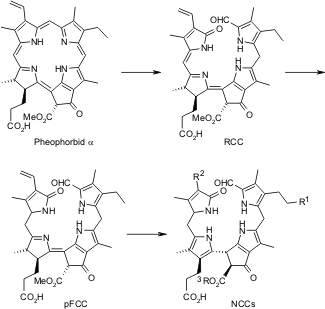
\includegraphics[scale=0.5]{figures/Kapitel2/VWA_Schema_Chlorophyllabbau.png}
  \caption[Abbauprozess des Chlorophylls, Quelle: http://www.organische-chemie.ch/chemie/2007nov/antioxidantien.shtm (Zugegriffen am: 05.11.2017)]{Abbauprozess des Chlorophylls in seneszenten Blättern}
  \label{fig:Chlorophyllabbau}
\end{figure}

Die Struktur eines \gls{Chl-K}en konnte erstmalig im Jahre 1991 aufgeklärt werden. Es handelte sich hierbei um einen \textit{Hv}-NCC der Gerste (\textit{Hordeum vulgare}) \cite{ErsterKatabolit}, das Endprodukt eines mehrstufigen Abbauprozesses. 

In den darauffolgenden Jahren fand man heraus, dass das Chlorophyll zuerst in das Pheophorbid a umgewandelt wird. Im nächsten Schritt wird der Makrozyklus oxygenolytisch (an der Reaktion beteiligtes Enzym: Pheo \textit{a} Mono-oxygenase \cite{ChlorophyllCatabolitesEnzyme}) in der nördlichen \textit{meso} Position geöffnet, woraufhin ein \textit{Red Chlorophyll Catabolite} (RCC) entsteht. 
Über einen \textit{primary flourescent Chlorophyll Catabolite} (pFCC) entsteht durch eine nichtenzymatische Isomerisierung ein \gls{NCC}. Thermodynamische Triebkraft dieser Reaktion ist die Rearomatisierung von Ring D. \cite{FCCKatabolit}, \cite{ChlorophyllCatabolites} Die unterschiedlichen Arten von \gls{NCC}s ergeben sich durch Anlagerung der entsprechenden funktionellen Gruppen (z. B. Zuckerring, Hydroxygruppe) an den pFCC. \cite{ChlorophyllCatabolites} 

\section{Nummerierung von Phyllobilinen}

\begin{figure}[!hbtp]
  \centering
  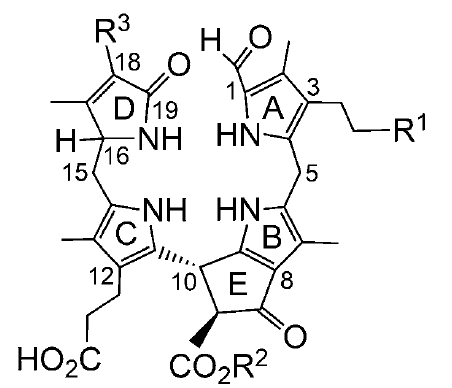
\includegraphics[scale=0.61]{figures/Kapitel2/VWA_Chl-Nummerierung.png}
  \caption[Nummerierung von Phyllobilinen, Quelle: Mathias Scherl]{Positionsangaben und Bezeichnungen der Ringe, die in der restlichen Arbeit für Ausführungen verwendet werden.}
  \label{fig:NummerierungPhyllobiline}
\end{figure}




\chapter{Methoden}

\section{HPLC}

Die \gls{hplc} ist eine chromatograpische Methode, um lösliche Stoffe analytisch und präparativ zu trennen. \cite[S. 165]{Chromatographie} 

Das Trennen der Stoffe basiert auf ihren unterschiedlichen chemischen Eigenschaften. Die Stoffe werden gelöst und bilden zusammen mit dem Laufmittel die mobile Phase, die an einer stationären Phase (in der Trennsäule) vorbeiströmt, wobei es zu Wechselwirkungen zwischen den gelösten Stoffen mit der stationären Phase kommt. Aufgrund der unterschiedlichen Affinität zu einer Phase hält sich jeder Stoff unterschiedlich lang in der stationären Phase auf. Die Verweildauer eines Stoffes in der Trennsäule wird als Retentionszeit bezeichnet. \cite[S. 31-32]{Chromatographie} Die Retentionszeit wird über Detektoren bestimmt, die die Änderung der Zusammensetzung der mobilen Phase feststellen und das Ergebnis in einem Chromatogramm darstellen. \cite[S. 46]{Chromatographie} 

Für die Experimente wurde die Methode der \gls{rp} Chromatographie angewandt. Dabei ist die mobile Phase polar und die stationäre Phase unpolar (als unpolare Phase dienen beispielsweise Silane mit langen Kohlenwasserstoffketten). \cite[S. 189]{Chromatographie}\\

Im Rahmen meiner Arbeit wurde die \gls{hplc} verwendet, um die Stoffe im seneszenten Blatt zu trennen und entsprechende \gls{Chl-K}en zu isolieren. Die Identifikation der \gls{Chl-K}en erfolgte dabei durch einen UV/Vis Detektor (200 nm - 800 nm) sowie durch ein dazu geschaltetes Massenspektrometer (=\gls{lcms}). Um die \gls{Chl-K}en mit einem hochauflösenden Massenspektrometer zu fragmentieren, wurden die Verbindungen zu jenen Zeiten, zu denen sie in der \gls{hplc} jeweils eluieren in \gls{eppi} gesammelt.\\

Die Herstellung eines Blattextraktes für die Analyse mit der \gls{hplc} wird in Kapitel \ref{sec:HPLCAufarbeitungderProbe} beschrieben. Aufgrund dieser speziellen Aufarbeitung des Blattes zählt die Methode der \gls{hplc} nicht mehr zur direkten Analyse. Sie wurde lediglich verwendet, um die Ergebnisse von MS Leafspray zu verifizieren.

\section{Massenspektrometrie}

Mithilfe eines Massenspektrometers kann die Masse eines Moleküls bestimmt werden. Aufgrund der Einfachheit der Methode und der sehr geringen benötigten Probenmenge ist das Massenspektrometer für eine Vielzahl an Anwendungen geeignet (\gls{zB} in der Forensik, Lebensmittelprüfung, Medikamentenprüfung, Analyse von Meteoriten). \cite[S. 1]{MassSpectrometry} Der jetzige Entwicklungsstand in der Massenspektrometrie ist vor allem den Entwicklungen der letzten vier Jahrzehnte zu verdanken. \cite[S. 6-9]{MassSpectrometry} \\

Um die Molekülmasse der Stoffe zu bestimmen, werden sie zuerst in Gasphasen-Ionen überführt. \cite[S. 15]{MassSpectrometry} Dabei gibt es unterschiedliche Methoden, diesen Zustand herbeizuführen, wie \gls{zB} Electron Ionization, Chemical Ionization und Field Ionization. \cite[S. 15-30]{MassSpectrometry} Nach der Ionisation werden sie im Massenanalysator nach ihrem \gls{mz} Verhältnis getrennt und im Detektor der Ionenstrom gemessen. Das Ergebnis wird in einem Massenspektrum festgehalten, in dem auf der Ordinate die relative Intensität der einzelnen Peaks und auf der Absizze das Verhältnis \gls{mz} aufgetragen werden. \\

In den Experimenten dieser Arbeit wurde zur Ionisation die \gls{ESI} Methode verwendet, die erstmalig das Messen von Proteinen mithilfe eines Massenspektrometers erlaubte und aufgrund ihrer hohen Empfindlichkeit gegenüber kleinen, polaren Molekülen mit einer \gls{hplc} kombiniert werden kann. Bei der \gls{ESI} Methode wird durch Anlegen einer Spannung von 3-6kV zwischen der Kapillare, aus der die Flüssigkeit kommt und der Gegenelektrode ein elektrisches Feld mit einer Stärke in der Größenordnung von $10^{6}$ $Vm^{-1}$ angelegt. Die erhaltenen geladenen Tröpfchen passieren ein Inertgas (in den meisten Fällen \gls{n2}) \gls{bzw} eine erhitzte Kapillare, um das \gls{lm} zu entfernen. Anschließend an diese Ionisation wird die Molekülmasse der Ionen bestimmt. \cite[S. 43-44]{MassSpectrometry} \\

Um die Chlorophyllkataboliten im Massenspektrometer zu analysieren, wurde sowohl die Methode der \gls{lcms} als auch die Methode des MS-Leafspray verwendet. 

\subsection{LC-MS}

Bei der Methode der LC-MS wird eine \gls{hplc} vor ein Massenspektrometer geschaltet. Dabei trennt die \gls{hplc} die Stoffe zuvor auf und eluiert sie anschließend in das Massenspektrometer. \cite[S. 217-218]{MassSpectrometry} Um die Flussrate bei atmosphärischem Druck zu verringern, wird nur ein Teil des direkt aus der \gls{hplc} kommenden Flusses zum Massenspektrometer hin abgezweigt. Ansonsten wäre die Flussrate zu hoch, was eine Ionisierung der Probe mithilfe einer \gls{ESI} - Quelle unmöglich machen würde. \cite[S. 221]{MassSpectrometry} 

Das Resultat ist je ein Chromatogramm der HPLC und des Massenspektrometers. Es wird somit zu jedem Zeitpunkt eines \gls{hplc}-Laufes ein UV/VIS Spektrum sowie ein Massenspektrum erzeugt. Aus dem UV/VIS Spektrum lässt sich schließen, ob es sich bei einem \gls{Chl-K}en um einen \gls{NCC}, \gls{DNCC} oder einen \gls{YCC} handelt. Aus dem Massenspektrum kann die Molekülmasse (in Da) mit allgegenwärtigen Fragmentierungen abgelesen werden. Unter Verwendung eines hochauflösenden Massenspektrometers wird außerdem die atomare Zusammensetzung in Form einer Summenformel ersichtlich. \\

\subsection{MS Leafspray} \label{sec:MSLeafspray}

\textit{Ambient Ionization} \cite{AmbientIonisation} ermöglicht es, Proben ohne vorherige präparative Trennung durch chromatographische Trennverfahren direkt in ihrer \textit{natürlichen} Umgebung mithilfe eines Massenspektrometers zu untersuchen. Eine Methode, die auf dem Prinzip der \textit{Ambient Ionization} basiert ist \textit{Paper Spray} \cite{PaperSpray}. Dabei  kommt es zu einer Kombination der \gls{ESI} sowie der \textit{Ambient} Ionisationsmethode. \cite{PaperSpray}\\

Die Ionisation der Probe erfolgt ausgehend von einem feuchten, porösen Material (\gls{zB} Papier), das in einer Kupferklemme eingeklemmt wird. Zwischen der Kapillaröffnung des Massenspektrometers und der Kupferklemme liegt eine Spannung im Bereich von 3-6kV an, woraufhin kleine Tröpfchen, die Ionen der Probe enthalten von der Spitze des porösen Materials ausgesendet werden und Ionen der Probe in das Massenspektrometer befördern. \cite{RapidScreeningLeafSpray} Durch Anlegen von Kalibrationskurven mit externen Standards wird außerdem ermöglicht, eine quantitative Bestimmung der Menge des Analyten durchzuführen. \cite{LeafSpray}

Leaf Spray ist eine Form von Paper Spray, bei der die zu analysierende Pflanze selbst als poröses Material dient. Sie wurde im Rahmen dieser Arbeit für die Identifikation von \gls{Chl-K}en verwendet. Ein Vorteil einer Analyse von \gls{Chl-K}en mit MS Leafspray ist, dass weniger Zeit für die Vorbereitung benötigt wird, was wiederum Grundlage für eine schnellere und effizientere Analyse ist. Genauere Ausführungen zur Durchführung finden sich in Kapitel \ref{sec:MSLeafspray}.\\



\addpart{Experimenteller Teil}

\chapter{Allgemeine Arbeits- und Analysemethoden}

\section{Herstellung von Lösungen für eine Analyse mit HPLC}

\begin{itemize}
\item Herstellung eines 3.2 mM \ch{NH4Ac} Puffers:

Es wurden 0.1542 g Ammoniumacetat abgewogen und in 0.5 L Wasser gelöst.

\end{itemize}

\section{Chemikalien und Material}

\section{Probenmaterial}

Als Probe dienten Brokkoliblätter der Brokkolipflanze aus dem Garten meiner Oma (Grundfeld Telfs, Austria). Die Brokkoliblätter wurden jeweils in der früh zwischen 07:20 und 07:30 gesammelt. Der Zeitraum, in dem die Brokkoliblätter für Analysen verwendet wurden beträgt maximal drei Tage (danach wurden neue Brokkoliblätter gesammelt). Der Untersuchungszeitraum erstreckt sich von 03.08.2017 bis zum 13.09.2017 (die letzten Brokkoliblätter wurden am 11.09.2017 gesammelt).\\

\section{Reaktion mit Essigsäureanhydrid}

Im Rahmen der direkten Analyse der \gls{Chl-K} wurden diese einer Reaktion mit Essigsäureanhydrid unterzogen. Die Reaktion wurde dabei direkt am Blatt durchgeführt. Dazu wurden in einem Exikator getrocknete Blätter auf eine Fläche von \gls{ca} 2cm\textsuperscript{2} (entspricht einer ungefähren Blattmasse von 0.01g) zugeschnitten und anschließend mit 300\si{\uL} Essigsäureanhydrid beidseitig benetzt. Die 300\si{\uL} ergaben sich, da das Blatt nicht in der Reagenz schwimmen sollte, da sonst Teile des Blattes aus diesem herausgelöst werden, was zu einer Verringerung der Intensitäten in \gls{hplc} und MS-Leafspray führt. 

Die Reaktion wurde durch eine Vakuumpumpe mit zwischengeschalteter Kühlfalle gestoppt (Verweildauer in der Vakuumpumpe betrug \gls{ca} 5min). Dabei wurde die Reagenz abgesaugt. 

Die Reaktionsdauer betrug zwischen 7min. und 6h. Für die Präsentation und Diskussion der MS-Leafspray Versuche wurden die Reaktionsprodukte nach 22min. Reaktionsdauer verwendet, wohingegen für die Präsentation der \gls{hplc} Versuche die Reaktionsprodukte nach 3h Reaktionsdauer.

\section{Erstellen von Fragmentierungsdiagrammen} \label{sec:fragmentierungsdiagramme}

Zu jedem \gls{Chl-K} wurde ein Fragmentierungsdiagramm erstellt. Dazu werden die Intensitäten der einzelnen beobachteten Fragmentierungen im Massenspektrometer zur jeweiligen aufgewendeten, \gls{nKE} (alle fünf Einheitsschritte) aufgenommen. 

Auf der Abszisse des erhaltenen Diagramms befindet sich die \gls{nKE} und auf der Ordinate die Intensität der jeweiligen Fragmentierung bezogen auf den höchsten Peak, der während der Aufnahme beobachtet wurde (ebenfalls in Prozent). 

Die erhaltenen Kurven wurden mit einem Savitzky-Golay Filter geglättet (siehe Anhang) und werden im folgenden als Fragmentierungsdiagramme bezeichnet. Ein Nachteil bei der Behandlung mit diesem Filter ist, dass in manchen Fällen die Intensitäten der Fragmentierungen bei einer normalisierten Kollisionsenergie von null nicht gleich null sind. Es wird im folgenden angenommen, dass dies dennoch so ist.

Aufgenommen wurden die Fragmentierungsdiagramme im \gls{cid} und im \gls{pqd} Modus.\\

Es wird damit versucht, herauszufinden, ob bestimmte Abspaltungen der Kataboliten charakteristische Muster aufweisen, um in weiterer Hinsicht weitere strukturelle Eigenschaften über die Kataboliten mithilfe eines Massenspektrometers zu erfahren. Weiters wird ein Vergleich zwischen den Fragmentierungsdiagrammen von MS Leafspray und des hochauflösenden Massenspektrometers versucht. Für diesen Vergleich wurden nur die Diagramme verwendet, die im \gls{cid} Modus aufgenommen wurden, da das verwendete Massenspektrometer von MS-Leafspray nur in diesem Modus operieren konnte.
\chapter{Experimente MS Leafspray}

\section{Massenspektrometer}

(Beschreibung Massenspektrometer)

\section{Versuchsaufbau} \label{sec:Versuchsaufbau}

Abbildung \ref{fig:LeafsprayVersuchsaufbau} beschreibt schematisch den Versuchsaufbau. 

\begin{figure}[!hbtp]
  \centering
  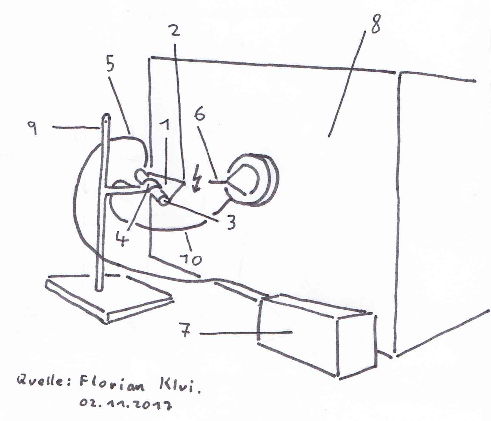
\includegraphics[scale=0.5]{figures/Kapitel4/VWA_MSLeafspray_Versuchsaufbau.png}
  \caption[Leafspray Versuchsaufbau, Quelle: Author]{Leafspray Versuchsaufbau: 1) Filterpapierdreick, 2) Spitze des Dreiecks, 3) Blattmaterial, von Filterpapier umschlossen, 4) Kupferklemme, 5) Kapillare für \gls{lm}, 6) Einlass des Massenspektrometers (mit der markanten Spitze zwecks Verdeutlichung etwas übertrieben dargestellt), 7) \textit{Syringe Pump}-kontrolliert den \gls{lm}-Fluss durch 5), 8) Massenspektrometer, 9) Stativ, 10) Kabel, mit 4) verbunden-zwischen 4) und 6) liegt eine Spannung (3-6kV) an (durch Blitz zwischen 2) und 6) symbolisiert)}
  \label{fig:LeafsprayVersuchsaufbau}
\end{figure}

Das zu analysierende Blatt wurde in Filterpapier eingerollt und das Filterpapierdreieck wurde in einer Kupferklemme eingespannt (Kapitel \ref{sec:Versuchsdurchfuehrung}). Die Kupferklemme wurde mit einem Kabel (10), das mit dem Massenspektrometer (8) verbunden war, verbunden. Zwischen der Kupferklemme (4) und dem Massenspektrometer wurde eine Spannung zwischen 3-6kV angelegt. Da das Filterpapier mit \gls{lm} benetzt ist und eine Verbindung zur Kupferklemme besteht, kommt es zu einer durch die Spannung ausgelösten Bewegung der im \gls{lm} gelösten Ionen, die in das Massenspektrometer hineinfliegen. Der Abstand zwischen Filterpapier (2) und Einlass des Massenspektrometers (6) betrug ungefähr 0.5cm und ist damit der Flugstrecke der Ionen gleichzusetzen. 

\begin{figure}[htbp]
  \begin{subfigure}[b]{0.5\textwidth}
    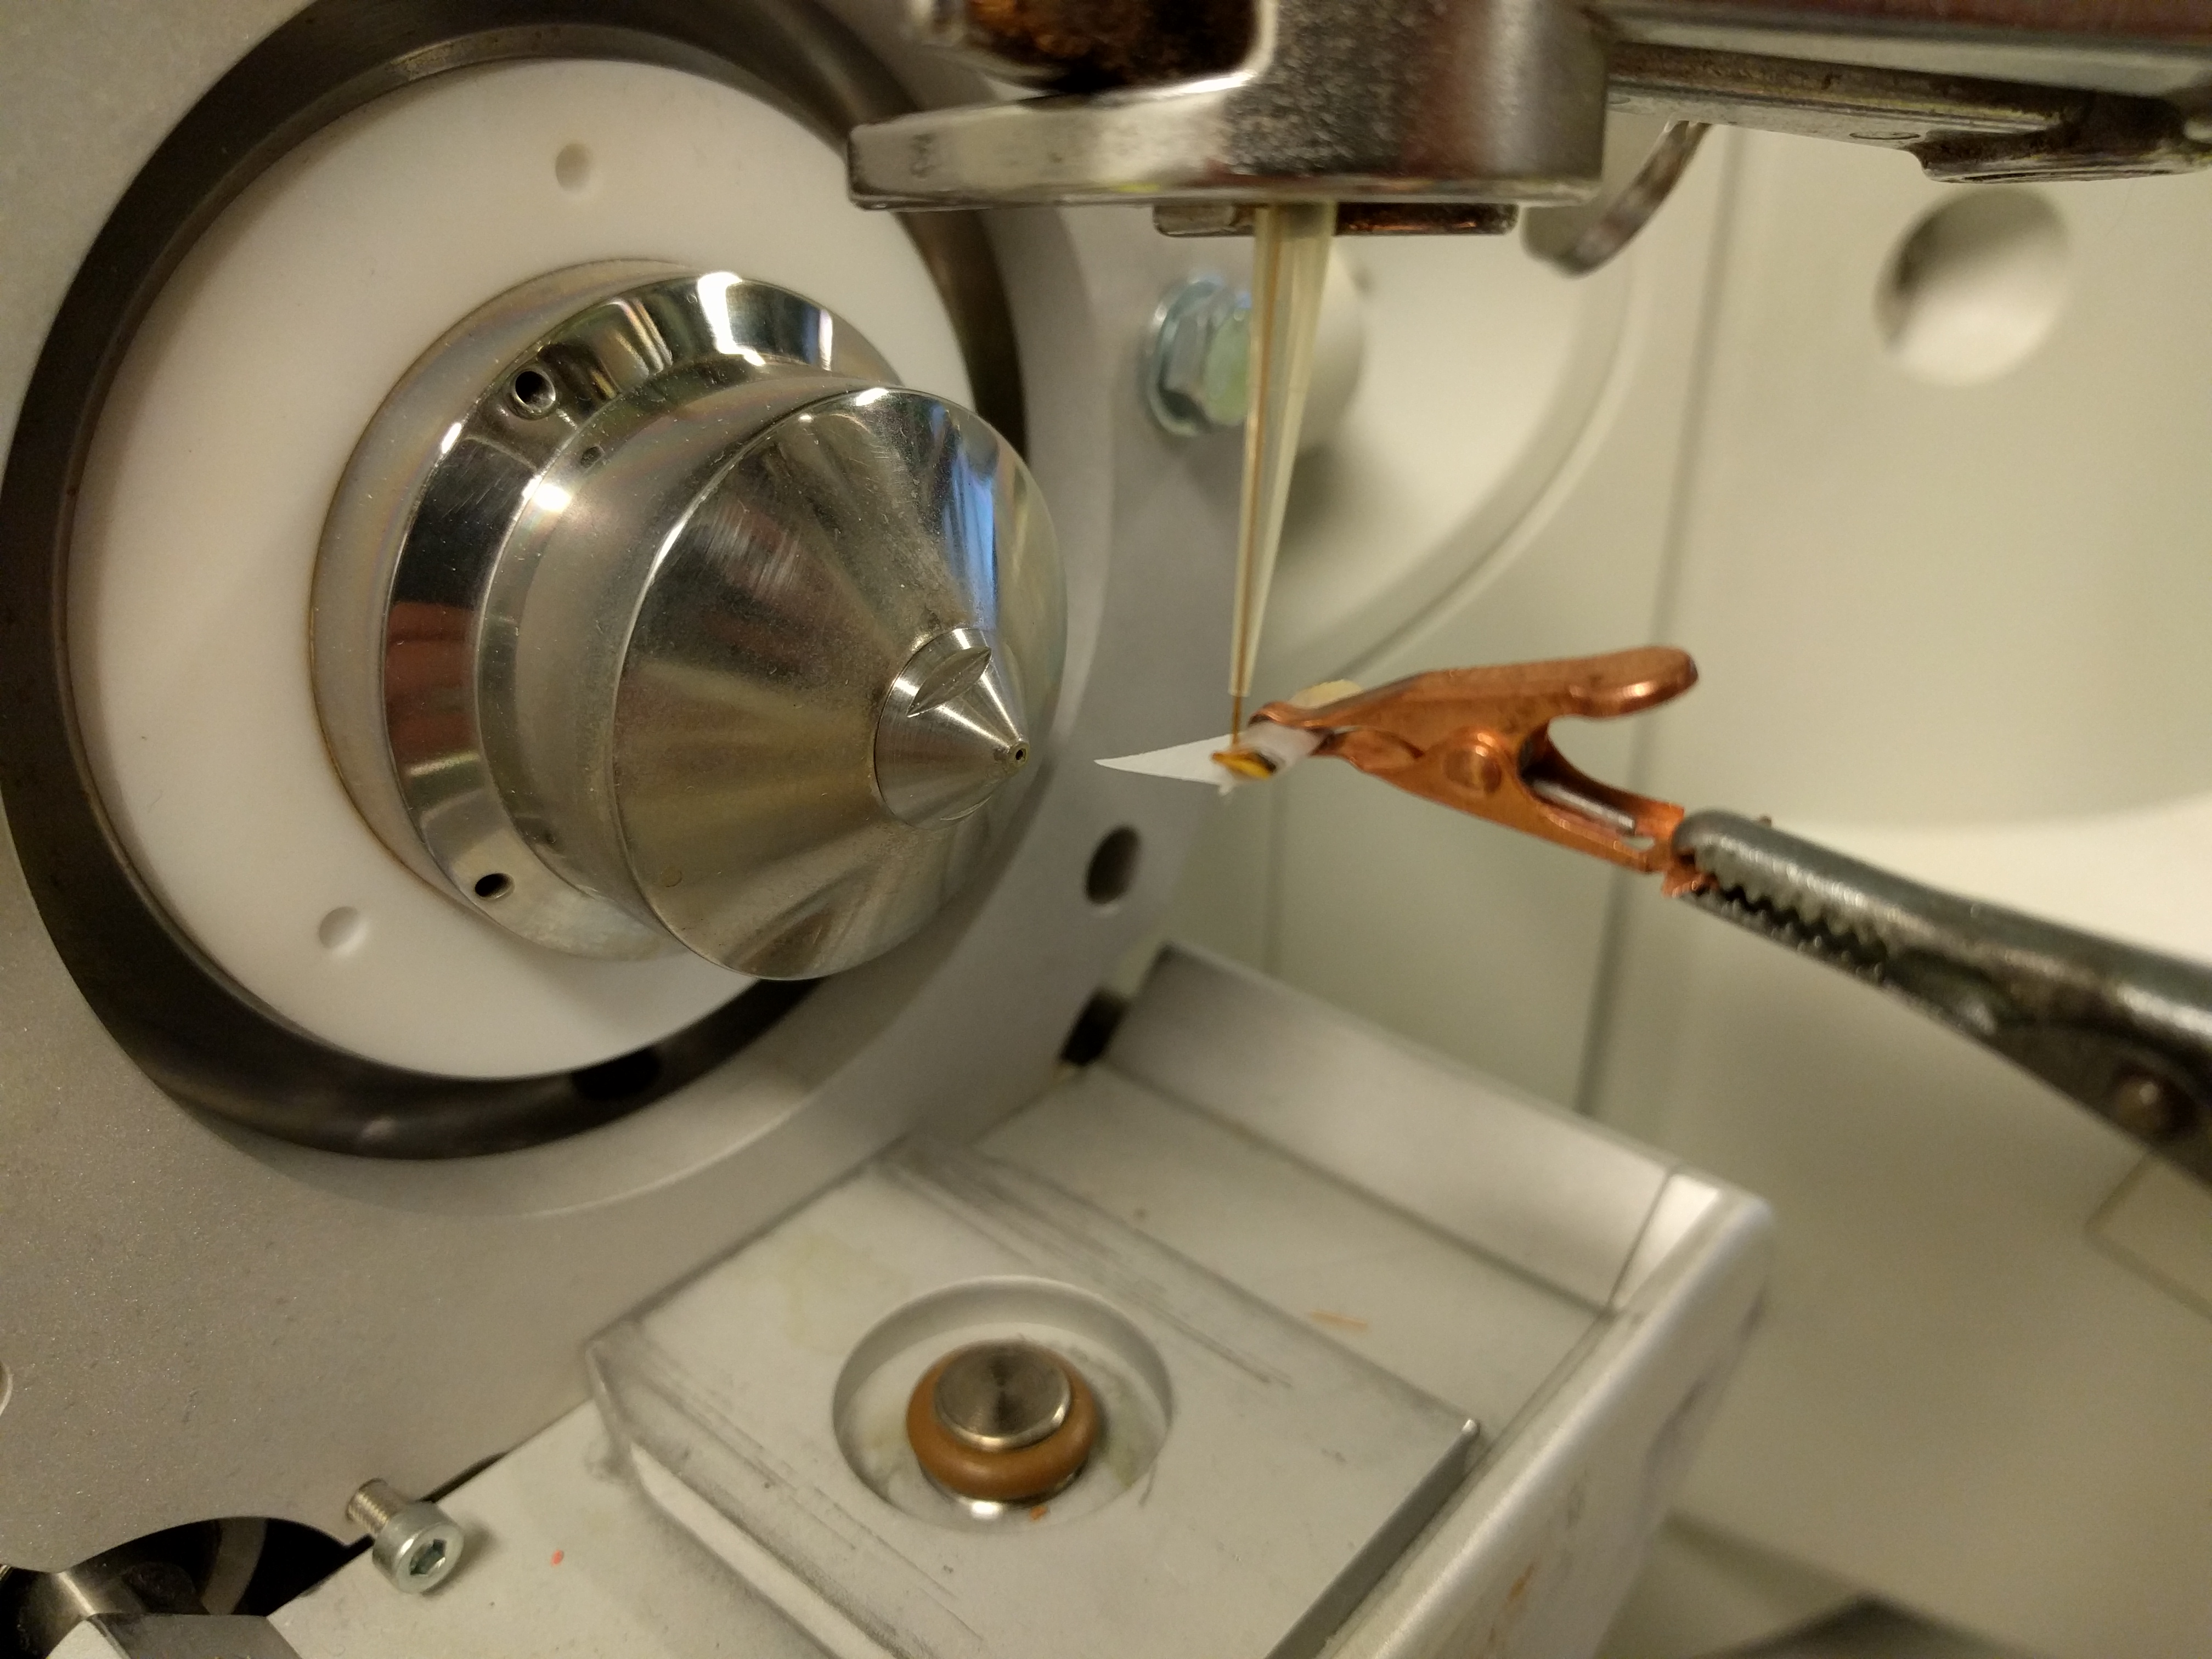
\includegraphics[width=\textwidth]{figures/Kapitel4/VWA_MSLeafspray_Detail1.jpg}
    \caption{}
    \label{fig:MSLeafsprayDetail1}
  \end{subfigure}
  \hfill
  \begin{subfigure}[b]{0.5\textwidth}
    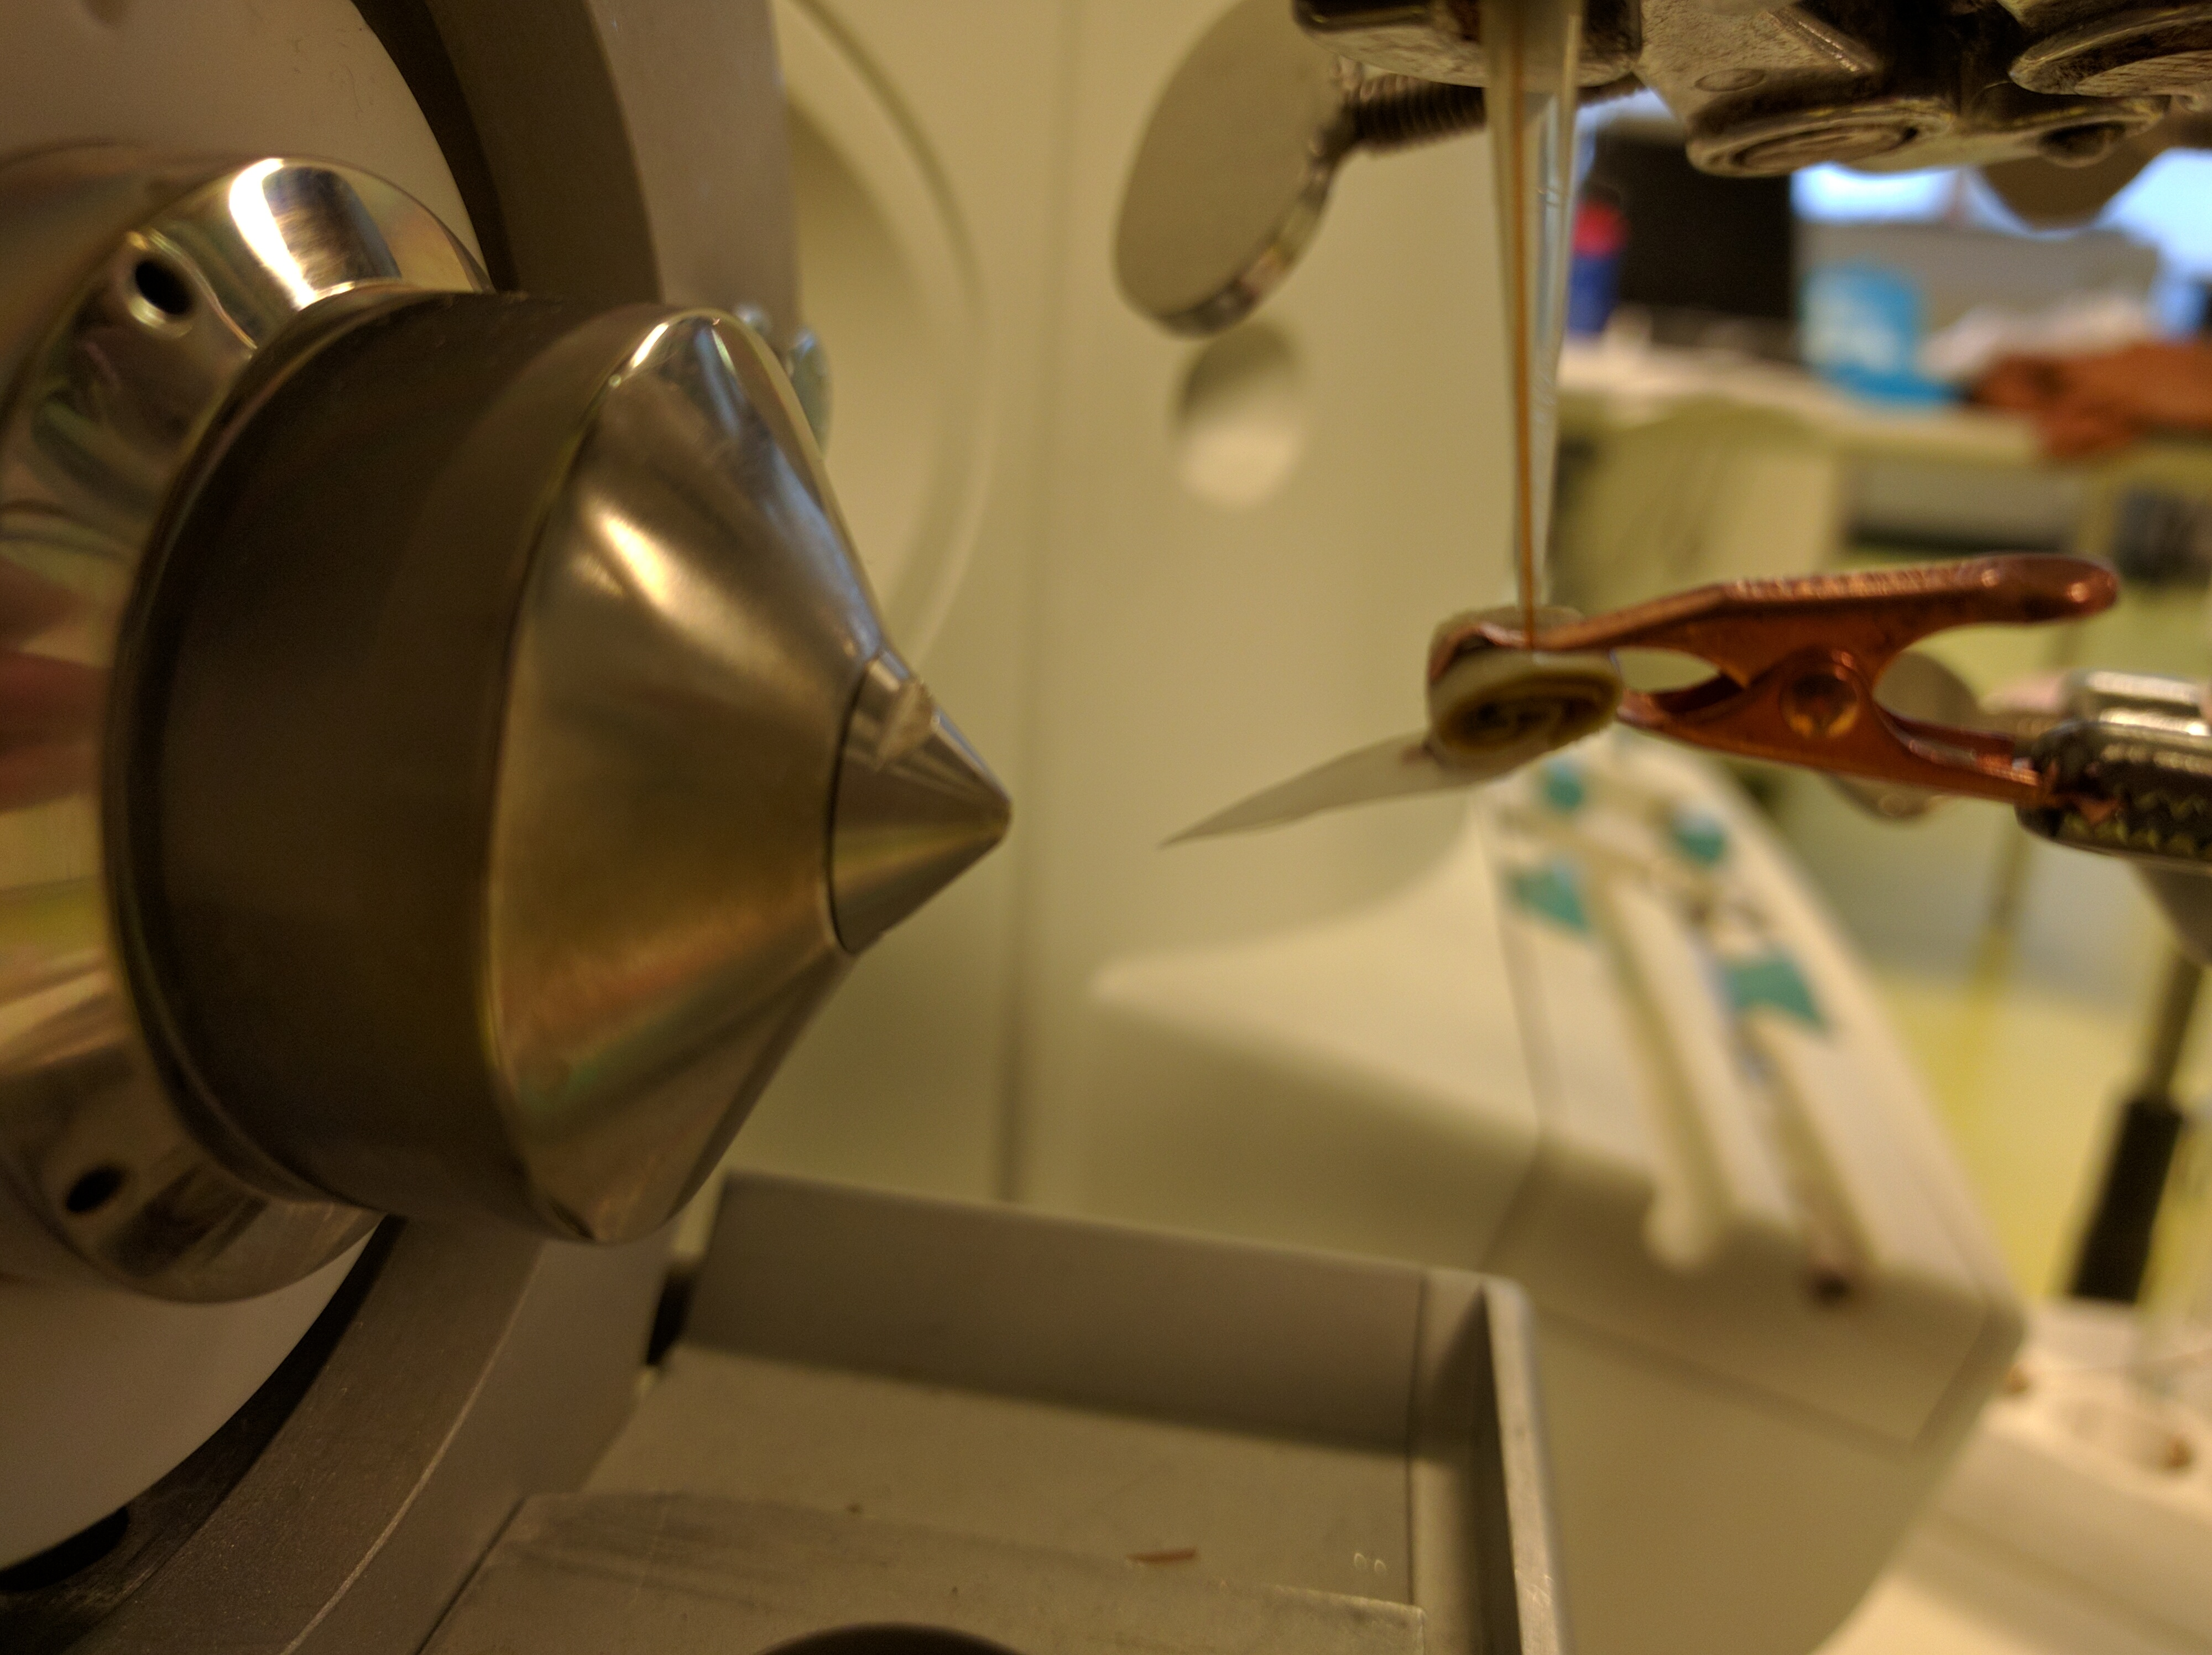
\includegraphics[width=\textwidth]{figures/Kapitel4/VWA_MSLeafspray_Detail2.jpg}
    \caption{}
    \label{fig:MSLeafsprayDetail2}
  \end{subfigure}
  \label{fig:MSLeafsprayDetail}
  \caption[MS Leafspray Versuchsaufbau Detailfotos, Quelle: Author]{(a) Einlass des Massenspektrometers mit Kapillare, Kupferklemme und Filterpapier mit Blattmaterial, (b) Detailansicht}
\end{figure}

In Abbildung \ref{fig:MSLeafsprayDetail1} wird gezeigt, wie diese Anordnung umgesetzt wurde. Zu sehen sind die Kupferklemme mit dem eingespannten Filterpapier und dem darin enthaltenen Blatt, die \gls{lm}-Kapillare, die Einlassöffnung des Massenspektrometers und der Abstand von Filterpapierdreicksspitze zum Massenspektrometer. Es gilt zu beachten, dass das Blatt in einem gewissen Winkel eingespannt wird, um zu verhindern, dass das \gls{lm} nicht abfließt, was bei einer waagrechten Anordnung auftreten kann. 

\section{Versuchsdurchführung} \label{sec:Versuchsdurchfuehrung}

Frisch gesammelte Brokkoliblätter und Filterpapier wurden mit Rasierklinge und Schere wie in Abbildung \ref{fig:LeafsprayVorbereitung}a ersichtlich zugeschnitten. Anschließend wurde das Brokkoliblatt auf das Filterpapier gelegt und dieses bis zur Basis des Dreiecks eingerollt. 

Diese Art der Vorbereitung zeigte sich als besonders effektiv, da mit ihr höhere Intensitäten der Signale im Massenspektrometer erreicht werden konnten, wie wenn nur das Blatt zu einem Dreieck zugeschnitten und in dieser Form vor das Massenspektrometer gehalten wird. Grund dafür ist vermutlich, dass das \gls{lm} mehr Zeit hat, die Chlorophyllkataboliten aus dem Blatt heraus zu lösen und dass mehr Blattmaterial vorhanden ist. Außerdem behält das Filterpapier länger seine Steifigkeit wie ein Brokkoliblatt, weswegen längere Analysen mit konstanterem Signal möglich sind.

\begin{figure}[hbtp]
  \centering
  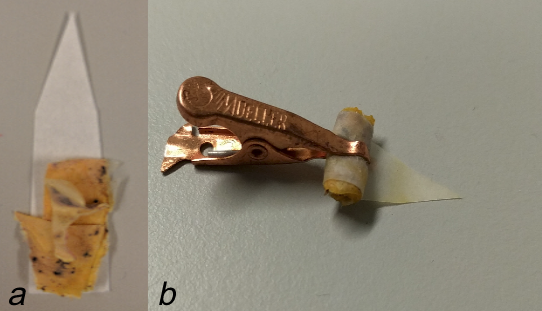
\includegraphics[scale=0.5]{figures/Kapitel4/VWA_MSLeafspray_Blattvobereitung_zwei.png}
  \caption[Leafspray Blattvorbereitung, Quelle: Author]{Leafspray Blattvorbereitung: a) zugeschnittenes Filterpapierdreieck, mit frischen, seneszenten Brokkoliblättern, b) eingerolltes \textit{Päckchen}, in Kuperklemme eingespannt}
  \label{fig:LeafsprayVorbereitung}
\end{figure}

Das erhaltene \textit{Päckchen} wurde durch eine Kupferklemme ca. 0.5cm (Abbildung \ref{fig:LeafsprayVorbereitung}b) vor die Kapillare des Massenspektrometers gehalten. Um ein konstantes Signal zu erhalten versorgte eine Kapillare, die wie in Abbildung befestigt war, das Päckchen mit einem konstanten \gls{lm}-Fluss (als \gls{lm} dienten \gls{meoh} sowie Acetonitril). Die Flussrate des \gls{lm} betrug zu Beginn 12\si{\uL\per\minute}, um das Blatt schneller zu befeuchten und wurde ab dem Erhalt des ersten Signals auf 5\si{\uL\per\minute} zurückgefahren. Es zeigte sich, dass bei dieser Flussrate das Signal bei gleichbleibend hoher Intensität am längsten bleibt. Der Spraystrom betrug zwischen xx und xx \si{\micro\ampere}. Diese Einstellungen und Aufarbeitungsmethoden ermöglichten das Messen der Fragmentierungsdiagramme, da hierfür eine längere Analysezeit vonnöten ist.\\

\textit{(Platz für Beschreibung der Einstellungen des Gerätes)}\\

Aufgenommen wurden die Massenspektrum im Bereich von 300 \gls{mz} bis 1000 \gls{mz}, um  Massenspektren zu bekommen, die nicht so stark von anderen Ionensorten gestört werden. Gemessen wurde im positiven Ionenmodus, wobei zwischendurch in den negativen Ionenmodus gewechselt wurde, wenn die Intensität des Signals im positiven Ionenmodus abnahm. Das Wechseln des Modus konnte die gewünschte Intensität wieder erhöhen. Es konnte somit ein ähnliches Verhalten der Intensitäten im Zeitverlauf beobachtet werden wie in \cite{RapidScreeningLeafSpray} bereits beschrieben, wobei hier das Umschalten in den negativen Ionenmodus nicht explizit erwähnt wird, um das Problem der abnehmenden Intensitäten im positiven Ionenmodus zu beheben.

\section{Chlorophyllkataboliten des Brokkoliblattes}

Im Folgenden werden die Chlorophyllkataboliten beschrieben, die sich durch MS Leafspray identifizieren ließen. Die Strukturvorschläge wurden durch hochauflösende Massenspektrometrie überprüft. Sie beruhen auf den exakten Molekülmassen und den daraus errechneten möglichen Summenformeln.

Fragmentierungsdiagramme wurden wie in \ref{sec:fragmentierungsdiagramme} beschrieben, erstellt.

\subsection{Bo-NCC-1}

Beim Bo-NCC-1 handelt es sich um einen strukturidenten Kataboliten, wie er auch in der Brokkolifrucht gefunden wurde. \cite{ChlorophyllCatabolitesBroccoli} Gefunden wurde die protonierte Verbindung bei m/z = 793 [M+H]\textsuperscript{+} und das Kaliumsalz bei m/z = 831 [M+K]\textsuperscript{+}. Aufgrund der geringen Intensitäten der protonierten Verbindung war es nicht möglich, ein verwertbares Massenspektrum dieser aufzunehmen. 

Der Katabolit bei m/z = 831 [M+K]\textsuperscript{+} zeigt Abspaltungen von \ch{H2O} bei m/z = 813 [M - \ch{H2O} + K]\textsuperscript{+}, von \ch{CO2} bei m/z = 787 [M - \ch{CO2} + K]\textsuperscript{+} und eine Folge von Abspaltungen bei m/z = 311 [M - (Ring A, Ring D, Zucker, \ch{CO2}) + K]\textsuperscript{+}, bei der Ring A mit dem Zucker, Ring D sowie \ch{CO2} abgespalten wird (siehe Kapitel, Katabolit 619, hochauflösende Massenspektrometrie). Die Abspaltungen bei m/z = 798 [M - (\gls{nAb}) + K]\textsuperscript{+}, m/z = 586 [M - (\gls{nAb}) + K]\textsuperscript{+} und m/z = 551 [M - (\gls{nAb}) + K]\textsuperscript{+} können nicht eindeutig zugeordnet werden, da hierzu weitere experimentelle Daten vonnöten sind. Das Fragment bei m/z = 798 [M - (\gls{meoh}?) + K]\textsuperscript{+} ist insofern interessant, da es sich hierbei um eine Abspaltung von \gls{meoh} (-32 Da) handeln könnte (es wird angenommen, dass die Abweichung um eins durch Ungenauigkeiten des Massenspektrometers zustandekommt), was aber nicht mit der Struktur des Bo-NCC-1 (siehe Abbildung \ref{fig:831MKLeafspraystructure}) vereinbar ist. Aufgrunde ihrer Ungeklärtheit wird auf diese Abspaltung in den weiteren Ausführungen nicht näher eingegangen.

\begin{figure}[htbp]
  
  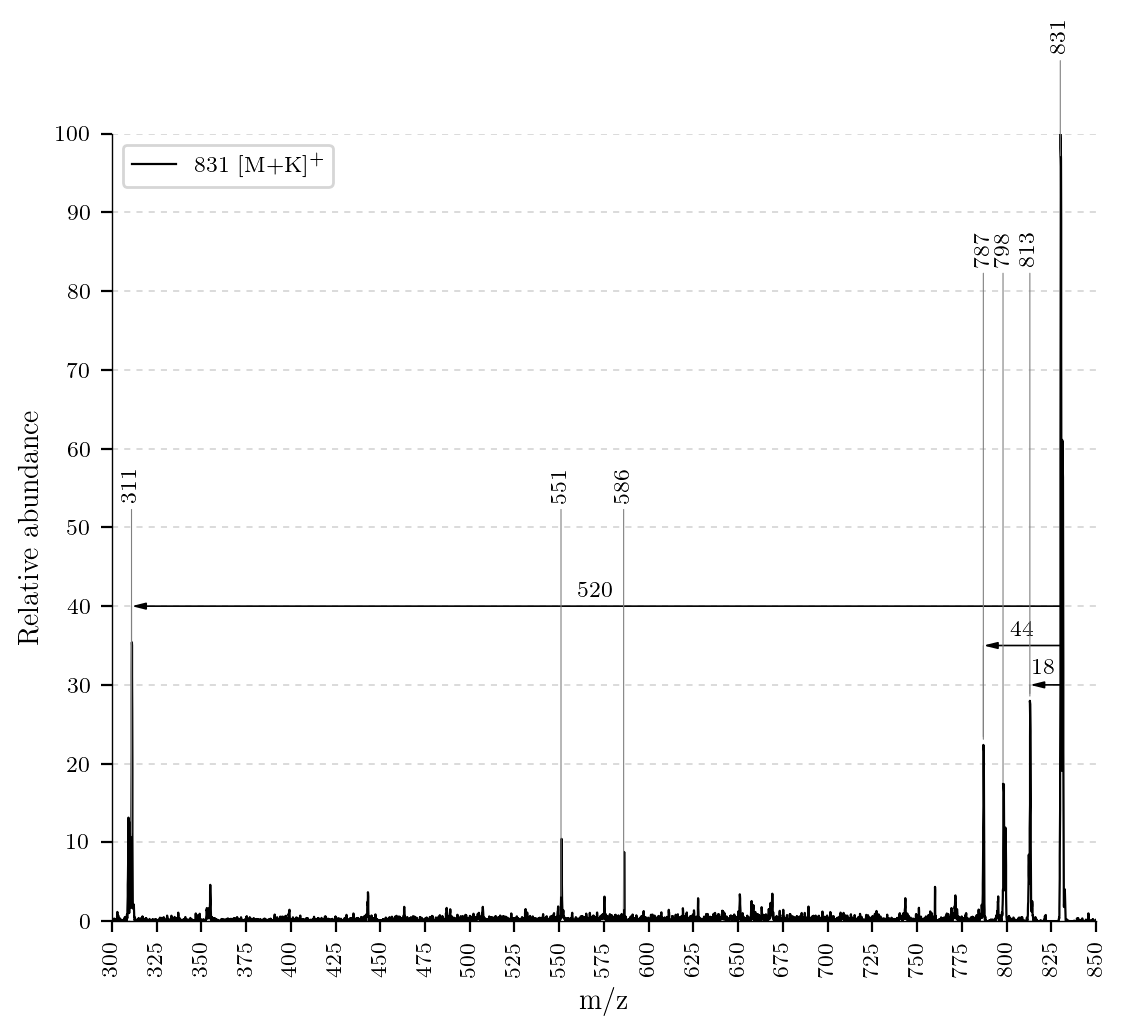
\includegraphics[width=\textwidth, height=0.7\textwidth]{figures/Kapitel4/Kataboliten/VWA_MS_LeafSpray_831.png}
  \label{fig:831MKLeafspray}
  
  \caption[ESI-MS Spektrum von Bo-NCC-1, Quelle: Author]{ESI-MS von Bo-NCC-1 mit m/z = 831 [M+K]\textsuperscript{+}}
\end{figure}

Wie aus dem Fragmentierungsdiagramm (Abbildung \ref{fig:831MKLeafspraydiags}) ersichtlich, erfolgt die Abspaltung von \ch{H2O} bei niedrigeren Energie wie jene von \ch{CO2} und verschwindet bei höheren Energien, wohingegen die Abspaltung von \ch{CO2} erhalten bleibt. Die Abspaltung von \ch{H2O} erreicht ein lokales Maximum bei einer \gls{nKE} von 10. Die Abspaltung erreicht ein lokales Maximum bei 30 \gls{nKE}.

Aufgrund der \ch{CO2} Abspaltung wird an Position .. eine Carbonsäuregrupper vermutet (wie in \cite{StructureElucidation} gezeigt), die über einen Mechanismus wie in Abbildung .. vorgeschlagen, abgespalten wird. Die relativ große Molekülmasse weist auf einen Zucker an Position .. hin. Die Summenformel des Bo-NCC-1 konnte über die exakte Molekülmasse mit einem hochauflösenden Massenspektrometer bestimmt werden.

\begin{figure}[htbp]
  \begin{subfigure}[b]{0.5\textwidth}
    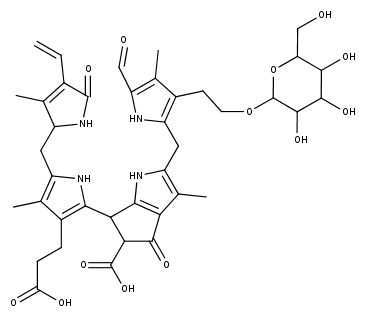
\includegraphics[width=\textwidth]{figures/Kapitel4/Kataboliten/fragmentation_structures/VWA_Katabolit_831.png}
    \caption{}
    \label{fig:831MKLeafspraystructure}
  \end{subfigure}
  \hfill
  \begin{subfigure}[b]{0.5\textwidth}
    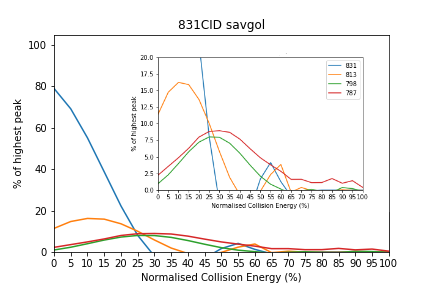
\includegraphics[width=\textwidth]{figures/Kapitel4/Kataboliten/diags/831CID-savgol.png}
    \caption{}
    \label{fig:831MKLeafspraydiags}
  \end{subfigure}
  \caption[Strukturvorschlag von Bo-NCC-1 und Fragmentierungsdiagramm, Quelle: Author]{(a) Strukturvorschlag des Bo-NCC-1 mit Summenformel \ch{C40H48N4O13}, (b) Fragmentierungsdiagramm von Bo-NCC-1 (blau = 831 [M+K]\textsuperscript{+}, orange = 813 [M - \ch{H2O} + K]\textsuperscript{+}, grün = 798 [M - (\ch{MeOH} - \gls{nAb}) + K]\textsuperscript{+}, rot = 787 [M - \ch{CO2} + K]\textsuperscript{+})}
\end{figure}



\subsection{Bo-NCC-3}

Beim Bo-NCC-3 handelt es sich um einen Kataboliten, der nicht in der Brokkolifrucht identifiziert wurde, weswegen er als dritter, in der Brokkolipflanze gefundener Katabolit den Index 3 erhält. \cite{ChlorophyllCatabolitesBroccoli} Analysiert wurde das Kaliumsalz mit m/z = 685 [M+K]\textsuperscript{+}. 

Es wurden zwei charakteristische Abspaltungen von \ch{H2O} bei m/z = 667 [M - \ch{H2O} + K]\textsuperscript{+} sowie von \ch{CO2} bei m/z = 641 [M - \ch{CO2} + K]\textsuperscript{+} beobachtet. Bei den Abspaltungen bei m/z = 429 [M - (\gls{nAb}) + K]\textsuperscript{+}, m/z = 561 [M - (\gls{nAb}) + K]\textsuperscript{+}, m/z = 605 [M - (\gls{nAb}) + K]\textsuperscript{+} und m/z = 652 [M - (\gls{nAb}) + K]\textsuperscript{+} ist nicht eindeutig geklärt, welche Fragmente hierbei entstanden sind. Für das Fragment bei m/z = 652 [M - (\gls{meoh}?) + K]\textsuperscript{+} gilt das gleiche wie bei der Abspaltung von m/z = 798 [M - (\ch{MeOH}?) + K]\textsuperscript{+} von Bo-NCC-1. Um diese Fragmente aufzuklären müssten weitere Experimente des Kaliumsalzes mit einem hochauflösenden Massenspektrometer durchgeführt werden. Fragmentierungen der protonierten Verbindung konnten mit einem hochauflösenden Massenspektrometer identifiziert werden.

\begin{figure}[htbp]
  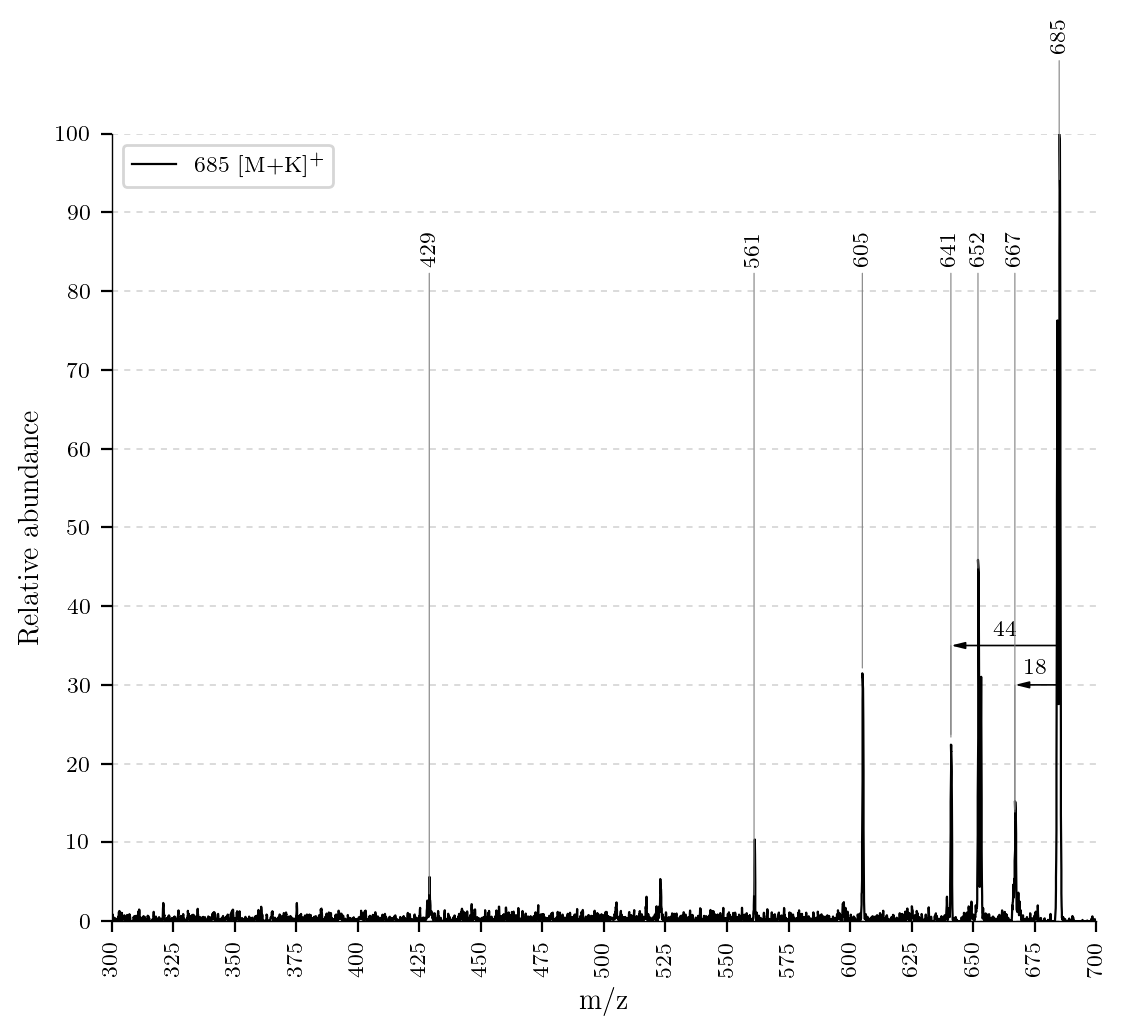
\includegraphics[width=\textwidth, height=0.5\textwidth]{figures/Kapitel4/Kataboliten/VWA_MS_LeafSpray_685.png}
  \label{fig:685MKLeafspray}
  
  \caption[ESI-MS von Bo-NCC-3, Quelle: Author]{ESI-MS von Bo-NCC-3 mit m/z = 685 [M+K]\textsuperscript{+}}
\end{figure}

\begin{figure}[htbp]
  \begin{subfigure}[b]{0.5\textwidth}
    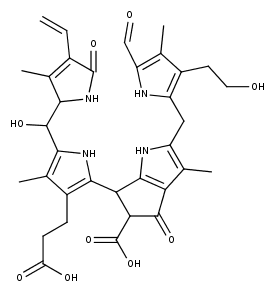
\includegraphics[width=\textwidth]{figures/Kapitel4/Kataboliten/fragmentation_structures/VWA_Katabolit_685.png}
    \caption{}
    \label{fig:685MKLeafspraystructure}
  \end{subfigure}
  \hfill
  \begin{subfigure}[b]{0.5\textwidth}
    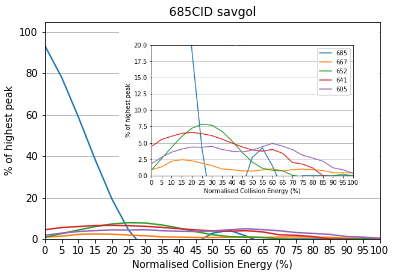
\includegraphics[width=\textwidth]{figures/Kapitel4/Kataboliten/diags/685CID-savgol.png}
    \caption{}
    \label{fig:685MKLeafspraydiags}
  \end{subfigure}
  \caption[Strukturvorschlag von Bo-NCC-3 und Fragmentierungsdiagramm, Quelle: Author]{(a) Strukturvorschlag von Bo-NCC-3 mit Summenformel \ch{C34H38N4O9}, (b) Fragmentierungsdiagramm von Bo-NCC-3 (blau = 685 [M+K]\textsuperscript{+}, orange = 667 [M - \ch{H2O} + K]\textsuperscript{+}, grün = 652 [M - (\gls{meoh}?) + K]\textsuperscript{+}, rot = 641 [M - \ch{CO2} + K]\textsuperscript{+}, violett = 605 [M - (\gls{nAb}) + K]\textsuperscript{+})}
\end{figure}

Das Fragmentierungsdiagramm zeigt, dass die Abspaltung von \ch{H2O} bei einer niedrigeren \gls{nKE} erfolgt, wie jene von \ch{CO2}, da sie ihre höchste Intensität zuvor erreicht (\gls{nKE} von 15 im Vergleich zu 20 von \ch{CO2}). Im Vergleich zum Bo-NCC-1 hat der Graph ein lokales Maximum der \ch{H2O} Abspaltung bei höheren Energien (beim Bo-NCC-3 bei 15 \gls{nKE} - beim Bo-NCC-1 bereits bei 10 \gls{nKE}). Das lokale Maximum der \ch{CO2} Abspaltung verschiebt sich von 30 \gls{nKE} beim Bo-NCC-1 auf 20 \gls{nKE} beim Bo-NCC-3 (Abbildungen \ref{fig:831MKLeafspraydiags} und \ref{fig:685MKLeafspraydiags}). Die potentiellen Abspaltungen von \gls{meoh} bei m/z = 652 [M - (\gls{nAb}) + K]\textsuperscript{+} und bei m/z = 605 [M - (\gls{nAb}) + K]\textsuperscript{+} werden nicht in diese Betrachtungen mit aufgenommen, da ihre Sinnhaftigkeit nicht geklärt ist.

Wie beim Bo-NCC-1 weist die \ch{CO2} Abspaltung auf eine freie Carbonsäure an Position .. hin. Aufgrund der durch die Summenformel erhaltene Sauerstoffanzahl wird angenommen, dass sich an Position .. eine Hydroxygruppe befindet (Abbildung \ref{fig:685MKLeafspraystructure}). Es wird vermutet, dass es sich dabei um eine Vorstuffe zu einem \gls{YCC} handelt. [Referenz]

\subsection{Bo-DNCC}

Es wird vermutet, dass der Bo-DNCC des Brokkoliblattes ident ist mit dem Bo-DNCC der Brokkolifrucht. \cite{ChlorophyllCatabolitesBroccoli} Beobachtet wurden zwei Pseudo-Molekulare Ionen. Eines mit m/z = 619 [M+H]\textsuperscript{+} (Abbildung \ref{fig:619MHLeafspray}) und mit m/z = 657 [M+K]\textsuperscript{+} (Abbildung \ref{fig:657MKLeafspray}).


\begin{figure}[htbp]
  \begin{subfigure}[b]{0.5\textwidth}
    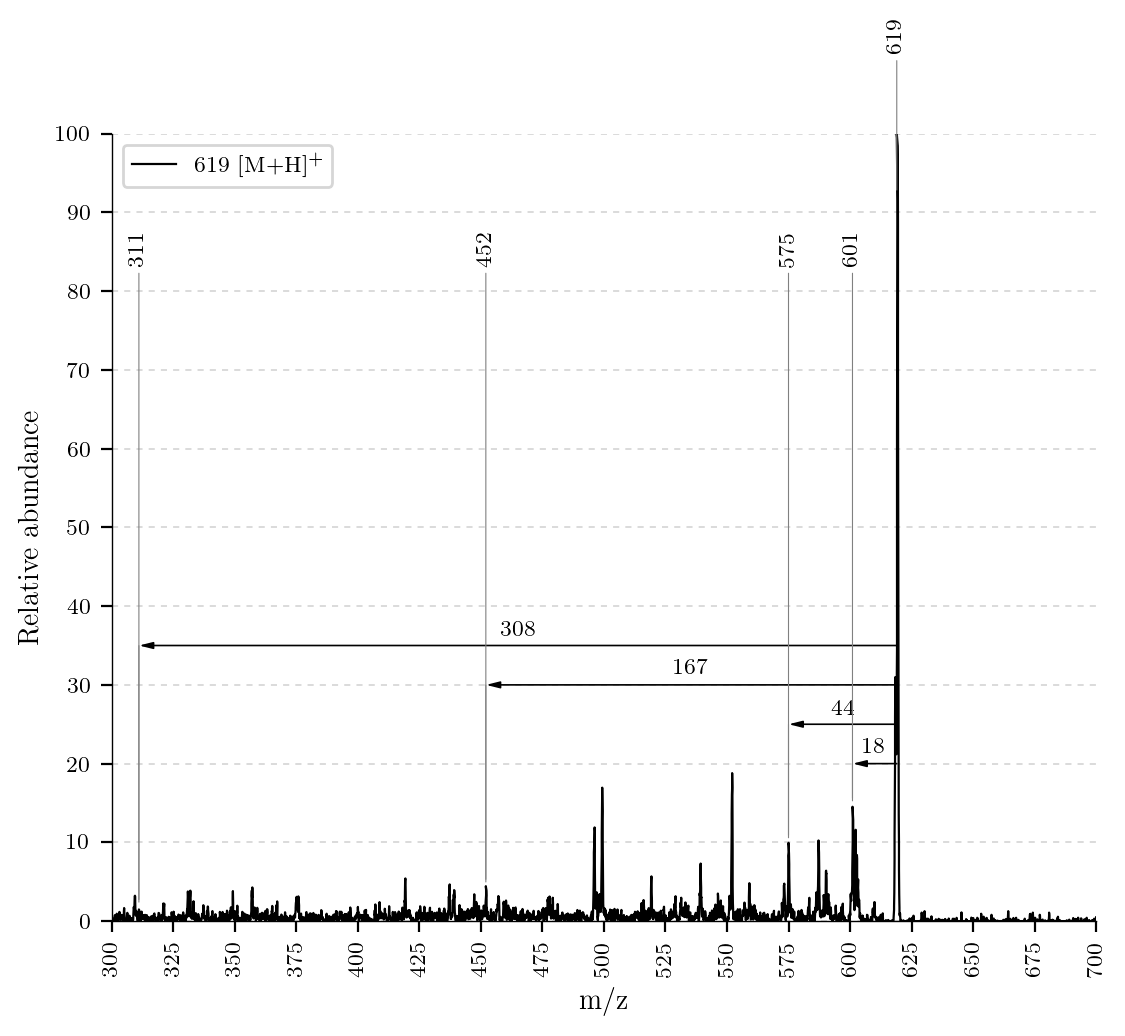
\includegraphics[width=\textwidth]{figures/Kapitel4/Kataboliten/VWA_MS_LeafSpray_619.png}
    \caption{}
    \label{fig:619MHLeafspray}
  \end{subfigure}
  \hfill
  \begin{subfigure}[b]{0.5\textwidth}
    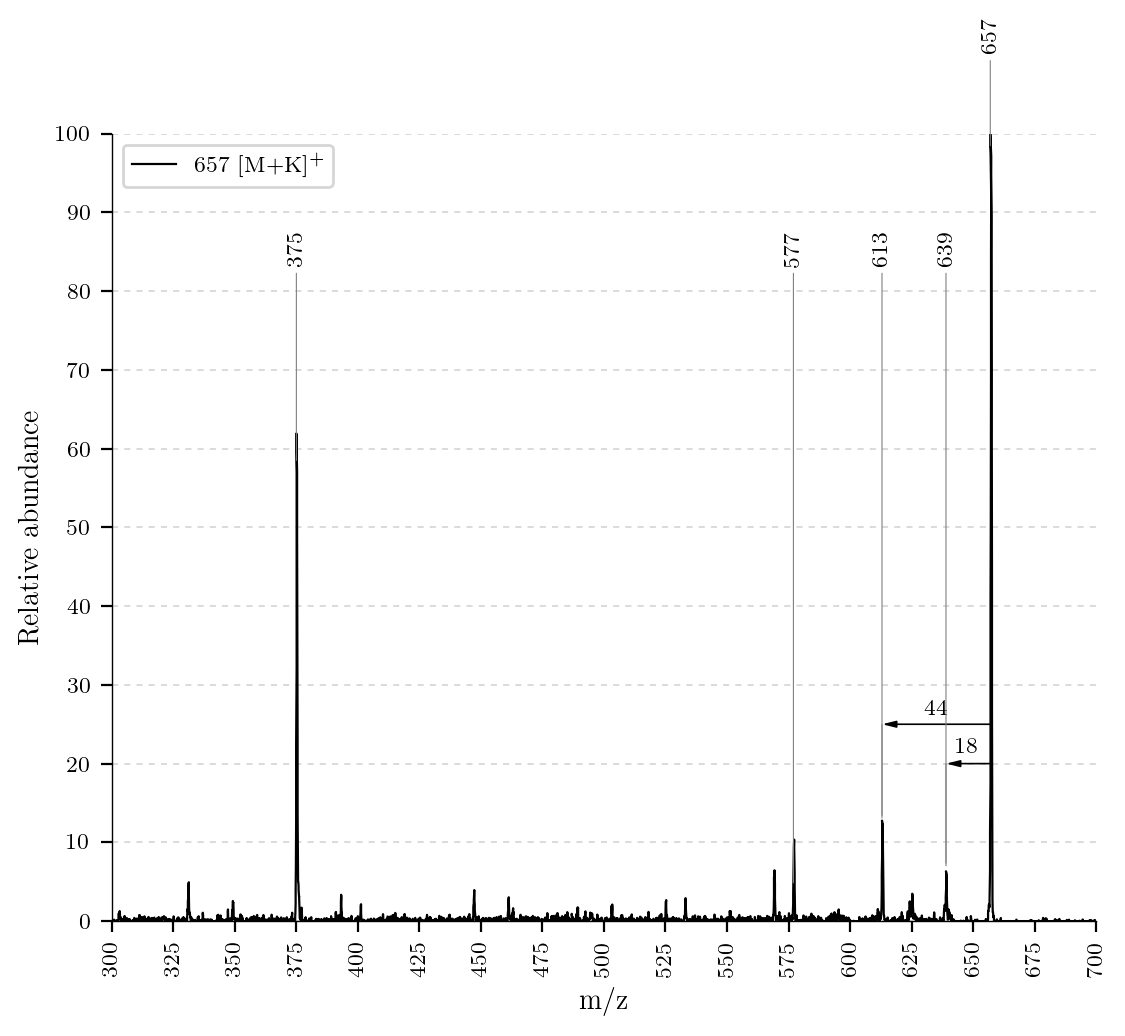
\includegraphics[width=\textwidth]{figures/Kapitel4/Kataboliten/VWA_MS_LeafSpray_657.png}
    \caption{}
    \label{fig:657MKLeafspray}
  \end{subfigure}
  \caption[ESI-MS von Bo-DNCC, Quelle: Author]{ESI-MS von Bo-DNCC: (a) m/z = 619 [M+H]\textsuperscript{+}, (b) m/z = 657 [M+K]\textsuperscript{+}}
\end{figure}


Der Katabolit mit m/z = 619 [M+H]\textsuperscript{+} zeigte Abspaltungen von \ch{H2O} bei m/z = 601 [M - \ch{H2O} + H]\textsuperscript{+}, von \ch{CO2} bei m/z = 575 [M - \ch{H2O} + H]\textsuperscript{+}, von Ring D (zusammen mit einer Abspaltung von \ch{CO2}) bei m/z = 452 [M - (Ring D, \ch{CO2}) + H]\textsuperscript{+} und von Ring A, Ring D und \ch{CO2} bei m/z = 311 [M - (Ring A, Ring D, \ch{CO2}) + H]\textsuperscript{+}.

Das Kaliumsalz des Bo-DNCCs mit m/z = 657 [M+K]\textsuperscript{+} zeigte Abspaltungen von \ch{H2O} bei m/z = 639 [M - \ch{H2O} + K]\textsuperscript{+} und von \ch{CO2} bei m/z = 613 [M - \ch{CO2} + K]\textsuperscript{+}.

\begin{figure}[htbp]
  \begin{subfigure}[b]{0.5\textwidth}
    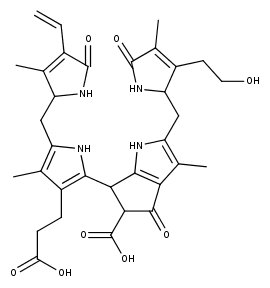
\includegraphics[width=\textwidth]{figures/Kapitel4/Kataboliten/fragmentation_structures/VWA_Katabolit_619.png}
    \caption{}
    \label{fig:619MKLeafspraystructure}
  \end{subfigure}
  \hfill
  \begin{subfigure}[b]{0.5\textwidth}
    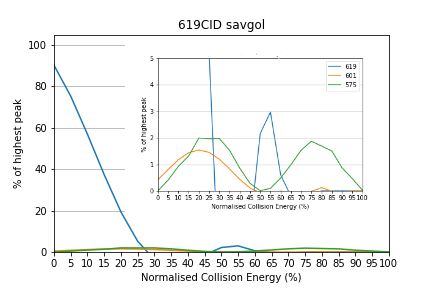
\includegraphics[width=\textwidth]{figures/Kapitel4/Kataboliten/diags/619CID-savgol.png}
    \caption{}
    \label{fig:619MKLeafspraydiags}
  \end{subfigure}
  \caption[Strukturvorschlag von Bo-DNCC mit Fragmentierungsdiagramm, Quelle: Author]{(a) Struktur von Bo-DNCC mit Summenformel \ch{C33H38N4O8}, (b) Fragmentierungsdiagramm von Bo-DNCC (blau = 619 [M+H]\textsuperscript{+}, orange = 601 [M - \ch{H2O} + H]\textsuperscript{+}, grün = 575 [M - \ch{H2O} + H]\textsuperscript{+})}
\end{figure}

 Die \ch{H2O} Abspaltung beim Bo-DNCC erreicht ein lokales Maximum bei 20 \gls{nKE} und erfolgt damit im Vergleich zum Bo-NCC-1 und Bo-NCC-3 bei der höchsten \gls{nKE}. Die Abspaltung von \ch{CO2} weist beim Bo-DNCC zwei lokale Maxima, bei 25 \gls{nKE} und 75 \gls{nKE} auf. Das lokale Maximum an der Stelle 75 \gls{nKE} ist dabei etwas weniger intensiv ausgeprägt wie jenes an der Stelle 25 \gls{nKE}. Das erste lokale Maximum befindet sich damit an der gleichen Stelle wie bei Bo-NCC-1 und Bo-NCC-3 (Abbildungen \ref{fig:831MKLeafspraydiags} und \ref{fig:685MKLeafspraydiags}). Das zweite Maximum kann noch nicht geklärt werden, da es bei den anderen bisher analysierten Kataboliten auch nicht beobachtet wurde.

\section{Identifikation der Reaktionsprodukte} \label{sec:RPMSLeafspray}

Für den Nachweis des Stattfindens der Reaktion der \gls{Chl-K}en mit Essigsäureanhydrid, wurde der gleiche Versuchsaufbau wie in Kapitel \ref{sec:Versuchsaufbau} beschrieben, verwendet. Das Anhydrid als Reaktionsprodukt konnte durch Verwendung von Acetonitril als \gls{lm} isoliert werden. Um eine bessere Identifikation der Reaktionsprodukte zu erreichen, wurden Fragmentierungsdiagramme erstellt.  

\subsection{Reaktionsprodukt von Bo-DNCC}

Das Reaktionsprodukt von Bo-DNCC konnte mit m/z = 699 [M+K]\textsuperscript{+} bestimmt werden (Strukturvorschlag - Abbildung \ref{fig:699MKstructure}). Identifiziert wurde es über die charakteristische Abspaltung von Essigsäure (M = 60 Da) bei m/z = 639 [M - \ch{CH3COOH} + K]\textsuperscript{+}. Ein Mechanismus für die Abspaltung wird in Abbildung \ref{fig:699MKelectronMovement} vorgeschlagen. Dieser Mechanismus ähnelt dem Mechanismus der Abspaltung von \gls{meoh} (\gls{zB} beobachtbar bei einem Cj-NCC), wie in \cite{StructureElucidation} publiziert.\\

\begin{figure}[!htbp]
  \centering
  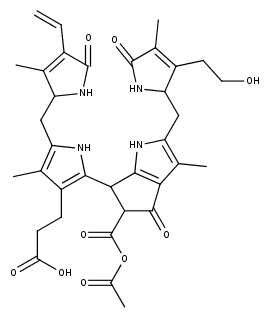
\includegraphics[scale=0.6]{figures/Kapitel4/Kataboliten/fragmentation_structures/VWA_Katabolit_699.png}
  \caption[Strukturvorschlag des Reaktionsproduktes von Bo-DNCC, Quelle: Autor]{Strukturvorschlag des Reaktionsproduktes mit Summenformel \ch{C35H41N4O9}}
  \label{fig:699MKstructure}
\end{figure}

Es wurden Abspaltungen von \ch{H2O} bei m/z = 681 [M - \ch{H2O} + K]\textsuperscript{+}, von \ch{CH3COOH} bei m/z = 639 [M - \ch{CH3COOH} + K]\textsuperscript{+} und von Ring A und Ring D mit \ch{CO2} bei m/z = 311 [M - (Ring A, Ring D, \ch{CO2}) + K]\textsuperscript{+} beobachtet. 

Zur Identifikation der Reaktionsprodukte wurde die \ch{CH3COOH} Abspaltung aufgrund ihrer Dominanz und Eindeutigkeit herangezogen (\gls{uA} Abbildung \ref{fig:699MKstructurediags2}). Das Fragment bei m/z = 599 [M - (\gls{nAb}) + K]\textsuperscript{+} ist interessant, da eine Abspaltung von 100 Da bei anderen Kataboliten ebenfalls beobachtet wurde. Die anderen Fragmentierungen in Abbildung \ref{fig:699MKLeafspray} konnten nicht zugeordnet werden. \\

\begin{figure}[!htbp]
  \centering
  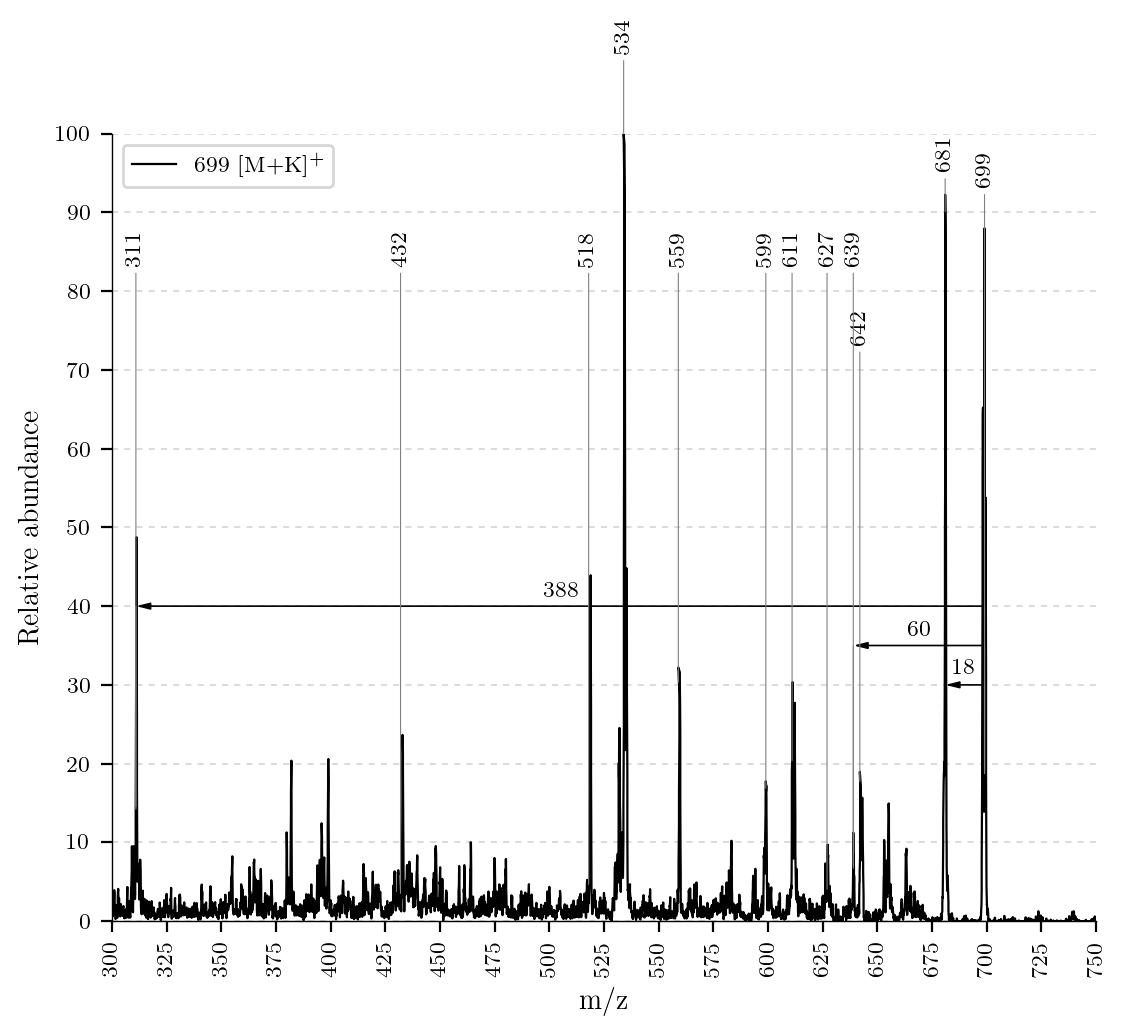
\includegraphics[width=\textwidth, height=0.6\textwidth]{figures/Kapitel4/Kataboliten/VWA_MS_LeafSpray_699.png}
  \caption[ESI-MS Spektrum des Reaktionsproduktes von Bo-DNCC, Quelle: Autor]{ESI-MS Spektrum des Reaktionsproduktes mit m/z = 699 [M+K]\textsuperscript{+}}
  \label{fig:699MKLeafspray}
\end{figure}

Diskussion der Abspaltung bei m/z = 599 [M - (\gls{nAb}) + K]\textsuperscript{+}: Die Abspaltung von 100 Da bei m/z = 599 [M - (\gls{nAb}) + K]\textsuperscript{+} erreicht im Fragmentierungsdiagramm lokale Maxima bei 15 \gls{nKE} und 30 \gls{nKE}. Lokale Minima befinden sich bei 17 \gls{nKE} und 40 \gls{nKE}, an jenen Stellen, an der die Abspaltung von \ch{CH3COOH} lokale Maxima aufweist (Abbildung \ref{fig:699MKstructurediags2}). Daraus könnte man Informationen über den Mechanismus der Abspaltung ableiten. Man könnte sagen, dass die Abspaltung von 100 Da einhergeht mit jener von \ch{CH3COOH} und dass sie mechanistisch miteinander verknüpft sind, also, dass bevor einer Abspaltung des Fragments mit 100 Da \ch{CH3COOH} abgespalten werden muss. Es ließe sich damit erklären, warum bei einem Maximum der einen Abspaltung die andere Abspaltung ein Minimum aufweist.\\ 


\begin{figure}[!htbp]
  \begin{subfigure}[b]{0.5\textwidth}
    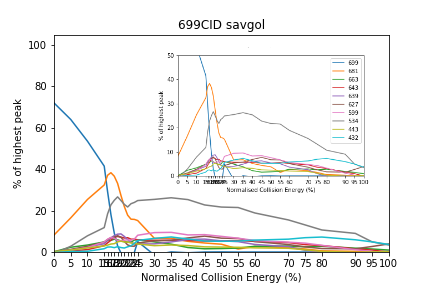
\includegraphics[width=\textwidth, height=\textwidth]{figures/Kapitel4/Kataboliten/diags/699CID-savgol2.png}
    \caption{}
    \label{fig:699MKLeafspraydiags1}
  \end{subfigure}
  \hfill
  \begin{subfigure}[b]{0.5\textwidth}
    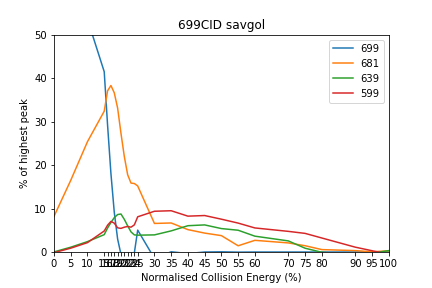
\includegraphics[width=\textwidth, height=\textwidth]{figures/Kapitel4/Kataboliten/diags/699CID-savgol1.png}
    \caption{}
    \label{fig:699MKstructurediags2}
  \end{subfigure}
  
  \caption[Fragmentierungsdiagramme des Reaktionsproduktes von Bo-DNCC, Quelle: Autor]{(a) Fragmentierungsdiagramm des Bo-NCC-3 mit allen beobachteten Abspaltungen (blau = 699 [M+K]\textsuperscript{+}, orange = 681 [M - \ch{H2O} + K]\textsuperscript{+}, grün = 663 [M - (2x\ch{H2O}) + K]\textsuperscript{+}, rot = 643 [M - (\gls{nAb}) + K]\textsuperscript{+}, violett = 639 [M - \ch{CH3COOH} + K]\textsuperscript{+}, braun = 627 [M - (\gls{nAb}) + K]\textsuperscript{+}, pink = 599 [M - (\gls{nAb}) + K]\textsuperscript{+}, grau = 534 [M - (\gls{nAb}) + K]\textsuperscript{+}, hellgrün = 443 [M - (\gls{nAb}) + K]\textsuperscript{+}, türkis = 432 [M - (\gls{nAb}) + K]\textsuperscript{+}), (b) Fragmentierungsdiagramm mit ausgewählten Abspaltungen (blau = 699 [M+K]\textsuperscript{+}, orange = 681 [M - \ch{H2O} + K -\ch{H2O}, grün = 639 [M - \ch{CH3COOH} + K], rot = 599 [M - (\gls{nAb}) + K]\textsuperscript{+})}
\end{figure} 

Im Fragmentierungsdiagramm erreicht die \ch{H2O} Abspaltung ein lokales Maximum bei 17 \gls{nKE}. Die Abspaltung nimmt bis zu 30 \gls{nKE} stark ab und bleibt bis zu 90 \gls{nKE} erhalten. Im Vergleich zum Fragmentierungsdiagramm des nicht reagierten Bo-DNCC erfolgt die \ch{H2O} Abspaltung bei einer niedrigeren \gls{nKE} und ist länger beobachtbar (vergleiche Abbildungen \ref{fig:619MKLeafspraydiags} und \ref{fig:699MKstructurediags2}). Es gilt zu bedenken, dass beim nicht reagierten Bo-DNCC das [M+H]\textsuperscript{+}-Ion aufgenommen wurde, wohingegen man beim reagierten Bo-DNCC das [M+K]\textsuperscript{+}-Ion analysierte. Der Unterschied im Verlauf der Kurven könnte somit auch durch diesen Umstand hervorgerufen werden.

Die Abspaltung von \ch{CH3COOH} besitzt lokale Maxima bei 20 \gls{nKE} und 45 \gls{nKE}. Das Maximum bei 45 \gls{nKE} ist weniger intensiv. Die Intensität der Abspaltung nimmt dabei kontinuierlich bis zu einer von 80 \gls{nKE} ab (Abbildung \ref{fig:699MKstructurediags2}). Ein lokales Minimum der Abspaltung befindet sich zwischen 23 \gls{nKE} und 30 \gls{nKE}. \\



\begin{figure}[!htbp]
  \begin{subfigure}[b]{0.5\textwidth}
    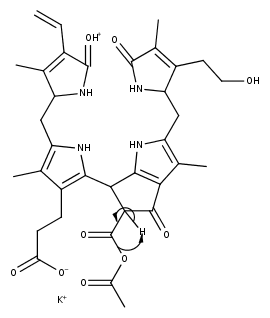
\includegraphics[width=\textwidth, height=\textwidth]{figures/Kapitel4/Kataboliten/fragmentation_structures/VWA_Katabolit_699-639_MK_electronMovement.png}
    \caption{}
    \label{fig:699MKelectronMovement}
  \end{subfigure}
  \hfill
  \begin{subfigure}[b]{0.5\textwidth}
    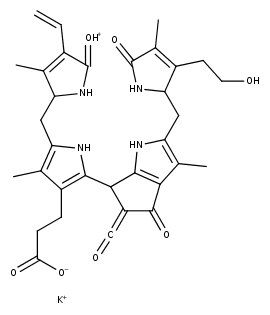
\includegraphics[width=\textwidth, height=\textwidth]{figures/Kapitel4/Kataboliten/fragmentation_structures/VWA_Katabolit_699-639_MK.png}
    \caption{}
    \label{fig:699MK639}
  \end{subfigure}
  \caption[Vorschlag des Mechanismus der \ch{CH3COOH} Abspaltung, Quelle: Autor]{(a) vorgeschlagener Mechanismus der Essigsäureabspaltung und (b) das Produkt, wobei \ch{CH3COOH} als stabiles Neutralteilchen abgespalten wird}
\end{figure}



\pagebreak
\subsection{Reaktionsprodukt von Bo-NCC-3}

Die Molekülmasse des Reaktionsproduktes von Bo-NCC-3 konnte mit m/z = 727 [M+K]\textsuperscript{+} bestimmt werden. Eine Abspaltung von Essigsäure wurde bei m/z = 667 [M+K]\textsuperscript{+} beobachtet. Weiters wurde eine Abspaltung von \ch{H2O} bei m/z = 709 [M - \ch{H2O} + K]\textsuperscript{+} beobachtet. Bei der Abspaltung bei m/z = 627 [M - (\gls{nAb}) + K]\textsuperscript{+} könnte es sich um die gleiche Abspaltung wie beim Reaktionsprodukt des Bo-DNCC handeln, da auch ein Fragment mit M = 100 Da abgespalten wird. Die anderen Abspaltungen (Abbildung \ref{fig:727MKLeafspray}) konnten nicht eindeutig zugeordnet werden.

\begin{figure}[!htbp]
  \centering
  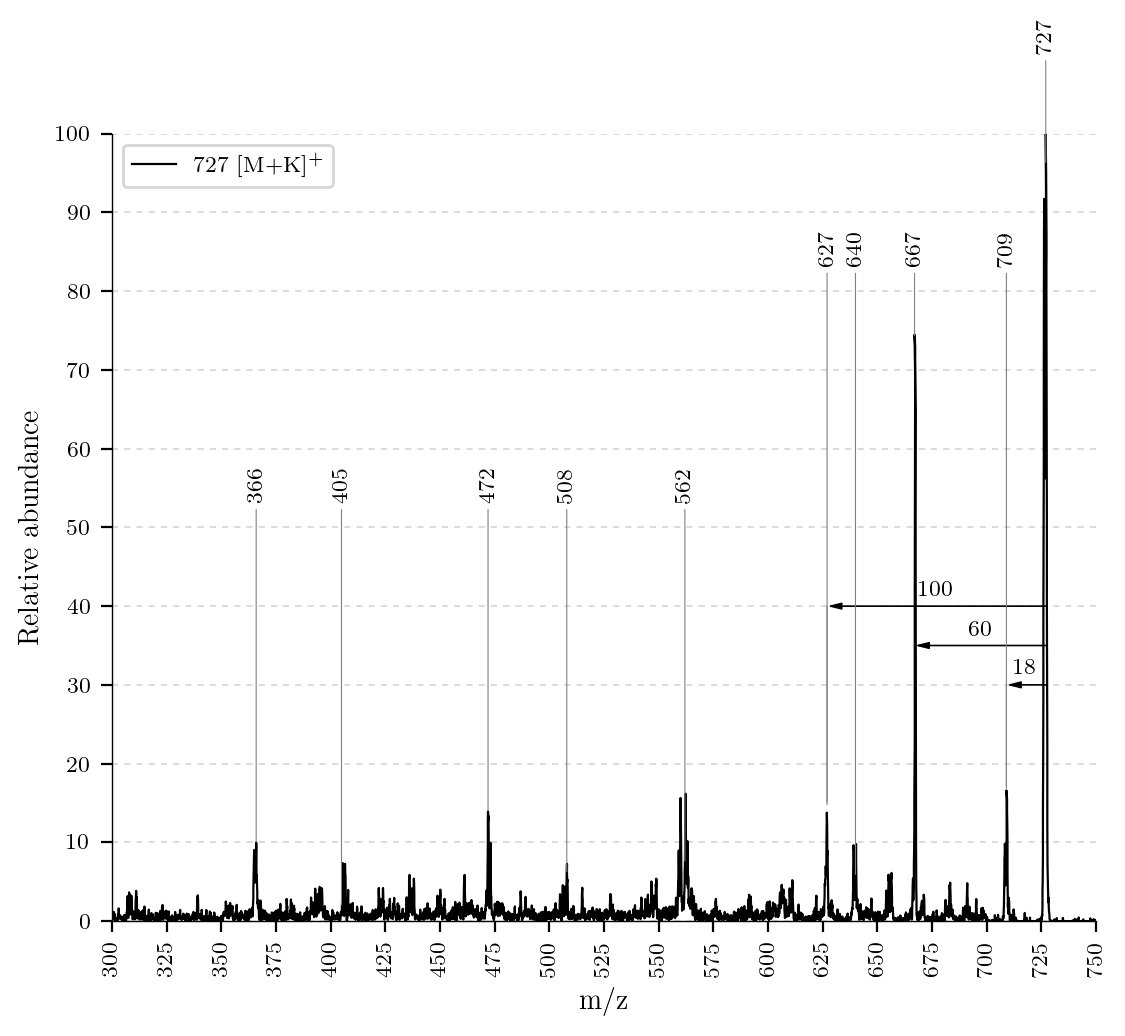
\includegraphics[width=\textwidth, height=0.7\textwidth]{figures/Kapitel4/Kataboliten/VWA_MS_LeafSpray_727.png}
  \caption[ESI-MS des Reaktionsproduktes von Bo-NCC-3, Quelle: Autor]{ESI-MS Spektrum des Reaktionsproduktes bei m/z = 727 [M+K]\textsuperscript{+}}
  \label{fig:727MKLeafspray}
\end{figure}

\begin{figure}[!htbp]
  \centering
  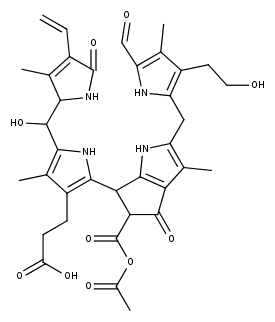
\includegraphics[scale=0.6]{figures/Kapitel4/Kataboliten/fragmentation_structures/VWA_Katabolit_727.png}
  \caption[Strukturvorschlag des Reaktionsproduktes von Bo-NCC-3, Quelle: Autor]{Strukturvorschlag des Reaktionsproduktes mit Summenformel \ch{C36H40N4O10}}
  \label{fig:727MKstructure}
\end{figure}

Es wurde beobachtet, dass die Abspaltung von \ch{H2O} bei niedrigeren Energien erfolgt wie jene von \ch{CH3COOH}. Im Vergleich zum Fragmentierungsdiagramm des Reaktionsproduktes des Bo-DNCC (Abbildung \ref{fig:699MKLeafspraydiags1}) kann als Charakteristikum der \ch{CH3COOH} Abspaltung ein lokales Maximum bei 45 \gls{nKE} gedeutet werden (Abbildung \ref{fig:699MKstructurediags2} und Abbildung \ref{fig:727MKLeafspraydiags}). Die Abspaltung von \ch{H2O} weist bei beiden Kataboliten ein lokales Maximum bei 15 \gls{nKE} auf und besitzt einen ähnlichen Kurvenverlauf (Abbildung \ref{fig:699MKstructurediags2} und Abbildung \ref{fig:727MKLeafspraydiags}). Dies lässt darauf schließen, dass es sich bei dieser \ch{H2O}-Abspaltung um eine Abspaltung auf ein und dersselben Position handelt. Als Position der Abspaltung wird die Hydroxygruppe an Position 32 des Chl-Kataboliten vorgeschlagen. 

\begin{figure}[!htbp]
  \centering
  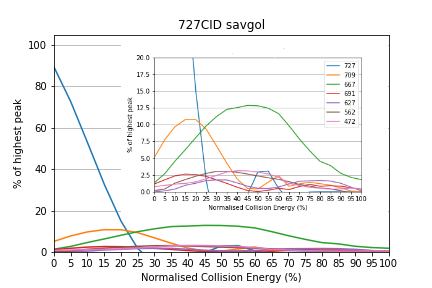
\includegraphics[scale=0.7]{figures/Kapitel4/Kataboliten/diags/727CID-savgol.png}
  \caption[Fragmentierungsdiagramm des Reaktionsproduktes von Bo-DNCC, Quelle: Autor]{Fragmentierungsdiagramm des Reaktionsproduktes (lbau = 727 [M+K]\textsuperscript{+}, orange = 709 [M - \ch{H2O} + K]\textsuperscript{+}, grün = 667 [M - \ch{CH3COOH} + K]\textsuperscript{+}, rot = 691 [M - ? + K]\textsuperscript{+}, violett = 627 [M - ? + K]\textsuperscript{+}, braun = 562 [M - ? + K]\textsuperscript{+}, pink = 472 [M - ? + K]\textsuperscript{+})}
  \label{fig:727MKLeafspraydiags}
\end{figure}



\subsection{Reaktionsprodukt von Bo-NCC-1}

Erwartungsgemäß konnte das Reaktionsprodukt des Bo-NCC-1 bei m/z = 873 [M+K]\textsuperscript{+} gefunden werden. Es zeigt Abspaltungen von \ch{H2O} bei m/z = 855 [M - \ch{H2O} + K]\textsuperscript{+}, von Essigsäure bei m/z = 813 [M - \ch{CH3COOH} + K]\textsuperscript{+}und von \ch{CH3COOH}, Ring A, Ring D, zweimal \gls{meoh} und \ch{CO} bei m/z = 309 [M - (Ring A, Ring D, 2mal MeOH, \ch{CO})  + K]\textsuperscript{+} (diesselbe Abspaltung wurde beim Reaktionsprodukt m/z = 661 [M+H]\textsuperscript{+} beobachtet - Kapitel \ref{sec:ESIMSRPBoNCC3}). Beim Fragment m/z = 441 [M - (Ring D, 2mal MeOH, \ch{H2O}) + K]\textsuperscript{+} könnte es sich um eine Abspaltung von Ring D, zweimal \gls{meoh} und \ch{H2O} handeln. 

\begin{figure}[htbp]
  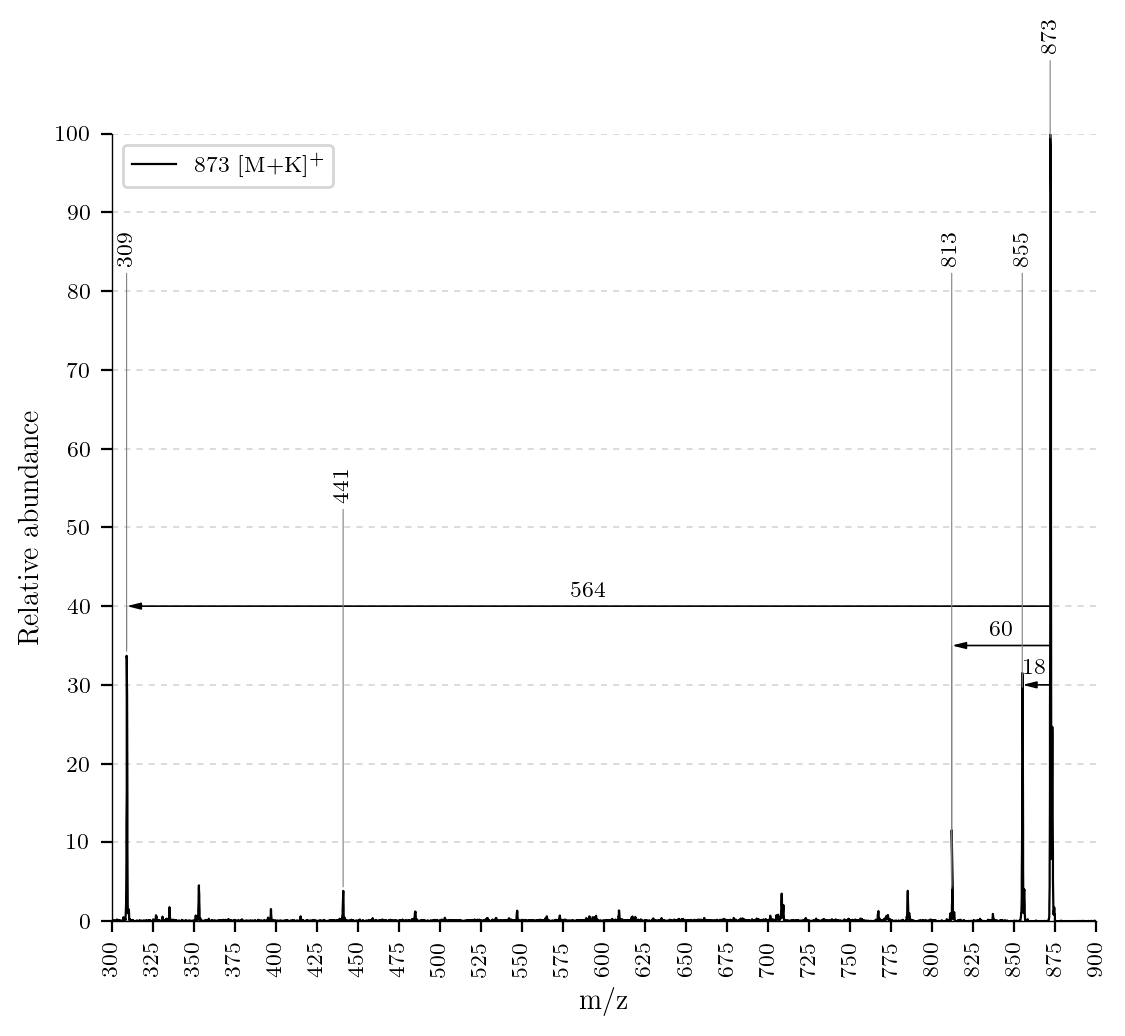
\includegraphics[width=\textwidth, height=0.7\textwidth]{figures/Kapitel4/Kataboliten/VWA_MS_LeafSpray_873.png} 
  \caption[ESI-MS des Reaktionsproduktes von Bo-NCC-1, Quelle: Autor]{ESI-MS des Reaktionsproduktes bei m/z = 873 [M+K]\textsuperscript{+}}
  \label{fig:873MKLeafspray}
\end{figure}

\begin{figure}[htbp]
  \centering
  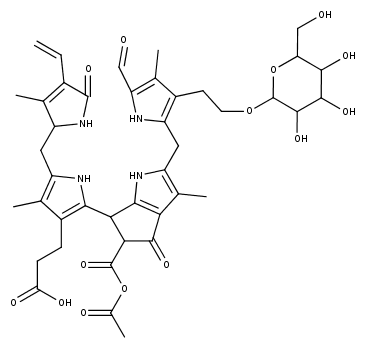
\includegraphics[scale=0.6]{figures/Kapitel4/Kataboliten/fragmentation_structures/VWA_Katabolit_873.png}
  \caption[Strukturvorschlag des Reaktionsproduktes von Bo-NCC-1, Quelle: Autor]{Strukturvorschlag des Reaktionsproduktes mit Summenformel \ch{C42H50N4O14}}
  \label{fig:873MKstructure}
\end{figure}

Im Fragmentierungsdiagramm sieht man, dass sich das lokale Maximum der Essigsäureabspaltung hin zu niedrigeren Energien verschoben hat. Es befindet sich nun bei  35 \gls{nKE}. Auch die \ch{H2O} Abspaltung verschiebt sich zu niedrigeren Energien und besitzt ein lokales Maximum bei 10 \gls{nKE}. Im Vergleich zum Bo-DNCC und Bo-NCC-3 nahmen diese Werte um 10 bzw. 5 Einheiten an \gls{nKE} ab. Dieser Zusammenhang wurde in zwei voneinander unabhängigen Experimenten beobachtet (Abbildung \ref{fig:873MKLeafspraydiags1} und Abbildung \ref{fig:873MKstructurediags2}). Die Ursache könnte beim Zuckerring liegen, der die Elektronenverteilung vermutlich so beeinflusst, dass die Abspaltungen bereits bei niedrigeren Energien erfolgen. 

(Einfügen von 3D Bildern, die die sterischen Zusammenhänge vorschlagen).

\begin{figure}[!htbp]
  \begin{subfigure}[b]{0.5\textwidth}
    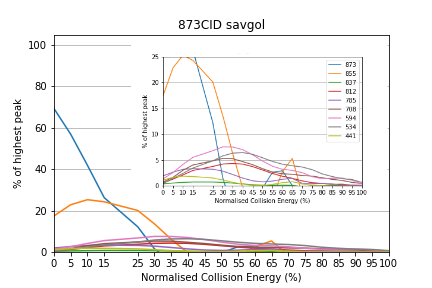
\includegraphics[width=\textwidth, height=\textwidth]{figures/Kapitel4/Kataboliten/diags/873CID-savgol1.png}
    \caption{}
    \label{fig:873MKLeafspraydiags1}
  \end{subfigure}
  \hfill
  \begin{subfigure}[b]{0.5\textwidth}
    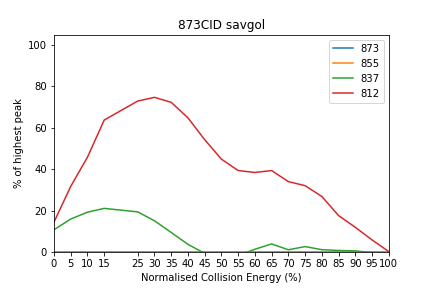
\includegraphics[width=\textwidth, height=\textwidth]{figures/Kapitel4/Kataboliten/diags/873CID-savgol2.png}
    \caption{}
    \label{fig:873MKstructurediags2}
  \end{subfigure}
  
  \caption[Fragmentierungsdiagramm des Reaktionsproduktes von Bo-NCC-1, Quelle: Autor]{Fragmentierungsdiagramm des Reaktionsproduktes: (a) Experiment am 13.09.2017 (11:00) - (blau = 873, orange = 855, grün = 837, rot = 812, violett = 765, braun = 708, pink = 594, grau = 534, hellgrün = 441), (b) Experiment am 13.09.2017 (09:45) - schlechter gelungen, weswegen die Abspaltungen nicht so schön wie in Experiment (a) zu sehen sind (blau = 873, orange = 855, grün = 837, rot = 812}
\end{figure}
\chapter{Experimente LC-MS} 

Die Analyse mit \gls{lcms} diente dazu, die Ergebnisse von MS Leafspray zu überprüfen. In Kombination mit einem hochauflösenden Massenspektrometer wurde zudem die Ermittlung der Strukturen der \gls{Chl-K}en erleichtert. Weiters konnten mit MS Leafspray nicht gefundene \gls{Chl-K}en identifiziert werden. \\

\section{HPLC-Gradient und Gerätebeschreibungen} \label{sec:HPLCAufarbeitungderProbe} 

Als Massenspektrometer wurde ein Thermo LTQ Orbitrap XL im positiven Ionenmodus verwendet (3-6 kV Sprayspannung, m/z von 300 - 1000). Dieses wurde auch für die Messungen von Kapitel \ref{sec:ChlKatabolitenESIMS} verwendet.

\section{Aufarbeitung der Probe} \label{sec:HPLCAufarbeitungderProbe}

Um ein Blattextrakt zu erhalten, wurde ein Brokkoliblatt auf eine Größe von \gls{ca} 2 \si{cm^{2}} mit einer Rasierklinge zugeschnitten, mithilfe von Mörser und Pistill aufgerieben und mit 2-5 mL \gls{meoh} vermengt (Anm.: um möglichst hohe Intensitäten in der \gls{hplc} zu erhalten wurde versucht, eine möglichst hohe Konzentration des Blattextraktes zu erreichen). Die Lösung wurde für 2 min. bei 3000 rpm abzentrifugiert und anschließend mit Wasser im Verhätnis 20:80 verdünnt und nach kurzem Homogenisieren für 7 min. (3000 rpm) abzentrifugiert. Von der erhaltenen Lösung wurden 50 \si{\uL} in die 20 \si{\uL} Schleife der \gls{hplc} eingespritzt. 

%Da beobachtet wurde, dass die erhaltene Lösung nach der beschriebenen Aufarbeitung nicht homogen ist, wurde versucht, sie mithilfe von Filterpapier zu filtern. Es zeigte sich jedoch, dass dies die Intensitäten in der \gls{hplc} stark reduziert (siehe Anhang), weswegen die oben beschriebene Aufarbeitung beibehalten wurde.

Beim Einspritzen wurde versucht, die ungelösten Bestandteile im Blattextrakt nicht mitzunehmen, da diese die \gls{hplc} mit der Zeit verunreinigen könnten. Eine Filterung des Blattextraktes erwies sich als Intensitätsverringernd.

Bevor die Blätter wie oben beschrieben aufgerieben wurden, wurden sie in einem Exikator getrocknet (ca. einen halben bis ganzen Tag). Die Blätter, an denen die Reaktion (Kapitel \ref{sec:ReaktionEssig}) stattgefunden hatte, wurden nach dem Stoppen der Reaktion der gleichen Aufarbeitungsmethode unterzogen. 

\section{Theoretische Auswertung der Online-UV/Vis Spektren} \label{sec:IdentifikationUVVis}

Mithilfe einer HPLC kann bestimmt werden, ob es sich bei einem bestimmten \gls{Chl-K}en um einen \gls{NCC}, \gls{DNCC} oder \gls{YCC} handelt. Man erhält zu jedem Peak im \gls{hplc} Chromatogramm ein Online-UV/Vis Spektrum, das von einem an die \gls{hplc} angeschlossenen UV/Vis Detektor gemessen wurde (Kapitel \ref{sec:HPLCAufarbeitungderProbe}). \\

Ein \gls{NCC} kann über eine charakteristische Bande bei 315 nm eindeutig bestimmt werden. Die Bande geht dabei auf das konjugierte System von Ring A zurück. Ein \gls{DNCC} besitzt aufgrund seiner decarboxylierten Carbonylgruppe dieses konjugierte System nicht mehr, weswegen die Bande bei 315 nm verschwindet, der sonstige für einen \gls{NCC} typische Kurvenverlauf jedoch erhalten bleibt. Bei einem \gls{YCC} führt die Reduktion der Verbindung zwischen Ring C und D (Einführung einer Doppelbindung zwischen Position 15 und 16) zu einer Erweiterung des konjugierten Systems (nun bestehend aus Ring C und D) und damit zu einer Bande bei 415 nm. \\

Alle folgenden UV/Vis Spektren und \gls{hplc} Chromatogramme wurden bei 254 nm detektiert.

\section{Theoretische Auswertung der MS Spektren} \label{sec:IdentifikationMS}

̈Über das an die HPLC gekoppelte Massenspektrometer wird zu jedem Zeitpunkt des \gls{hplc} Chromatogramms ein Massenspektrum aufgenommen und ein dementsprechendes Chromatogramm erzeugt. Die hervorgehobenen Peaks in den folgenden Chromatogrammen zeigen an, zu welchem Zeitpunkt welcher Katabolit in Bezug auf seine Molekülmasse gefunden wurde. Da das Massenspektrometer erst nach 10 min. an die HPLC gekoppelt wurde, muss man, um die entsprechende Retentionszeit im HPLC Chromatogramm zu erhalten, zu jedem Zeitpunkt im Chromatogramm des Massenspektrometers ca. 11 min. dazuzählen (1 min. steht für den Weg von HPLC zu MS).  \\

Man kann somit den über Online-UV/Vis Spektren identifizierten \gls{Chl-K}en (Kapitel \ref{sec:IdentifikationUVVis}) eine Molekülmasse zuordnen. Im Rahmen meiner Vorwissenschaftlichen Arbeit erwies es sich jedoch als schwierig, die Resultate der \gls{hplc} mit denen des Massenspektrometers im Rahmen eines \gls{lcms} Versuches in Einklang zu bringen (die Retentionszeiten der über \gls{hplc} identifizierten \gls{Chl-K}en stimmten mit jenen des Massenspektrometers oft nicht überein). Da die Verwendung von Daten aus der \gls{hplc} zur Analyse der \gls{Chl-K}en nicht das primäre Ziel meiner Arbeit war, spielt dies auch keine wesentliche Rolle. Aus Gründen der wissenschaftlichen Vollständigkeit, werden die Daten der \gls{hplc} trotzdem präsentiert. Ebenso wird versucht, die Probleme, die sich aus den Daten ergeben, darzustellen.\\

Der Typ des \gls{Chl-K}en wurde somit, sofern möglich durch ein Online-UV/Vis Spektrum bestimmt und mit der vom Massenspektrometer erhaltenen Summenformel und den sich daraus ergebenden strukturellen Möglichkeiten überprüft. War die Zuordnung anhand UV/Vis Spektren aufgrund von Unklarheiten nicht möglich, wurde zur Strukturbestimmung auf die Daten des Massenspektrometers zurückgegriffen.\\

\section{Chl-Kataboliten des Brokkoliblattes mithilfe von LC-MS identifiziert} \label{sec:ChlKatabolitenBrokkoli}

Das HPLC Chromatogramm in Abbildung \ref{fig:HPLCChromatogramm} zeigt, welche der Kataboliten mithilfe ihrer UV/Vis Spektren eindeutig identifiziert werden konnten. Es dürfte sich dabei ob ihrer etwas höheren Intensitäten um die Hauptkataboliten des Brokkoliblattes handeln. Dies müsste jedoch in gezielten quantitativen Messungen weiter und genauer untersucht werden.

\begin{figure}[!htbp]
  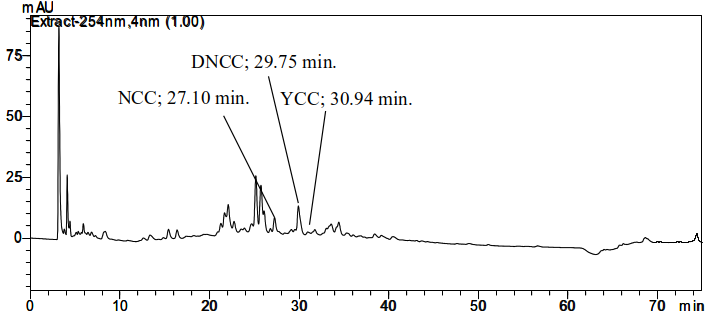
\includegraphics[width=\textwidth]{figures/Kapitel6/keineReaktion/VWA_HPLC_Chromatogramm_keineReaktion.png}
  \caption[HPLC Chromatogramm vor der Reaktion, Quelle: Autor]{\gls{hplc} Chromatogramm - die hervorgehobenen Peaks entsprechen den Retentionszeiten und der Art der \gls{Chl-K}en, die über ein Online-UV/Vis Spektrum bestimmt wurden; gefunden wurden ein \gls{NCC} bei 27.10 min. (Abbildung \ref{fig:NCC2725}), ein DNCC bei 29.75 min. (Abbildung \ref{fig:DNCC2991}) und ein YCC bei 30.94 min. (Abbildung \ref{fig:YCC3094})}
  \label{fig:HPLCChromatogramm}
\end{figure}

\begin{figure}[!htbp]
  \centering
  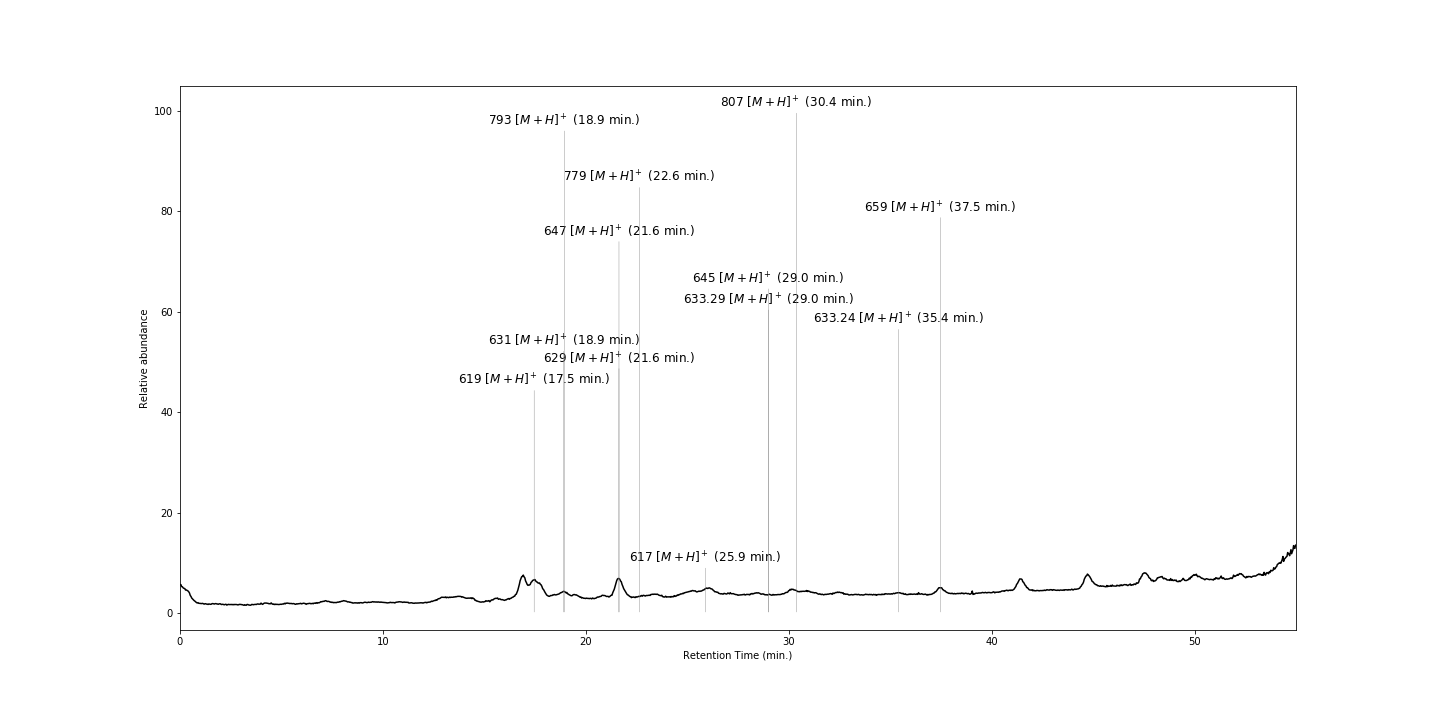
\includegraphics[width=1.4\textwidth, center]{figures/Kapitel6/keineReaktion/Kuerbis_Analyse_keineReaktion2_Ganzes_Spektrum.png}
  \caption[LC-MS Chromatogramm vor der Reaktion, Quelle: Autor]{\gls{lcms} Chromatogramm}
  \label{fig:LCMSChromatogramm}
\end{figure}

Mit dem Massenspektrometer wurden die in Tabelle \ref{tab:LCMSKataboliten} aufgelisteten Phyllobiline identifiziert. In dieser Tabelle werden neben den Summenformeln auch die exakten Molekülmassen (in Da), die Art des \gls{Chl-K} (NCC, DNCC, YCC, DYCC) und die Retentionszeit in der \gls{hplc} (soweit eindeutig feststellbar) angegeben. \\

Eine so große Anzahl an \gls{Chl-K}en wie in Tabelle \ref{tab:LCMSKataboliten} vorzufinden wäre ungewöhnlich. Bei einer Betrachtung der Summenformeln und exakten Molekülmassen fällt jedoch auf, dass sich einige \gls{Chl-K}en um genau ein C-Atom und zwei H-Atome unterscheiden (entsprich einem Massenunterschied von 14 Da). 

Da alle identifizierten \gls{Chl-K} eine freie Carbonsäuregruppe an Position 8\textsuperscript{2} besitzen, wird angenommen, dass diese bei der Aufarbeitung der Probe mit \gls{meoh} (Kapitel \ref{sec:HPLCAufarbeitungderProbe}) mit diesem reagieren und einen Methylester ausbilden. In der Spalte Herkunft (abgekürzt mit H.) der Tabelle \ref{tab:LCMSKataboliten} wird demnach festgehalten, von welchem \gls{Chl-K}en die jeweilige Verbindung stammt. Es handelt sich dabei also um keine \gls{Chl-K}en, sondern nur um deren Reaktionsprodukte mit \gls{meoh}. In der \gls{hplc} konnten sie jedoch nicht identifiziert werden. \\

\begin{table*}\centering
  \ra{1.3}

  \begin{tabular}{cccccc}\toprule
 Bezeichnung & Summenformel & M (in Da) & Typ & RT\textsubscript{HPLC} (in min.) & H. \\
\midrule
\rowcolor{black!20} Bo-DYCC & \ch{C33H37O8N4} & 617.2635 & DYCC & 30.94? & - \\
 Bo-DNCC & \ch{C33H39O8N4} & 619.2793 & DNCC & 26.72 & - \\ 
\rowcolor{black!20} • & \ch{C34H37O8N4} & 629.2639 & • & - & - \\ 
 - & \ch{C34H39O8N4} & 631.2795 & DYCC & 29.91, 30.94 & Bo-DYCC \\ 
\rowcolor{black!20} - & \ch{C34H41O8N4} & 633.2955 & DNCC & - & Bo-DNCC \\ 
 • & \ch{C36H33O7N4} & 633.2339 & • & • & - \\ 
\rowcolor{black!20} Bo-YCC & \ch{C34H37O9N4} & 645.2593 & YCC & - & - \\ 
 Bo-NCC-3 & \ch{C34H39O9N4} & 647.2748 & NCC & 33.04 & - \\ 
\rowcolor{black!20} - & \ch{C35H39O9N4} & 659.2741 & YCC & - & Bo-YCC \\
 Bo-DNCC-2 & \ch{C39H47O13N4} & 779.3181 & DNCC & • & - \\ 
\rowcolor{black!20}Bo-NCC-1 & \ch{C40H49O13N4} & 793.3336 & NCC & 29.91 & - \\ 
 - & \ch{C41H51O13N4} & 807.3491 & NCC & - & Bo-NCC-1 \\ 
\bottomrule
  \end{tabular}
  \caption[Übersicht über die Chl-Kataboliten des Brokkoliblattes, Quelle: Autor]{Übersicht über die gefundenen Chl-Kataboliten des Brokkoliblattes und ihren Methylestern, die sich aus der Reaktion der freien Carbonsäure mit \gls{meoh} ergeben (die Summenformeln und die exakten Molekülmassen beziehen sich auf die [M+H]\textsuperscript{+} Ionen)}
  \label{tab:LCMSKataboliten}
\end{table*}

Bei einer Retentionszeit von 27.10 min. konnte über Online-UV/Vis ein \gls{NCC} (Abbildung \ref{fig:NCC2725}) identifiziert werden, da er bei einer Wellenlänge von 315 nm eine charakteristische Bande aufweist. Der von den Retentionszeiten dazugehörige \gls{Chl-K} im Massenspektrum wäre der Bo-DNCC (mit einer Retentionszeit von 17.5 min im Massenspektrometer - Abbildung \ref{fig:LCMSChromatogramm}). Bei diesem handelt es sich jedoch um einen \gls{DNCC}. Es wurde versucht, das unlogische Ergebnis durch Überlagerungen mehrer \gls{Chl-K}en zu erklären, was aber nicht möglich war (Abbildung \ref{fig:LCMSChromatogrammAufspaltung}). Es bleibt somit das Zustandekommen dieses UV/Vis Spektrums ungeklärt. 

Bei einer Retentionszeit von 29.75 min. konnte ein UV/Vis Spektrum eines \gls{DNCC}s (Abbildung \ref{fig:DNCC2991}) aufgenommen werden. Nach den Retentionszeiten im Massenspektrometer (Abbildung \ref{fig:LCMSChromatogramm}) kann diesem UV/Vis Spektrum der \gls{Chl-K} Bo-NCC-1 zugeordnet werden. Auch der Methylester des Bo-YDNCC ist zu dieser Retentionszeit im Massenspektrometer vorzufinden und trägt damit vermutlich zur Entstehung des Signals bei, was die Verzerrungen bewirken könnte (Abbildung \ref{fig:LCMSChromatogrammAufspaltung}).

\begin{figure}[!htbp]
  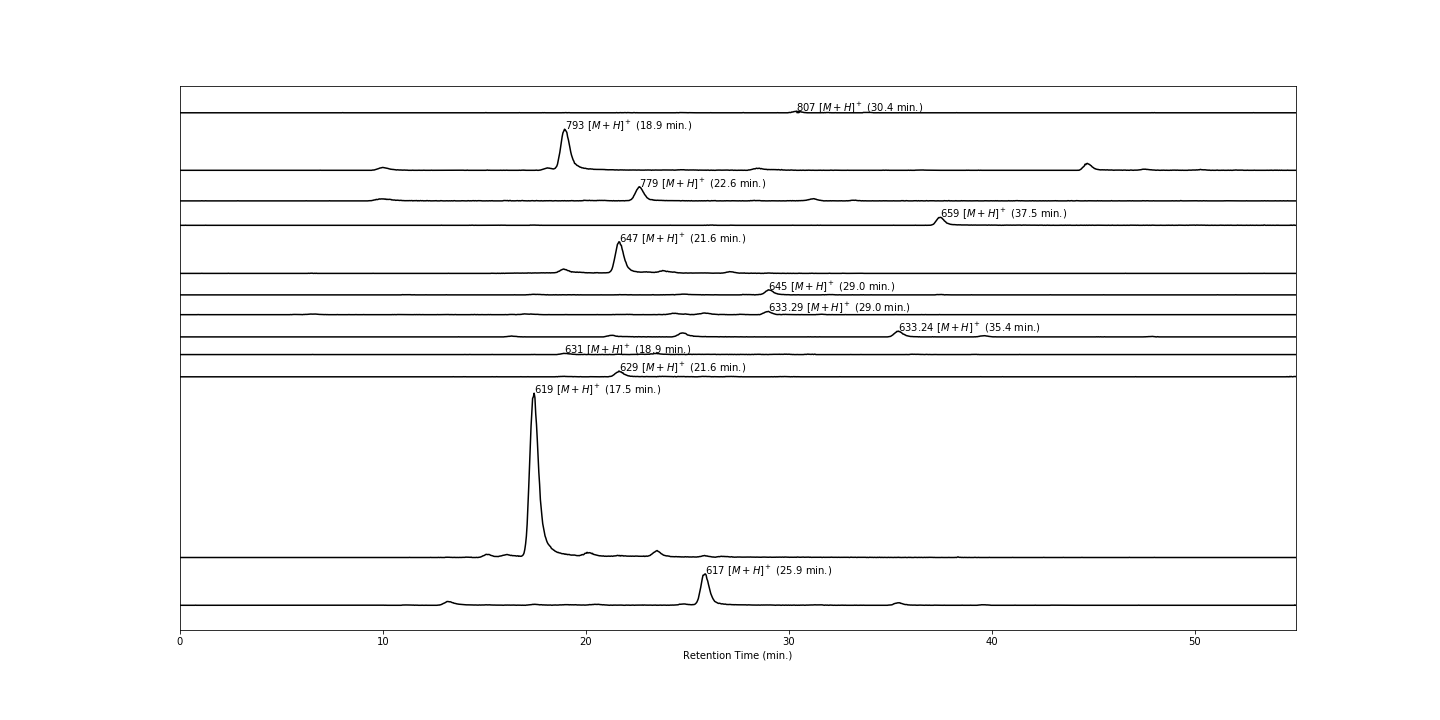
\includegraphics[width=1.4\textwidth, center]{figures/Kapitel6/keineReaktion/Kuerbis_Analyse_keineReaktion2_LC-ESI-MS.png}
  \caption[LC-MS Chromatogramm vor der Reaktion - Aufspaltung der Signale, Quelle: Autor]{\gls{lcms} Chromatogramm zur besseren Darstellung von Überlagerungen von Chlorophyllkataboliten, um diverse unlogische Schlüsse besser verstehen zu können}
  \label{fig:LCMSChromatogrammAufspaltung}
\end{figure}

Bei einer Retentionszeit von 30.94 min. ist das UV/Vis Spektrum charakteristisch für einen \gls{YCC} (Abbildung \ref{fig:DNCC2991}). Im Massenspektrometer wurde zu dieser Retentionszeit der Methylester des Bo-YDNCC gefunden (bei einer Retentionszeit von 18.9 min). Auch hier lässt sich keine Verbindung finden, bei der die Retentionszeiten von \gls{hplc} und Massenspektrometer exakt zusammenpassen. Es könnte auch hier wieder zu einer Überlagerung kommen (vielleicht mit dem Bo-YDNCC). Diese Überlagerungen könnten durch Isomere der einzelnen \gls{Chl-K}en bedingt sein. \\
 

Um das Zustandekommen der nicht identifizierbaren UV/Vis Spektren zu erklären wurden Diagramme wie in Abbildung \ref{fig:LCMSChromatogrammAufspaltung} erstellt. Es handelt sich dabei um ein Chromatogramm jedes einzelnen im Massenspektrometer während eines \gls{lcms} Laufes identifizierten \gls{Chl-K}en. Die Intensitäten wurden auf den höchsten im Zeitraum vorkommenden Peak skaliert. Bei den gekennzeichneten Peaks handelt es sich um jene, bei denen die jeweilige Verbindung die höchste Intensität im Chromatogramm zeigte. Peaks etwaiger Stereoisomere werden nicht beachtet. Mithilfe dieser Abbildung sollten etwaige Überlagerungen ersichtlich werden. 

\begin{figure}[!htbp]
  \begin{subfigure}[b]{0.5\textwidth}
    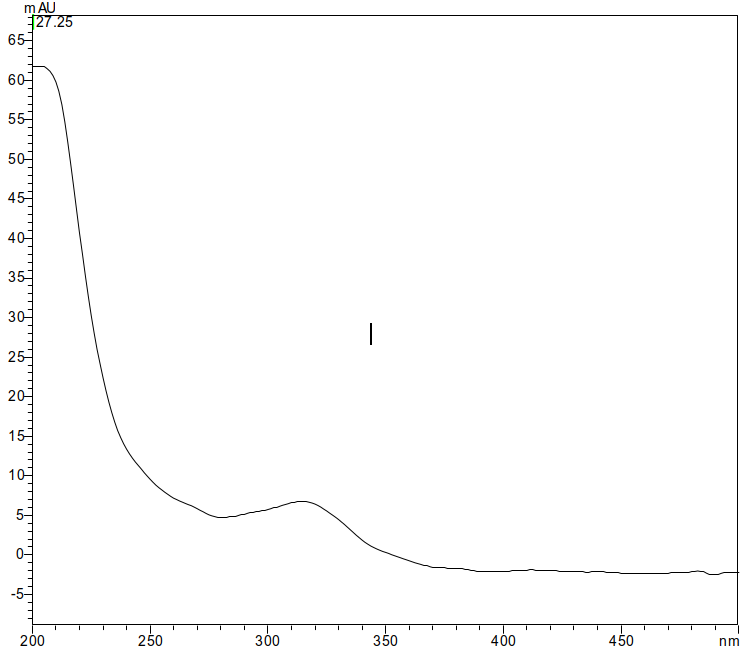
\includegraphics[width=\textwidth]{figures/Kapitel6/keineReaktion/NCC2725.png}
    \caption{}
    \label{fig:NCC2725}
  \end{subfigure}
  \hfill
  \begin{subfigure}[b]{0.5\textwidth}
    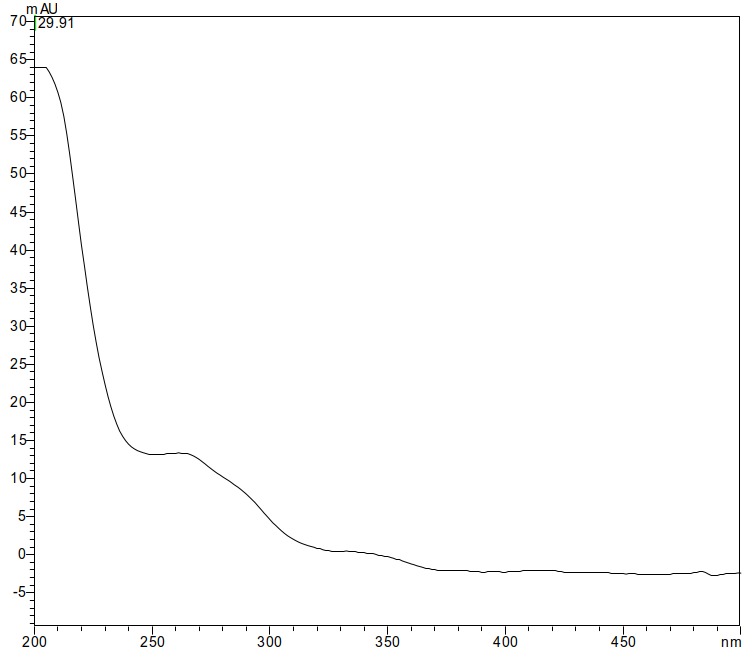
\includegraphics[width=\textwidth]{figures/Kapitel6/keineReaktion/DNCC2991.png}
    \caption{}
    \label{fig:DNCC2991}
  \end{subfigure}
  
  \begin{subfigure}[b]{0.5\textwidth}
    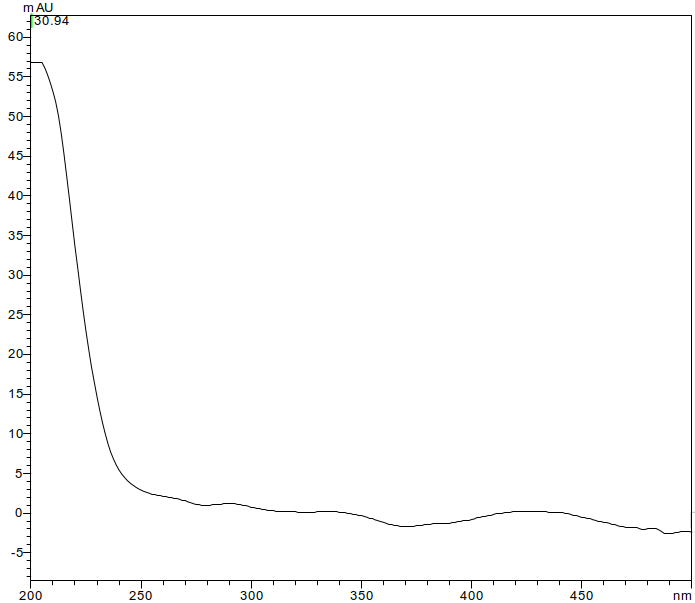
\includegraphics[width=\textwidth]{figures/Kapitel6/keineReaktion/YCC3094.png}
    \caption{}
    \label{fig:YCC3094}
  \end{subfigure}
  \caption[Online-UV/Vis Spektren mit der Charakteristik eines NCC bei 27.10 min., eines DNCC bei 29.75 min. sowie eines YCC bei 30.94 min., Quelle: Autor]{Online-UV/Vis Spektren: (a) charakteristisch für einen \gls{NCC} - RT = 27.25 min., (b) charakteristisch für einen \gls{DNCC} - RT = 29.91 min., (c) charakteristisch für einen \gls{YCC} - RT = 30.94 min.}
\end{figure}

\section{Identifikation der Reaktionsprodukte mithilfe von LC-MS}

Die Produkte der Reaktion mit Essigsäureanhydrid konnten ebenfalls mithilfe von \gls{lcms} identifiziert werden. In Abbildung \ref{fig:HPLCChromatogrammRP} sind die Reaktionsprodukte, die mittels UV/Vis online Spektren identifiziert wurden, dargestellt. Die dazugehörigen UV/Vis Spektren werden in Abbildung \ref{fig:YCC3398}-e dargestellt. Es handelt sich dabei um die Hauptreaktionsprodukte, die dadurch charakterisiert sind, dass sich ihre Retentionszeit nach hinten verschiebt. Sie dürften somit apolarere Eigenschaften besitzen wie die \gls{Chl-K}, was vermutlich durch den Methylester bedingt ist. Über die Verschiebung der Peaks im \gls{hplc} Chromatogramm ist das Stattfinden der Reaktion ersichtlich (vergleiche Abbildung \ref{fig:HPLCChromatogramm} und Abbildung \ref{fig:HPLCChromatogrammRP}). Es konnten mehrere Verbindungen über UV/Vis Spektren beobachtet und identifiziert werden wie bei den anderen \gls{hplc} Läufen.

\begin{figure}[!htbp]
  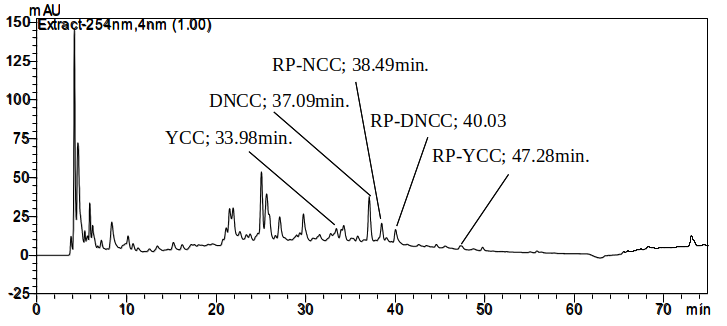
\includegraphics[width=\textwidth]{figures/Kapitel6/Reaktion3h/HPLC_Chromatogramm.png}
  \caption[HPLC Chromatogramm nach 3h Reaktionsdauer, Quelle: Author]{\gls{hplc} Chromatogramm}
  \label{fig:HPLCChromatogrammRP}
\end{figure}

Das Chromatogramm des Massenspektrometers des \gls{lcms} Laufes (Abbildung \ref{fig:LCMSCChromatogrammRP}) zeigt die Massen aller \gls{Chl-K} und die Zeitpunkte, zu denen sie jeweils eluieren. Durch die stattgefundene Reaktion sind dementsprechend mehr Signale vorhanden. Auffallend ist, dass manche Verbindungen in ihren Retentionszeiten verschoben worden sind. So eluiert Verbindung mit m/z = 631 [M+H]\textsuperscript{+} nun bei 39.0min. im Vergleich zu 18.9min., Verbindung mit m/z = 629 [M+H]\textsuperscript{+} bei 31.8min. im Vergleich zu 21.6min. und Verbindung mit m/z = 645 [M+H]\textsuperscript{+} bei 34.5min. im Vergleich zu 29.0min. (vergleiche Abbildung \ref{fig:LCMSCChromatogrammRP} und \ref{fig:LCMSChromatogramm}). Gründe für diese Verschiebung müssten weiter untersucht werden bzw. müsste überprüft werden, ob es bei den Versuchen, aus denen einer zu Abbildung \ref{fig:LCMSChromatogramm} führte, nicht einen Messfehler gab. Eine Überprüfung und erneute Durchführung der Messung führte jedoch zum selben Ergebnis (siehe Anhang).

\begin{figure}[!htbp]
  \centering
  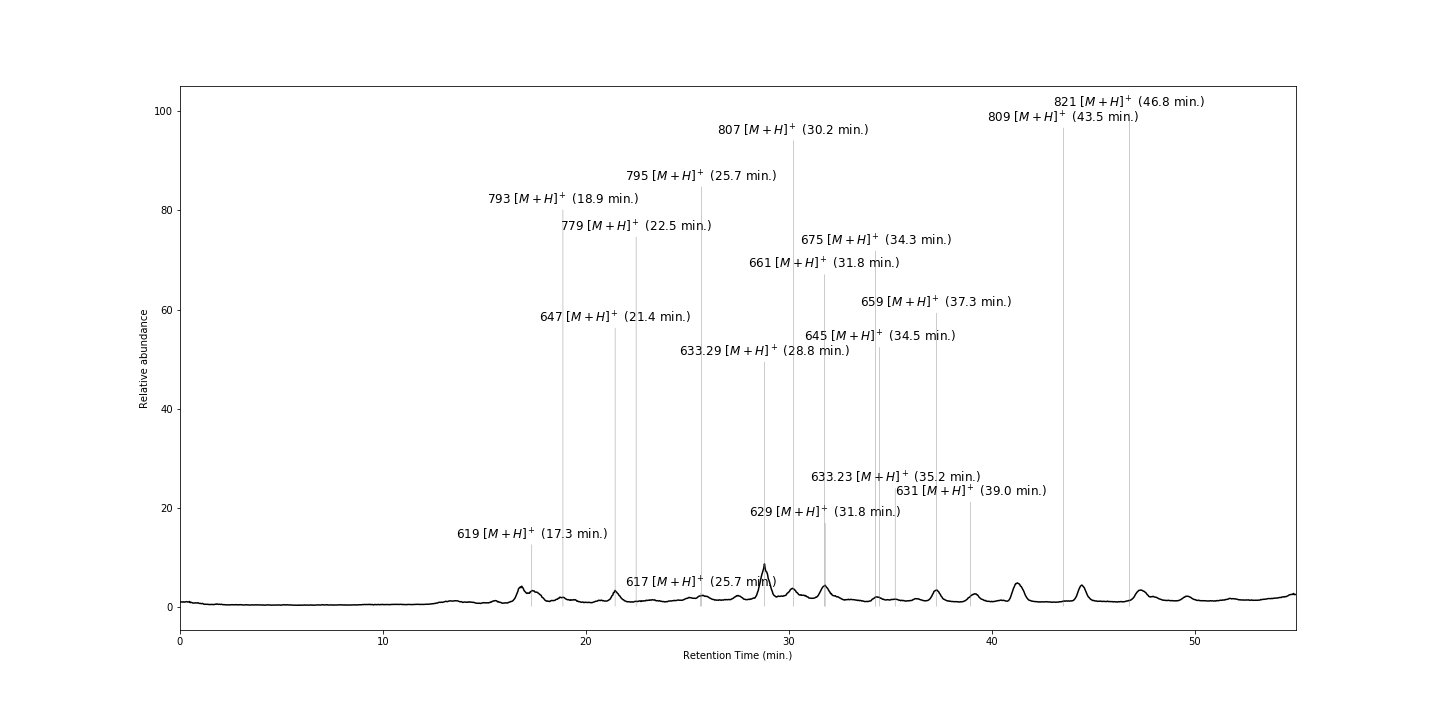
\includegraphics[width=1.1\textwidth]{figures/Kapitel6/Reaktion3h/Kuerbis_Analyse_Reaktion3h_Ganzes_Spektrum.png}
  \caption[LC-MS Chromatogramm nach 3h Reaktionsdauer, Quelle: Author]{\gls{lcms} Chromatogramm}
  \label{fig:LCMSCChromatogrammRP}
\end{figure}

In Tabelle \ref{tab:LCMSKatabolitenRP} werden die \gls{Chl-K} dargestellt, die nach der Reaktion gefunden wurden. Dabei wurden zwei Verbindungen entdeckt, die ähnliche Molekülmassen aufweisen, wie bereits identifizierte, 
\begin{table*}\centering
  \ra{1.3}

  \begin{tabular}{cccccc}\toprule
 Bezeichnung & Summenformel & M (in Da) & Typ & RT\textsubscript{HPLC} (in min.) & H. \\
\midrule
\rowcolor{black!20} Bo-DYCC & \ch{C33H37O8N4} & 617.2599 & DYCC & 30.94? & - \\
 Bo-DNCC & \ch{C33H39O8N4} & 619.2798 & DNCC & 26.72 & - \\ 
\rowcolor{black!20} • & \ch{C34H37O8N4} & 629.2641 & • & - & - \\ 
 - & \ch{C34H39O8N4} & 631.2795 & DYCC & 29.91, 30.94 & Bo-DYCC \\ 
\rowcolor{black!20} - & \ch{C34H41O8N4} & 633.2955 & DNCC & 28.8 & Bo-DNCC \\ 
 • & \ch{C36H33O7N4} & 633.2339 & • & - & - \\ 
\rowcolor{black!20} Bo-YCC & \ch{C34H37O9N4} & 645.2593 & YCC & - & - \\ 
 • & \ch{C35H41O8N4} & 645.2953 & • & - & - \\ 
\rowcolor{black!20} Bo-NCC-3 & \ch{C34H39O9N4} & 647.2748 & NCC & 33.04 & - \\ 
 • & \ch{C34H35O10N4} & 659.2348 & • & - & - \\
\rowcolor{black!20} - & \ch{C35H39O9N4} & 659.2741 & YCC & 37.09 & Bo-YCC \\
 - & \ch{C35H41O9N4} & 661.2902 & - & - & Bo-NCC-3 \\
\rowcolor{black!20} - & \ch{C36H43O9N4} & 675.306 & - & - & Bo-NCC-3 \\
 Bo-DNCC-2 & \ch{C39H47O13N4} & 779.3181 & DNCC & - & - \\ 
\rowcolor{black!20} Bo-NCC-1 & \ch{C40H49O13N4} & 793.3336 & NCC & 29.91 & - \\ 
 - & \ch{C40H51O13N4} & 795.3491 & - & - & - \\ 
\rowcolor{black!20} - & \ch{C41H51O13N4} & 807.3491 & NCC & 40.03 & Bo-NCC-1 \\ 
 - & \ch{C41H53O13N4} & 809.3649 & - & - & 795 \\ 
\rowcolor{black!20} - & \ch{C42H53O13N4} & 821.3652 & NCC & 47.28 & Bo-NCC-1 \\ 
\bottomrule
  \end{tabular}
  \caption[Übersicht über die Chl-Kataboliten des Brokkoliblattes, Quelle: Author]{Übersicht über die gefundenen Chl-Kataboliten des Brokkoliblattes und ihren Methylestern, die sich aus der Reaktion der freien Carbonsäure mit Essigsäureanhydrid und der anschließenden Aufarbeitung mit \gls{meoh} ergeben. Durch die Aktivierung der Reaktion sind mehr Produkte zu sehen und diese sind in größeren Intensitäten vorhanden. (die Summenformeln und die exakten Molekülmassen beziehen sich auf die [M+H]\textsuperscript{+} Ionen)}
  \label{tab:LCMSKatabolitenRP}
\end{table*}


\begin{figure}[!htbp]
  \begin{subfigure}[b]{0.5\textwidth}
    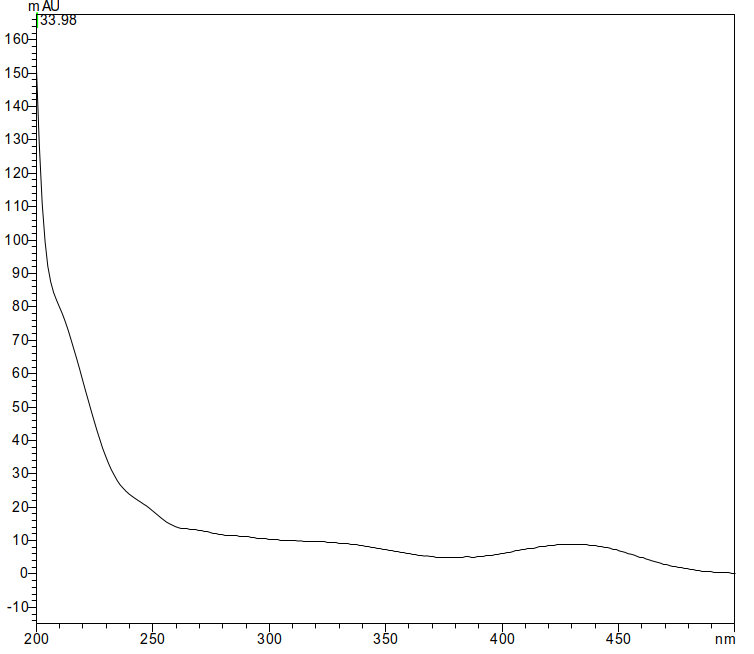
\includegraphics[width=\textwidth]{figures/Kapitel6/Reaktion3h/YCC3398.png}
    \caption{}
    \label{fig:YCC3398}
  \end{subfigure}
  \hfill
  \begin{subfigure}[b]{0.5\textwidth}
    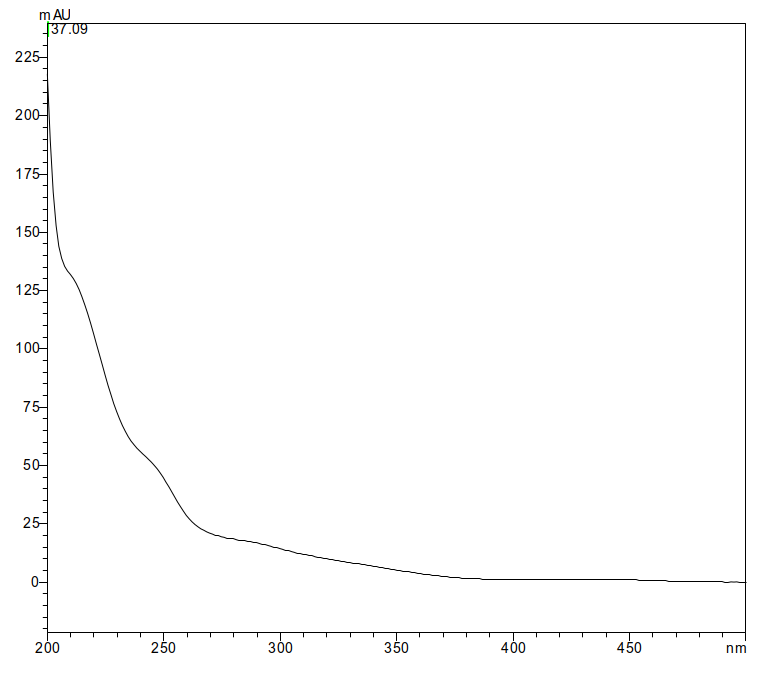
\includegraphics[width=\textwidth]{figures/Kapitel6/Reaktion3h/DNCC3709.png}
    \caption{}
    \label{fig:DNCC3709}
  \end{subfigure}
  
  \begin{subfigure}[b]{0.5\textwidth}
    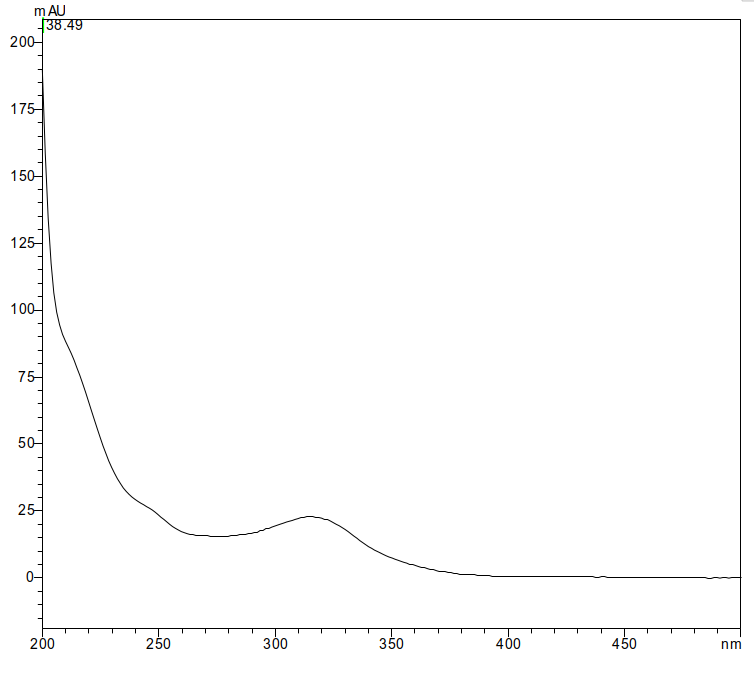
\includegraphics[width=\textwidth]{figures/Kapitel6/Reaktion3h/NCC3849.png}
    \caption{}
    \label{fig:NCC3849}
  \end{subfigure}
  \hfill
  \begin{subfigure}[b]{0.5\textwidth}
    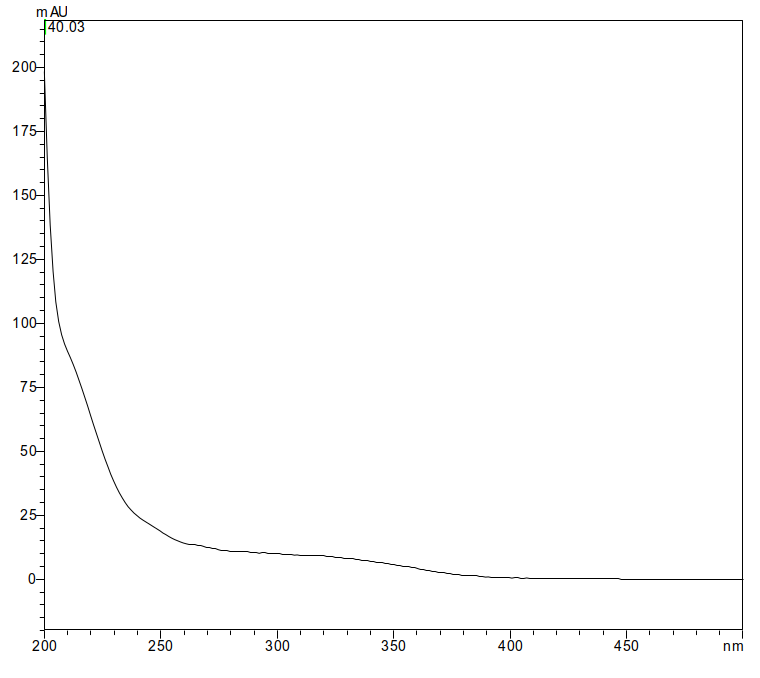
\includegraphics[width=\textwidth]{figures/Kapitel6/Reaktion3h/DNCC4003.png}
    \caption{}
    \label{fig:DNCC4003}
  \end{subfigure}
  
  \begin{subfigure}[b]{0.5\textwidth}
    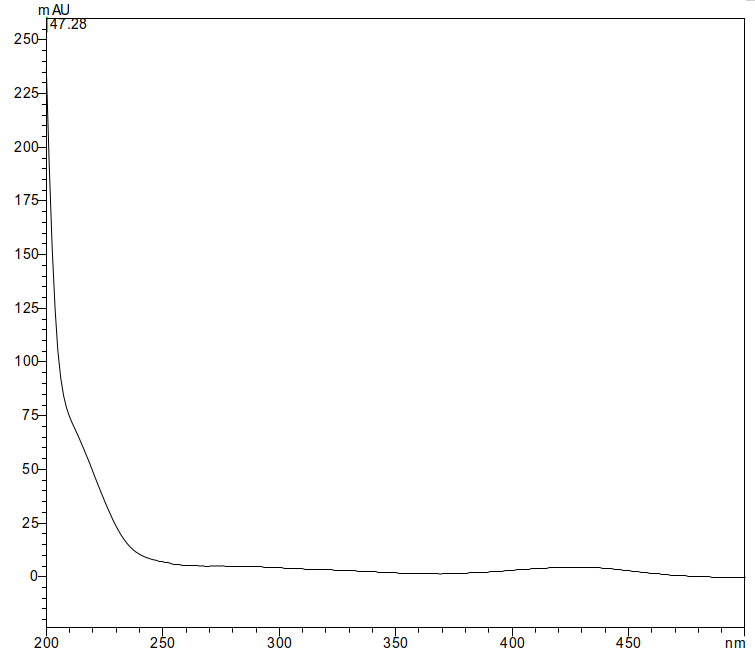
\includegraphics[width=\textwidth]{figures/Kapitel6/Reaktion3h/YCC4728.png}
    \caption{}
    \label{fig:YCC4728}
  \end{subfigure}
  \caption[UV/Vis online Spektren mit der Charakteristik eines YCC bei 33.98min., eines DNCC bei 37.09min. eines NCC bei 38.94min., eines DNCC bei 40.03min. sowie eines YCC bei 47.28min., Quelle: Author]{UV/Vis online Spektren: charakeristisch für (a) \gls{YCC} - RT = 33.98min., (b) \gls{DNCC} - RT = 37.09min., (c) \gls{NCC} - RT = 38.94min., (d) \gls{DNCC} - RT = 40.03min., (e) \gls{YCC} - RT = 47.28min.}
\end{figure}



\chapter{Strukturaufklärung der Chl-Kataboliten mit ESI-MS}

\section{Identifizierte Chl-Kataboliten}

\subsection{Bo-DYCC}

\begin{figure}[!htbp]
  \centering
  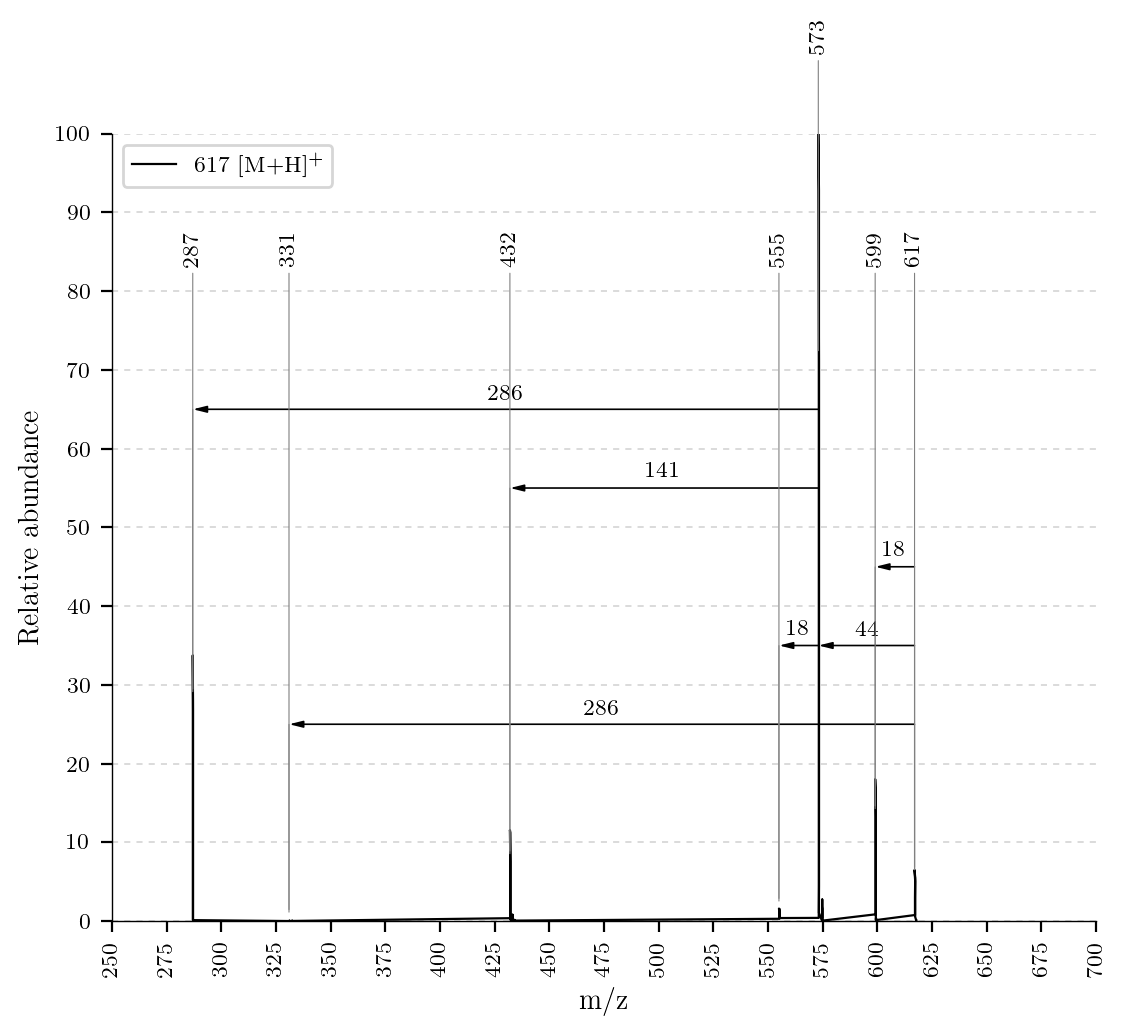
\includegraphics[width=\textwidth, height=0.7\textwidth]{figures/Kapitel7/Kataboliten/VWA_MS_617.png}
  \caption[LC-MS Chromatogramm vor der Reaktion, Quelle: Author]{\gls{lcms} Chromatogramm}
  \label{fig:LCMSChromatogramm}
\end{figure}

\begin{figure}[!htbp]
  \centering
  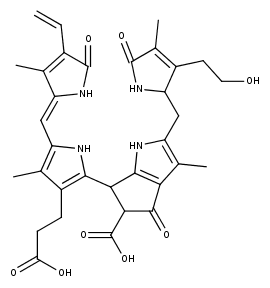
\includegraphics[scale=0.6]{figures/Kapitel7/Kataboliten/fragmentation_structures/VWA_Katabolit_617.png}
  \caption[LC-MS Chromatogramm vor der Reaktion, Quelle: Author]{\gls{lcms} Chromatogramm}
  \label{fig:LCMSChromatogramm}
\end{figure}

\begin{figure}[!htbp]
  \begin{subfigure}[b]{0.5\textwidth}
    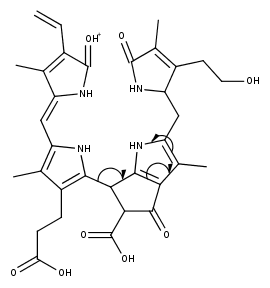
\includegraphics[width=\textwidth]{figures/Kapitel7/Kataboliten/fragmentation_structures/VWA_Katabolit_617_MH_RingD-RingC_331_electronMovement.png}
    \caption{}
    \label{fig:NCC2725}
  \end{subfigure}
  \hfill
  \begin{subfigure}[b]{0.5\textwidth}
    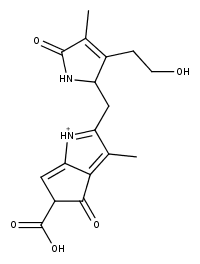
\includegraphics[width=\textwidth]{figures/Kapitel7/Kataboliten/fragmentation_structures/VWA_Katabolit_617-RingD-RingC_331.png}
    \caption{}
    \label{fig:DNCC2991}
  \end{subfigure}
  \caption[Online-UV/Vis Spektren mit der Charakteristik eines NCC bei 27.10min., eines DNCC bei 29.75min. sowie eines YCC bei 30.94min., Quelle: Autor]{Online-UV/Vis Spektren: (a) charakteristisch für einen \gls{NCC} - RT = 27.25min., (b) charakteristisch für einen \gls{DNCC} - RT = 29.91min., (c) charakteristisch für einen \gls{YCC} - RT = 30.94min.}
\end{figure}

\subsection{Bo-DNCC}

\begin{figure}[!htbp]
  \centering
  \includegraphics[width=\textwidth, height=0.7\textwidth]{figures/Kapitel7/Kataboliten/VWA_MS_619.png}
  \caption[LC-MS Chromatogramm vor der Reaktion, Quelle: Author]{\gls{lcms} Chromatogramm}
  \label{fig:LCMSChromatogramm}
\end{figure}

\begin{figure}[!htbp]
  \begin{subfigure}[b]{0.5\textwidth}
    \includegraphics[width=\textwidth]{figures/Kapitel7/Kataboliten/fragmentation_structures/VWA_Katabolit_619_MH-CO2-RingA-RIngD_311_electronMovement.png}
    \caption{}
    \label{fig:NCC2725}
  \end{subfigure}
  \hfill
  \begin{subfigure}[b]{0.5\textwidth}
    \includegraphics[width=\textwidth]{figures/Kapitel7/Kataboliten/fragmentation_structures/VWA_Katabolit_619-CO2-RingA-RingD_311.png}
    \caption{}
    \label{fig:DNCC2991}
  \end{subfigure}
  \caption[Online-UV/Vis Spektren mit der Charakteristik eines NCC bei 27.10min., eines DNCC bei 29.75min. sowie eines YCC bei 30.94min., Quelle: Autor]{Online-UV/Vis Spektren: (a) charakteristisch für einen \gls{NCC} - RT = 27.25min., (b) charakteristisch für einen \gls{DNCC} - RT = 29.91min., (c) charakteristisch für einen \gls{YCC} - RT = 30.94min.}
\end{figure}

\begin{figure}[!htbp]
  \begin{subfigure}[b]{0.5\textwidth}
    \includegraphics[width=\textwidth]{figures/Kapitel7/Kataboliten/fragmentation_structures/VWA_Katabolit_619-CO2-RingD-RingA_311_Mesomer1.png}
    \caption{}
    \label{fig:NCC2725}
  \end{subfigure}
  \hfill
  \begin{subfigure}[b]{0.5\textwidth}
    \includegraphics[width=\textwidth]{figures/Kapitel7/Kataboliten/fragmentation_structures/VWA_Katabolit_619-CO2-RingD-RingA_311_Mesomer2.png}
    \caption{}
    \label{fig:DNCC2991}
  \end{subfigure}
  \caption[Online-UV/Vis Spektren mit der Charakteristik eines NCC bei 27.10min., eines DNCC bei 29.75min. sowie eines YCC bei 30.94min., Quelle: Autor]{Online-UV/Vis Spektren: (a) charakteristisch für einen \gls{NCC} - RT = 27.25min., (b) charakteristisch für einen \gls{DNCC} - RT = 29.91min., (c) charakteristisch für einen \gls{YCC} - RT = 30.94min.}
\end{figure}

\subsection{Bo-YCC}

\begin{figure}[!htbp]
  \centering
  \includegraphics[width=\textwidth, height=0.7\textwidth]{figures/Kapitel7/Kataboliten/VWA_MS_645-1.png}
  \caption[LC-MS Chromatogramm vor der Reaktion, Quelle: Author]{\gls{lcms} Chromatogramm}
  \label{fig:LCMSChromatogramm}
\end{figure}

\begin{figure}[!htbp]
  \centering
  \includegraphics[scale=0.6]{figures/Kapitel7/Kataboliten/fragmentation_structures/VWA_Katabolit_645_vorReaktion.png}
  \caption[LC-MS Chromatogramm vor der Reaktion, Quelle: Author]{\gls{lcms} Chromatogramm}
  \label{fig:LCMSChromatogramm}
\end{figure}

\subsection{Bo-NCC-3}

\begin{figure}[!htbp]
  \centering
  \includegraphics[width=\textwidth, height=0.7\textwidth]{figures/Kapitel7/Kataboliten/VWA_MS_647.png}
  \caption[LC-MS Chromatogramm vor der Reaktion, Quelle: Author]{\gls{lcms} Chromatogramm}
  \label{fig:LCMSChromatogramm}
\end{figure}

\begin{figure}[!htbp]
  \begin{subfigure}[b]{0.5\textwidth}
    \includegraphics[width=\textwidth]{figures/Kapitel7/Kataboliten/fragmentation_structures/VWA_Katabolit_647.png}
    \caption{}
    \label{fig:NCC2725}
  \end{subfigure}
  \hfill
  \begin{subfigure}[b]{0.5\textwidth}
    \includegraphics[width=\textwidth]{figures/Kapitel7/Kataboliten/fragmentation_structures/VWA_Katabolit_647-CO2-RingD_480_MH_electronMovement.png}
    \caption{}
    \label{fig:DNCC2991}
  \end{subfigure}
  \caption[Online-UV/Vis Spektren mit der Charakteristik eines NCC bei 27.10min., eines DNCC bei 29.75min. sowie eines YCC bei 30.94min., Quelle: Autor]{Online-UV/Vis Spektren: (a) charakteristisch für einen \gls{NCC} - RT = 27.25min., (b) charakteristisch für einen \gls{DNCC} - RT = 29.91min., (c) charakteristisch für einen \gls{YCC} - RT = 30.94min.}
\end{figure}

\begin{figure}[!htbp]
  \begin{subfigure}[b]{0.5\textwidth}
    \includegraphics[width=\textwidth]{figures/Kapitel7/Kataboliten/fragmentation_structures/VWA_Katabolit_647-CO2-RingD_480_MH_Enolform.png}
    \caption{}
    \label{fig:NCC2725}
  \end{subfigure}
  \hfill
  \begin{subfigure}[b]{0.5\textwidth}
    \includegraphics[width=\textwidth]{figures/Kapitel7/Kataboliten/fragmentation_structures/VWA_Katabolit_647-CO2-RingD_480_MH_Ketoform.png}
    \caption{}
    \label{fig:DNCC2991}
  \end{subfigure}
  \caption[Online-UV/Vis Spektren mit der Charakteristik eines NCC bei 27.10min., eines DNCC bei 29.75min. sowie eines YCC bei 30.94min., Quelle: Autor]{Online-UV/Vis Spektren: (a) charakteristisch für einen \gls{NCC} - RT = 27.25min., (b) charakteristisch für einen \gls{DNCC} - RT = 29.91min., (c) charakteristisch für einen \gls{YCC} - RT = 30.94min.}
\end{figure}

\subsection{Bo-NCC-1}

\begin{figure}[!htbp]
  \centering
  \includegraphics[width=\textwidth, height=0.7\textwidth]{figures/Kapitel7/Kataboliten/VWA_MS_793.png}
  \caption[LC-MS Chromatogramm vor der Reaktion, Quelle: Author]{\gls{lcms} Chromatogramm}
  \label{fig:LCMSChromatogramm}
\end{figure}



\section{Reaktionsprodukte der Chl-Kataboliten}

\subsection{Reaktionsprodukt von Bo-DYCC}

\begin{figure}[!htbp]
  \centering
  \includegraphics[width=\textwidth, height=0.7\textwidth]{figures/Kapitel7/Kataboliten/VWA_MS_631.png}
  \caption[LC-MS Chromatogramm vor der Reaktion, Quelle: Author]{\gls{lcms} Chromatogramm}
  \label{fig:LCMSChromatogramm}
\end{figure}

\begin{figure}[!htbp]
  \centering
  \includegraphics[width=\textwidth, height=0.7\textwidth]{figures/Kapitel7/Kataboliten/VWA_MS_645-2.png}
  \caption[LC-MS Chromatogramm vor der Reaktion, Quelle: Author]{\gls{lcms} Chromatogramm}
  \label{fig:LCMSChromatogramm}
\end{figure}


\begin{figure}[!htbp]
  \begin{subfigure}[b]{0.5\textwidth}
    \includegraphics[width=\textwidth]{figures/Kapitel7/Kataboliten/fragmentation_structures/VWA_Katabolit_631.png}
    \caption{}
    \label{fig:NCC2725}
  \end{subfigure}
  \hfill
  \begin{subfigure}[b]{0.5\textwidth}
    \includegraphics[width=\textwidth]{figures/Kapitel7/Kataboliten/fragmentation_structures/VWA_Katabolit_645_nachReaktion.png}
    \caption{}
    \label{fig:DNCC2991}
  \end{subfigure}
  \caption[Online-UV/Vis Spektren mit der Charakteristik eines NCC bei 27.10min., eines DNCC bei 29.75min. sowie eines YCC bei 30.94min., Quelle: Autor]{Online-UV/Vis Spektren: (a) charakteristisch für einen \gls{NCC} - RT = 27.25min., (b) charakteristisch für einen \gls{DNCC} - RT = 29.91min., (c) charakteristisch für einen \gls{YCC} - RT = 30.94min.}
\end{figure}

\subsection{Reaktionsprodukt von Bo-DNCC}

\begin{figure}[!htbp]
  \centering
  \includegraphics[width=\textwidth, height=0.7\textwidth]{figures/Kapitel7/Kataboliten/VWA_MS_633.png}
  \caption[LC-MS Chromatogramm vor der Reaktion, Quelle: Author]{\gls{lcms} Chromatogramm}
  \label{fig:LCMSChromatogramm}
\end{figure}

\begin{figure}[!htbp]
  \centering
  \includegraphics[scale=0.6]{figures/Kapitel7/Kataboliten/fragmentation_structures/VWA_Katabolit_633.png}
  \caption[LC-MS Chromatogramm vor der Reaktion, Quelle: Author]{\gls{lcms} Chromatogramm}
  \label{fig:LCMSChromatogramm}
\end{figure}

\subsection{Reaktionsprodukt von Bo-YCC}

Wurde nicht gefunden.

\subsection{Reaktionsprodukt von Bo-NCC-3}

\begin{figure}[!htbp]
  \centering
  \includegraphics[width=\textwidth, height=0.7\textwidth]{figures/Kapitel7/Kataboliten/VWA_MS_661.png}
  \caption[LC-MS Chromatogramm vor der Reaktion, Quelle: Author]{\gls{lcms} Chromatogramm}
  \label{fig:LCMSChromatogramm}
\end{figure}

\subsection{Reaktionsprodukt von Bo-NCC-1}

Wurde nicht gefunden.


\addpart{Zusammenfassung und Fazit}

\chapter{Ergebnisse}

Da die Ergebnisse bereits im experimentellen Teil ausführlich behandelt worden sind, folgt hier nur eine Übersicht über die identifizierten Chl-Kataboliten.

\section{Auflistung aller identifizierten Chl-Kataboliten und deren Reaktionsprodukte}

In Tabelle \ref{tab:LCMSKatabolitenRPListe} werden alle Verbindungen aufgelistet, die ich im Rahmen meiner Arbeit in den diversen Experimenten identifizieren konnte. Index zur Tabelle:

\begin{description}[align=right,labelwidth=3cm]
  \item [Chl-Katabolit] . . . vorgeschlagene Bezeichnung für mit großer Sicherheit identifizierte Chl-Kataboliten
  \item [Summenformel] . . . die Summenformel des [M+H]\textsuperscript{+} Ions, gemessen in ESI-MS und LC-MS Experimenten - bei mit * gekennzeichneten handelt es sich um die Summenformel des ungeladenen Chl-Kataboliten.
  \item [M+H] . . . Molekülmasse des [M+H]\textsuperscript{+} Ions, die in ESI-MS oder LC-MS Experimente gemessen wurde
  \item [Frag. I] . . . gibt an, ob bei den ESI-MS Experimenten ein Fragmentierungsdiagramm erstellt wurde
  \item [MS-Leafspray] . . . Molekülmasse des [M+K]\textsuperscript{+} Ions, sofern mit MS-Leafspray gemessen
  \item [Frag. II] . . . gibt an, ob bei den MS-Leafspray Experimenten ein Fragmentierungsdiagramm erstellt wurde
  \item [Typ] . . . gibt die Art des Chl-Kataboliten an, sofern dies klar ist - bei mit * gekennzeichneten handelt es sich um Anhydride
  \item [HPLC] . . . gibt an, ob Chl-Katabolit mithilfe von UV/Vis Spektren in der HPLC identifiziert werden konnte
  \item [H.] . . . (Herkunft) gibt an, ob es sich bei der Verbindung um ein Reaktionsprodukt handelt und wenn ja, welcher Chl-Katabolit das Edukt war
\end{description} 


\begin{sidewaystable*}[!htbp]\centering
  \ra{1.3}
  
  \begin{tabular}{ccccccccc}\toprule
 Chl-Katabolit & Summenformel & [M+H]\textsuperscript{+} & Frag. I & MS-Leafspray & Frag. II & Typ & HPLC & H. \\
\midrule
\rowcolor{black!20} Bo-DYCC & \ch{C33H37O8N4} & 617.2599 & \checkmark & x & x & DYCC & 30.94? & -\\
 Bo-DNCC & \ch{C33H39O8N4} & 619.2798 & \checkmark & 657 & \checkmark & DNCC & 26.72 & -\\ 
\rowcolor{black!20} • & \ch{C34H37O8N4} & 629.2641 & x & x & x & • & - & -\\ 
 - & \ch{C34H39O8N4} & 631.2795 & \checkmark & x & x & DYCC & 29.91, 30.94 & Bo-DYCC\\ 
\rowcolor{black!20} - & \ch{C34H41O8N4} & 633.2955 & \checkmark & x & x & DNCC & 28.8 & Bo-DNCC\\ 
 • & \ch{C36H33O7N4} & 633.2339 & x & x & x & • & - & -\\ 
\rowcolor{black!20} Bo-YCC & \ch{C34H37O9N4} & 645.2593 & \checkmark & x & x & YCC & - & -\\ 
 - & \ch{C35H41O8N4} & 645.2953 & x & x & x & DYCC & - & Bo-DYCC\\ 
\rowcolor{black!20} Bo-NCC-3 & \ch{C34H39O9N4} & 647.2748 & \checkmark & 685 & \checkmark & NCC & 33.04 & -\\ 
 • & \ch{C34H35O10N4} & 659.2348 & x & x & x & • & - & -\\
\rowcolor{black!20} - & \ch{C35H39O9N4} & 659.2741 & \checkmark & x & x & YCC & 37.09 & Bo-YCC\\
 - & \ch{C35H41O9N4} & 661.2902 & \checkmark & x & x & NCC & - & Bo-NCC-3\\
\rowcolor{black!20} - & \ch{C36H43O9N4} & 675.306 & \checkmark & x & x & NCC & - & Bo-NCC-3\\
 Bo-DNCC-2 & \ch{C39H47O13N4} & 779.3181 & x & x & x & DNCC & - & -\\ 
\rowcolor{black!20} Bo-NCC-1 & \ch{C40H49O13N4} & 793.3336 & \checkmark & 831 & \checkmark & NCC & 29.91 & -\\ 
 - & \ch{C40H51O13N4} & 795.3491 & \checkmark & x & x & - & - & -\\ 
\rowcolor{black!20} - & \ch{C41H51O13N4} & 807.3491 & \checkmark & x & x & NCC & 40.03 & Bo-NCC-1\\ 
 - & \ch{C41H53O13N4} & 809.3649 & x & x & x & - & - & 795\\ 
\rowcolor{black!20} - & \ch{C42H53O13N4} & 821.3652 & x & x & x & NCC & 47.28 & Bo-NCC-1\\ 
 - & \ch{C35H41N4O9}* & x & x & 699 & \checkmark & DNCC* & - & Bo-DNCC \\ 
\rowcolor{black!20} - & \ch{C36H40N4O10}* & x & x & 727 & \checkmark & NCC* & & Bo-NCC-3\\ 
 - & \ch{C42H50N4O14}* & x & x & 873 & \checkmark & NCC* & - & Bo-NCC-1 \\ 
\bottomrule
  \end{tabular}
  
  \caption[Übersicht über die Chl-Kataboliten des Brokkoliblattes unter Berücksichtigun der Erkenntnisse aller Methoden, Quelle: Autor]{Übersicht über die gefundenen Chl-Kataboliten des Brokkoliblattes und ihren Reaktionsprodukten}
  \label{tab:LCMSKatabolitenRPListe}
\end{sidewaystable*}

\chapter{Diskussion}

Im Folgenden werden die im Experimentellen Teil beschriebenen Ergebnisse in Hinblick auf die in Kapitel \ref{sec:Themenstellung} gestellten Fragen analysiert. Es werden dabei nur die wichtigsten, sogenannte Highlights herausgenommen, da eine genauere Ausführung den Rahmen sprengen würde.

\section{zur direkten Analyse, MS Leafspray und der Reaktion mit Essigsäureanhydrid}

Wie in Kapitel \ref{sec:MSLeafspray} ersichtlich, konnten die \gls{Chl-K}en erfolgreich in einer direkten Analyse mithilfe von MS Leafspray identifiziert werden.  

Zu Beginn waren die Experimente jedoch von deutlichen Misserfolgen geprägt. Es scheiterte z.B. bereits daran, ein schönes, konstantes Signal im Massenspektrometer zu bekommen. Auch ein Optimieren des Signals durch Kalibrierung und andere Methoden brachte keine Besserung. Erst die Entwicklung der in Kapitel \ref{sec:MSLeafspray} beschriebenen Blattvorbereitungstechnik(en) konnte zusammen mit der Erkenntnis, dass man gelegentlich vom positiven in den negativen Ionenmodus schalten muss zu schönen und vor allem verwertbaren Massenspektren und Fragmentierungsdiagrammen führen\footnote{diese Erkenntnis ist einem Zufall zu verdanken: während dem Messen verschwand das Signal plötzlich und ich befürchtete schon, das Massenspektrometer verstopft zu haben (eine Katastrophe) - nach einem mehr oder weniger zufälligem Umschalten in den negativen Ionenmodus und dem sofortigen Zurückschalten in den positiven war das Signal wieder in vollster Intensität vorhanden}. 

Nachdem die \gls{Chl-K}en des Brokkoliblattes erfolgreich identifiziert wurden, konnten mit der gleichen Methode auch die Reaktionsprodukte der \gls{Chl-K}en mit Essigsäureanhydrid gemessen werden. Unter Verwendung von Essigsäureanhydrid als LM konnten dabei sogar die Anhydride als Reaktionsprodukte identifiziert werden.

Zur Reaktivität der Carbonsäuren wurde beobachtet, dass die freie Carbonsäure an Position 8\textsuperscript{2} deutlich reaktiver ist wie jene an Position 12\textsuperscript{2}. Vermutlich ist dies durch die bevorzugte sterische Umgebung begründet, wobei dies bisher reine Spekulation ist.

\section{zu den Fragmentierungsdiagrammen und Strukturaufklärung}

Es konnten für alle mit MS Leafspray gemessenen Verbindungen Fragmentierungsdiagramme erfolgreich aufgenommen werden. In der Arbeit wurde vorgeschlagen, dass eine Analyse dieser über den Vergleich von Minima und Maxima möglich ist. Auf diese Weise kann ein Einblick auf massenspektrometrische Eigenschaften der Verbindungen gewonnen werden. 

Es wird vermutet, dass die Fragmentierungsdiagramme charakteristisch für einen Chl-Kataboliten sind, weil diesselben Diagramme bei zu unterschiedlichen Zeitpunkten durchgeführten Experimenten erstellt wurden. Es handelt sich dabei jedoch nur um eine Theorie, die noch in weiterer, gezielter experimenteller Arbeit verifiziert werden müsste.

Um einen Blick in die Zukunft zu wagen, könnte man diese Fragmentierungsdiagramme verwenden, um eine Schnellidentifikation von Chl-Kataboliten durchzuführen. Ein Anwendungsgebiet wäre hier beispielsweise die Landwirtschaft, in der ein Bauer mithilfe von MS Leafspray \textit{am Feld} Chl-Kataboliten identifizieren könnte. Um diese Schnellidentifikation zu programmieren, könnte man auf die Methode des Deep-Learnings zurückgreifen, die ein Analysieren der Diagramme erleichtern und vor allem automatisieren könnte. 

Unter Verwendung eines solchen Deep-Learning Netwerkes ist es außerdem denkbar, dass man aus den Fragmentierungsdiagramm weitere Strukturmerkmale \textit{herauskitzeln} kann, was einen Fortschritt in Bezug auf Strukturaufklärung mit dem Massenspektrometer bedeuten würde.

Außerdem ist denkbar, dass über eine intensivere Erforschung der Fragmentierungsdiagramme ein tieferer Einblick in die Eigenschaften der chemischen Bindung in komplexen Molekülen gewonnen werden kann. Auch hier ist eine Anwendung von DeepLearning denkbar.\\

Im Folgenden wird eine Theorie zur Interpretation der im CID-Modus aufgenommenen Fragmentierungsdiagramme entwickelt. Im Massenspektrometer kommt es durch teilweise Umwandlung kinetischer Energie in intramolekulare Energie zur  Anregung des Molekül und dementsprechend zu Schwingungen desselben. Diese Schwingungen führen letztendlich zum Bindungsbruch und zu den messbaren Fragmenten. Bei der Erstellung der Fragmentierungsdiagramme wurde die Intensität dieser Fragmente zur aufgewendeten \gls{nKE} gemessen. \\

Was bei der Betrachtung der Diagramme auffällt, ist, dass sie Minima und Maxima besitzen, die im Praktischen Teil der Arbeit ausführlich beschrieben worden sind. Außerdem nehmen die Intensitäten bei höheren Energien zumeist ab. Die meisten Maxima befinden sich in einem Bereich von 10 bis 50 \gls{nKE}. 

\gls{Chl-K}en sind von ihrer räumlichen Struktur komplexe Moleküle und können aufgrund von Drehungen um Einfachbindungen diverse räumliche Strukturen annehmen, die aufgrund von sterischen Effekten thermodynamisch nicht gleich stabil sind. Wenn ein solcher \gls{Chl-K} energetisch angeregt wird und demnach schwingt, gibt es vermutlich bestimmte energetisch stabile räumliche Anordnungen, die abhängig von der \gls{nKE} sind. Das könnte bedeuten, dass es bestimmte \gls{nKE}s gibt, die den \gls{Chl-K}en in bestimmte räumliche Anordnungen bringen, bei denen eine Abspaltung eines Ringes beispielsweise energetisch günstig ist. 

Nach diesem Modell wäre bei einer großen \gls{nKE} die Anregung so groß, dass es zu sterischen intramolekularen Hinderungen kommt, die Abspaltungen entweder gänzlich verhindern oder das Molekül zum unkontrollierten Auseinanderbrechen bringt. Das Entstehen von Maxima einer Abspaltung kann durch das Einnehmen eines für diese Abspaltung energetisch günstigen Zustandes erklärt werden. Minima könnten das Einnehmen eines Übergangszustandes beschreiben.

Bei der vorliegenden Betrachtung werden die Intensitäten der Abspaltungen aufgrund der unterschiedlichen Ionisierbarkeit nicht berücksichtigt. Es wird angenommen, dass die Ionisierbarkeit nicht von der \gls{nKE} abhängt.


\section{zum Vergleich direkte Analyse - klassischer Ansatz}

In Tabelle \ref{tab:ComparisonDirectClassic} werden die wesentlichen Unterschiede der beiden Analysemethoden, die ich während meiner Arbeit beobachten konnte, herausgearbeitet. Die Liste stellt nicht den Anspruch, vollständig zu sein.

\newcolumntype{C}[1]{>{\centering\arraybackslash}p{#1}}

\begin{table*}[!htbp]\centering
  \ra{1.3}
  
  \begin{tabular}{C{1cm}C{6cm}C{1cm}C{6cm}}\toprule
 +/- & direkte Analyse & +/- & klassischer Ansatz \\
\midrule
\rowcolor{black!20} + & kurze Blattvorbereitungszeit für die Analyse & - & lange Blattvorbereitungszeit für die Analyse (Aufreibung, Abzentrifugieren, ...) \\
 + & lange Analysezeiten, die z.B. für die Erstellung von Fragmentierungsdiagrammen verwendet werden kann & - & 75 min. Zeit vergeht, bis analysiert werden kann - erzeugen von Fragmentierungsdiagrammen nur über Sammeln in EPPIs möglich \\ 
\rowcolor{black!20} + & erlaubt einfache Isolierung von Anhydriden durch Verwendung von Acetonitril als LM & - & Isolierung von Anhydriden als Reaktionsprodukt schwer möglich, da bevorzugtes LM MeOH \\
 + & erlaubt Analyse von vielen Blättern in kurzer Zeit (ca. 30 min. pro Blatt, wenn man viele Chl-Kataboliten analysiert) & - & (fast) vollständige Analyse eines Blattes dauert bis zu 100 min., sofern sehr effizient gearbeitet wird \\ 
\rowcolor{black!20} - & man bekommt kein Chromatogramm, über das man alle Chl-Kataboliten potentiell herausfinden kann - es besteht die Gefahr, dass einige Chl-Kataboliten nicht analysiert werden & + & höhere Wahrscheinlichkeit des Auffindens von Chl-Kataboliten \\
 - & bevorzugt [M+K]\textsuperscript{+} Ionen & - & bevorzugt [M+H]\textsuperscript{+} Ionen \\ 
\rowcolor{black!20} - & Molekülmasse nur auf 1 signifikante Kommastelle messbar - Summenformel kann nicht berechnet werden & + & Molekülmasse auf 3 signifikante Kommastellen messbar - Möglichkeit, Summenformel zu berechnen \\
 + & theoretisch relativ einfach automatisierbar & - & aufwändig zu automatisieren \\ 
 \rowcolor{black!20} - & Massenspektrometer kann mit der Zeit verschmutzen & + & Massenspektrometer nicht so anfällig für ein Verschmutzen \\
\bottomrule
  \end{tabular}
  
  \caption[Vergleich beider Methoden, Quelle: Autor]{Vergleich von direkter Analyse mit einer klassischen Analyse}
  \label{tab:ComparisonDirectClassic}
\end{table*}

\pagebreak
\section{zum Vergleich Brokkoliblatt - Brokkolifrucht}

In meiner Arbeit wurden die Chl-Kataboliten des Brokkoliblattes untersucht. Im Vergleich zu einer kürzlich veröffentlichten Publikation \cite{ChlorophyllCatabolitesBroccoli}, in der die Brokkolifrucht analysiert wurde, konnte ich etwas mehr davon finden. Tabelle \ref{tab:ComparisonChlKatabolites} listet die jeweiligen Chl-Kataboliten auf:

\begin{table*}[!htbp]\centering
  \ra{1.3}
  
  \begin{tabular}{ccccccccc}\toprule
 Brokkoliblatt & Brokkolifrucht \\
\midrule
\rowcolor{black!20} Bo-NCC-1 & \checkmark \\
 x & Bo-NCC-2 \\ 
\rowcolor{black!20} Bo-NCC-3 & x \\
 Bo-DNCC & \checkmark \\ 
\rowcolor{black!20} Bo-DYCC & x \\
 Bo-YCC & x \\ 
\rowcolor{black!20} Bo-DNCC-2 & x \\
\bottomrule
  \end{tabular}
  
  \caption[Vergleich der Chl-Kataboliten - Brokkoliblatt und Brokkolifrucht, Quelle: Autor]{Vergleich der Chl-Kataboliten im Brokkoliblatt und der Brokkolifrucht}
  \label{tab:ComparisonChlKatabolites}
\end{table*}

\section{Rück- und Ausblick}

Ich denke, mir ist es gelungen, die in der Themenstellung gestellten Fragen weitestgehend zu beantworten. Was mich besonders freut, ist, dass ich mit MS Leafspray eine Methode verwenden sowie weiterentwickeln konnte, die meines Erachtens zusammen mit den Fragmentierungsdiagrammen ein enormes Zukunftspotential hat. Natürlich sind meine Erkenntnisse auf dem Gebiet der Fragmentierungsdiagramme noch nicht gefestigt, doch denke ich, dass ich mit dieser Arbeit einen wesentlichen Grundstein für weitere Forschung in diesem Gebiet legen konnte. 

Durch die parallele Analyse mit LC-MS konnte ein erfolgreicher Vergleich der beiden Methoden gemacht werden, was aufgrund der Bewährtheit von LC-MS ein gutes Licht auf MS Leafspray wirft.

Außerdem konnten andere Chl-Kataboliten im Brokkoliblatt nachgewiesen werden wie in der Frucht an sich, was neue Fragen zum Verständnis des Chl-Abbauprozesses aufwirft.

Demnach leiste ich mit dieser Arbeit einen wesentlichen Beitrag zur Methodenverbesserung, Analyseerweiterung und dem Verständnis des Abbauweges des Chlorophylls im Allgemeinen. Für mich persönlich gilt, dass ich durch diese Arbeit meine Persönlichkeit wesentlich weiterentwickeln konnte, insbesondere was eigenständiges Arbeiten in jeglicher Hinsicht und Sammeln von Erfahrung anbelangt. 

%Ich möchte betonen, dass die Erstellung dieser VWA einiges an Arbeit und vor allem Zeit beanspruchte. Zum Einen war es während meinem einmonatigem Praktikum schwer, sich auf einige wenige Sachen zu konzentrieren, um sinnvoll verwertbare Ergebnisse zu bekommen. Außerdem war das Planen der täglichen Experimente eine Herausforderung für sich. Doch mit der Zeit konnte ich mich in meiner Arbeitsweise zunehmend verbessern und erreichte somit eine große Effizienz\footnote{zu Bestzeiten gelangen mir 4 HPLC Läufe an einem Arbeitstag - das entsprich 5h}. In dem mir zur Verfügung stehendem, kurzem Zeitraum von 1 Monat war es nicht immer leicht, einen Mittelweg zwischen Analyse der Ergebnisse und Durchführen von Experimenten zu finden. Das Resultat war, dass der Großteil der Datenauswertung nach meinem Praktikum erfolgte.

%%----------------------------------------------------------------
%
%  File    :  thesis-style.tex
%
%  Author  :  Keith Andrews, IICM, TU Graz, Austria
% 
%  Created :  27 May 93
% 
%  Changed :  19 Feb 2004
% 
% styling and technical implementation adopted 2011 by Karl Voit
%----------------------------------------------------------------

%% defined an anvironment for the style Keith used to use:
\newenvironment{mykeithtabbing}[1]{%%
\begin{tabular}{lp{0.9\hsize}}
}{%%
\end{tabular}
}

\newcommand{\mybadgood}[2]{%%
\begin{mykeithtabbing}
{}\emph{Bad:}  & \sout{#1}  \\
\emph{Good:}   & #2  \\
\end{mykeithtabbing}

}

\chapter{Language and Writing Style}
\label{chap:Style}

\begin{framed}

  This chapter is an adopted version of a single chapter of
  \citeauthor{KeithThesis} thesis template \cite{KeithThesis} in its
  version from 2011-12-11.

  The reason why \cite{KeithThesis} is not recommended to be used instead
  of this template is its more \enquote{traditional} \LaTeX{}
  implementation. But the information contained regarding \enquote{How
    to write a thesis} is generally brilliant and worth reading.

  Using this chapter here is meant as a teaser. If you do like this
  chapter, please go and download the full template to read its
  content:~\cite{KeithThesis}.

  What was modified from the original chapter:
    \begin{itemize}
    \item strikethrough of bad examples
    \item minor typographical details
    \item technical modifications
      \begin{itemize}
      \item moved citations from \verb+\citet{}+ and
        \verb+\citep{}+ to \verb+\textcite{}+ and \verb+\cite{}+
      \item changed quoting style to \verb+\enquote{}+
      \item created various commands and environments to encapsulate
        format
      \end{itemize}
    \end{itemize}
\end{framed}

The classic reference for English writing style and grammar is
\textcite{StrunkWhite}. The original text is now available for free
online \cite{Strunk}, so there is no excuse at all for writing poor
English. Readers should consult it first, then continue reading this
chapter. Another good free guide is \textcite{NASAGuide}.

%orig% The classic reference for English writing style and grammar is
%orig% \citet{StrunkWhite}. The original text is now available for free
%orig% online \citep{Strunk}, so there is no excuse at all for writing poor
%orig% English. Readers should consult it first, then continue reading this
%orig% chapter. Another good free guide is \citet{NASAGuide}.


\textcite{Zobel-WritingCompSci} and \textcite{BugsInWriting} are guides
specifically aimed at computer science students.
\textcite{Phillips-HowGetPhD} gives practical advice for PhD
students.

The following Sections~\ref{sec:Clear} and \ref{sec:Gender} are
adapted from the CHI'94 language and writing style guidelines.







\section{Some Basic Rules of English}

There are a few basic rules of English for academic writing, which are
broken regularly by my students, particularly if they are non-native
speakers of English. Here are some classic and often encountered
examples:

\begin{itemize}

\item \emph{Never} use I, we, or you.

Write in the passive voice (third person).

\mybadgood{You can do this in two ways.}{There are two ways this can be done.}


\item \emph{Never} use he or she, his or her.

Write in the passive voice (third person).

\mybadgood{The user speaks his thoughts out loud.}{The thoughts of the user are spoken out loud.}


See Section~\ref{sec:Gender} for many more examples.



\item Stick to a consistent dialect of English. Choose either
  British or American English and keep to it throughout the
  whole of your thesis.



\item Do \emph{not} use slang abbreviations such as \enquote{it's},
  \enquote{doesn't}, or \enquote{don't}.

Write the words out in full: \enquote{it is}, \enquote{does not}, and \enquote{do not}.

\mybadgood{It's very simple to\ldots}{It is very simple to\ldots}




\item Do \emph{not} use abbreviations such as \enquote{e.\,g.} or
  \enquote{i.\,e.}. 

Write the words out in full: \enquote{for example} and \enquote{that is}.

\mybadgood{\ldots in a tree, e.\,g.\xspace{}the items\ldots}{\ldots in a tree, for example the items\ldots}



\item Do \emph{not} use slang such as \enquote{a lot of}.

\mybadgood{There are a lot of features\ldots}{There are many features\ldots}



\item Do \emph{not} use slang such as \enquote{OK} or \enquote{big}.

\mybadgood{\ldots are represented by big areas.}{\ldots are represented by large areas.}



\item Do \emph{not} use slang such as \enquote{gets} or \enquote{got}.

Use \enquote{becomes} or \enquote{obtains}, or use the passive voice (third
person).

\mybadgood{The radius gets increased\ldots}{The radius is increased\ldots}

\mybadgood{The user gets disoriented\ldots}{The user becomes disoriented\ldots}




\item \emph{Never} start a sentence with \enquote{But}.

Use \enquote{However,} or \enquote{Nevertheless,}. Or consider joining the
sentence to the previous sentence with a comma.

\mybadgood{But there are numerous possibilities\ldots}{However, there are numerous possibilities\ldots}



\item \emph{Never} start a sentence with \enquote{Because}.

Use \enquote{Since}, \enquote{Owing to}, or \enquote{Due to}. Or turn the two
halves of the sentence around.




\item \emph{Never} start a sentence with \enquote{Also}. Also should
be placed in the middle of the sentence.

\mybadgood{Also the target users are considered.}{The target users are also considered.}



\item Do \emph{not} use \enquote{that} as a connecting word.

Use \enquote{which}.

\mybadgood{\ldots a good solution that can be computed easily.}{\ldots a good solution which can be computed easily.}




\item Do \emph{not} write single-sentence paragraphs. 

Avoid writing two-sentence paragraphs. A paragraph should contain at
least three, if not more, sentences.


\end{itemize}



% rules on the use of a comma in lists
% http://en.wikipedia.org/wiki/Serial_comma








\section{Avoid Austrianisms}
\label{sec:Austrianisms}


I see these mistakes time and time again. Please do not
let me read one of them in your work.



\begin{itemize}


\item \enquote{actual}~$\ne$~\enquote{current} 

If you mean \enquote{aktuell} in German, you probably mean
\enquote{current} in English.

\mybadgood{The actual selection is cancelled.}{The current selection is cancelled.}




\item \enquote{allows to} is not English.

\mybadgood{The prototype allows to arrange components\ldots}%%
{The prototype supports the arrangement of components\ldots}

% they allow to achieve



\item \enquote{enables to} is not English.

\mybadgood{it enables to recognise meanings\ldots}{it enables the recognition of meanings\ldots}



\item \enquote{according}~$\ne$~\enquote{corresponding} 

\mybadgood{For each browser, an according package is created.}{For each browser, a corresponding package is created.}



\item \enquote{per default} is not English.

Use \enquote{by default}.

\mybadgood{Per default, the cursor is red.}{By default, the cursor is red.}




\item \enquote{As opposed to} is not English.

Use \enquote{In contrast to}.

\mybadgood{As opposed to C, Java is object-oriented.}{In contrast to C, Java is object-oriented.}


\item \enquote{\emph{anything}-dimensional} is spelt with a hyphen.

For example: two-dimensional, three-dimensional.



\item \enquote{\emph{anything}-based} is spelt with a hyphen.

For example: tree-based, location-based.



\item \enquote{\emph{anything}-oriented} is spelt with a hyphen.

For example: object-oriented, display-oriented.


\item \enquote{\emph{anything}-side} is spelt with a hyphen.

For example: client-side, server-side.


\item \enquote{\emph{anything}-friendly} is spelt with a hyphen.

For example: user-friendly, customer-friendly.


\item \enquote{\emph{anything}-to-use} is spelt with hyphens.

For example: hard-to-use, easy-to-use.



\item \enquote{realtime} is spelt with a hyphen if used as
  an adjective, or as two separate words if used as a noun.

\mybadgood{\ldots using realtime shadow casting.}{\ldots using real-time shadow casting.}
\mybadgood{\ldots display the object in realtime.}{\ldots display the object in real time.}


\end{itemize}












\section{Clear Writing}
\label{sec:Clear}

The written and spoken language of your thesis is English as
appropriate for presentation to an international audience. Please take
special care to ensure that your work is adapted to such an audience.
In particular:

\begin{itemize}
\item Write in a straight-forward style, using simple sentence
  structure.

\item Use common and basic vocabulary. For example, use \enquote{unusual}
  for \enquote{arcane}, and \enquote{specialised} for \enquote{erudite}.

\item Briefly define or explain all technical vocabulary the first
  time it is mentioned, to ensure that the reader understands it.

\item Explain all acronyms and abbreviations. For example, the first
  time an acronym is used, write it out in full and place the acronym
  in parentheses.

\mybadgood{\ldots When using the \myacro{GUI} version, the use may\ldots}%%
{\ldots When using the Graphical User Interface (\myacro{GUI}) version, the use may\ldots}


\item Avoid local references. For example, not everyone knows the
  names of all the provincial capitals of Austria. If local context is
  important to the material, describe it fully.

\item Avoid \enquote{insider} comments. Ensure that your whole audience
  understands any reference whose meaning you do not describe. For
  example, do not assume that everyone has used a Macintosh or a
  particular application.

\item Do not \enquote{play on words}. For example, do not use \enquote{puns},
  particularly in the title of a piece. Phrases such as ``red
  herring'' require cultural as well as technical knowledge of
  English.

\item Use unambiguous formats to represent culturally localised things
  such as times, dates, personal names, currencies, and even
  numbers. 9/11 is the 9th of November in most of the world.

\item Be careful with humour. In particular, irony and sarcasm can be
  hard to detect if you are not a native speaker.

\item If you find yourself repeating the same word or phrase too often,
  look in a thesaurus such as \textcite{Roget,RogetII} for an
  alternative word with the same meaning.
\end{itemize}


Clear writing experts recognise that part of writing understandable
documents is understanding and responding to the needs of the intended
audience. It is the writer's job to maintain the audience's
willingness to go on reading the document. Readers who are continually
stumped by long words or offended by a pompous tone are likely to stop
reading and miss the intended message.








\section{Avoiding Gender Bias}
\label{sec:Gender}

Part of striking the right tone is handling gender-linked terms
sensitively. Use of gender terms is controversial. Some writers use
the generic masculine exclusively, but this offends many readers.
Other writers are experimenting with ways to make English more
neutral. Avoiding gender bias in writing involves two kinds of
sensitivity:
\begin{enumerate}
\item being aware of potential bias in the kinds of observations and
  characterisations that it is appropriate to make about women and men,
  and

\item being aware of certain biases that are inherent in the language
  and of how you can avoid them.
\end{enumerate}


The second category includes using gender-specific nouns and pronouns
appropriately. Here are some guidelines for handling these
problems:
\begin{itemize}

\item Use a gender-neutral term when speaking generically of people:

\begin{tabular}{ll}
   man                 &   the human race        \\
   mankind             &   humankind, people     \\
   manpower            &   workforce, personnel  \\
   man on the street   &   average person        \\
\end{tabular}


\item Avoid clearly gender-marked titles. Use neutral terms when
good ones are available. For example:

\begin{tabular}{ll}
  chairman     &  chairperson               \\
  spokesman    &  speaker, representative   \\
  policeman    &  police officer            \\
  stewardess   &  flight attendant          \\
\end{tabular}



\item If you are speaking of the holder of a position and you know the
  gender of the person who currently occupies the position, use the
  appropriate gender pronoun.  For example, suppose the \enquote{head nurse}
  is a man:

\mybadgood{The head nurse must file her report every Tuesday.}{The head nurse must file his report every Tuesday.}



\item Rewrite sentences to avoid using gender pronouns. For example,
  use the appropriate title or job name again:

\mybadgood{Interview the user first and then ask him to fill out a questionnaire.}%%
{Interview the user first and then ask the user to fill out a questionnaire.}



\item To avoid using the third person singular pronoun (his or her),
  recast your statement in the plural:

\mybadgood{Each student should bring his text to class.}{All students should bring their texts to class.}



\item Address your readers directly in the second person, if it is
  appropriate to do so:

\mybadgood{The student must send in his application by the final deadline date.}%%
{Send in your application by the final deadline date.}




\item Replace third person singular possessives with articles.

\mybadgood{Every student must hand his report in on Friday.}{Every student must hand the report in on Friday.}



\item Write your way out of the problem by using the passive voice.

\mybadgood{Each department head should do his own projections.}{Projections should be done by each department head.}



\item Avoid writing awkward formulations such as \enquote{s/he}, \enquote{he/she},
  or \enquote{his/her}.  They interfere when someone is trying to read a
  text aloud.  If none of the other guidelines has been helpful, use
  the slightly less awkward forms \enquote{he or she}, and \enquote{his or hers}.

\end{itemize}
Remember, the goal is to avoid constructions that will offend your
readers so much as to distract them from the content of your work.




\section{Titles and Headings in Initial Caps}

% Capitalization in Titles
% http://www.writersblock.ca/tips/monthtip/tipmar98.htm








\section{Use a Spelling Checker}

In these days of high technology, spelling mistakes and typos are
inexcusable. It is \emph{very} irritating for your supervisor to have
to read through and correct spelling mistake after spelling mistake
which could have been caught by an automated spelling checker.
Believe me, irritating your supervisor is not a good idea.

So, use a spelling checker \emph{before} you hand in \emph{any}
version, whether it is a draft or a final version.
Since this is apparently often forgotten, and sometimes even wilfully
ignored, let me make it absolutely clear:
\begin{quote}
\begin{em}
Use a spelling checker, please. \\
Use a spelling checker! \\
Use a spelling checker, you moron. \\
\end{em}
\end{quote}





\section{Use a Dictionary}

If you are not quite sure of the meaning of a word, then use a
dictionary.  \textcite{DictionaryCom} is a free English dictionary,
\textcite{DictChemnitz} and \textcite{DictLeoOrg} are two very good
English-German dictionaries.




\section{Use a Thesaurus}

If a word has been used several times already, and using another
equivalent word might improve the readability of the text, then
consult a thesaurus. \textcite{Roget} and \textcite{RogetII} are free
English thesauri.


   %% remove this line to get rid of the style chapter

%% include tex file chapters:
% \include{introduction}        %% this is a suggestion: you have to create this file on demand
% \include{problem}             %% this is a suggestion: you have to create this file on demand
% \include{solution}            %% this is a suggestion: you have to create this file on demand
% \include{evaluation}          %% this is a suggestion: you have to create this file on demand
% \include{outlook}             %% this is a suggestion: you have to create this file on demand

\addpart{Verweise}
 
\printbibliography[title={Literaturverzeichnis}]              %% remove, if using BibTeX instead of biblatex
% \include{further_ressources}  %% this is a suggestion: you have to create this file on demand

\cleardoublepage
% \phantomsection
\addcontentsline{toc}{chapter}{\listfigurename}
\listoffigures

\addcontentsline{toc}{chapter}{Tabellenverzeichnis}
\listoftables

\printglossary[title={Abkürzungsverzeichnis}]

\appendix                       %% closes main document, appendix follows until end; only available in book-classes
\addpart{Anhang}             %% adding Appendix to tableofcontents

\chapter{Fragmentierungsdiagramme und MS-Spektren der MS-Leafspray Experimente}

Im Folgenden befinden sich Fragmentierungsdiagramme von Verbindungen, die mit MS-Leafspray erstellt wurden, aus diversen Gründen jedoch nicht im Hauptteil der Arbeit behandelt werden. Sie werden hier aufgelistet, um einen tieferen Einblick in die Fragmentierungsdiagramme zu bekommen und diese anhand des hiermit erhaltenen größeren Datensatzes selbst besser bewerten zu können. Auf eine eingehendere Erklärung und Analyse wird verzichtet.

\section{Reaktionsprodukt des Bo-DYCC}

\begin{figure}[!htbp]
  \begin{subfigure}[b]{0.5\textwidth}
    \includegraphics[width=\textwidth]{content/Anhang/MSLeafspray/RP_Bo-DYCC/697CID-697savgol.png}
    \caption{}
  \end{subfigure}
  \hfill
  \begin{subfigure}[b]{0.5\textwidth}
    \includegraphics[width=\textwidth]{content/Anhang/MSLeafspray/RP_Bo-DYCC/697CID-697savgolv25.png}
    \caption{}
  \end{subfigure}
  
  \caption[Fragmentierungsdiagramme des Reaktionsproduktes des \textit{Bo}-DYCC, Quelle: Autor]{Fragmentierungsdiagramme des Reaktionsproduktes des \textit{Bo}-DYCC: (a) m/z = 697 [M+K]\textsuperscript{+} - es handelt sich dabei um das Anhydrid, (b) Ausschnitt aus (a)}
\end{figure}

\pagebreak
\section{Reaktionsprodukt des Bo-DNCC}

\begin{figure}[!htbp]
  \begin{subfigure}[b]{0.5\textwidth}
    \includegraphics[width=\textwidth]{content/Anhang/MSLeafspray/RP_Bo-DNCC/671CID-671savgol.png}
    \caption{}
  \end{subfigure}
  \hfill
  \begin{subfigure}[b]{0.5\textwidth}
    \includegraphics[width=\textwidth]{content/Anhang/MSLeafspray/RP_Bo-DNCC/671CID-671savgolv20.png}
    \caption{}
  \end{subfigure}
  
  \begin{subfigure}[b]{\textwidth}
    \includegraphics[width=\textwidth, height=0.5\textheight]{content/Anhang/MSLeafspray/RP_Bo-DNCC/VWA_MS_LeafSpray_671.png}
    \caption{}
  \end{subfigure}
  
  \caption[Fragmentierungsdiagramme und MS-Spektrum des Reaktionsproduktes des \textit{Bo}-DNCC, Quelle: Autor]{Fragmentierungsdiagramme und MS-Spektrum des Reaktionsproduktes des \textit{Bo}-DNCC: (a) m/z = 671 [M+K]\textsuperscript{+} - es handelt sich dabei um einen Methylester, (b) Ausschnitt aus Diagramm (a), (c) MS-Spektrum bei m/z = 671 [M+K]\textsuperscript{+}}
\end{figure}

\pagebreak
\section{Reaktionsprodukt des Chl-Kataboliten mit m/z = 667 Da [M+K]\textsuperscript{+}}

\begin{figure}[!htbp]
  \begin{subfigure}[b]{0.5\textwidth}
    \includegraphics[width=\textwidth]{content/Anhang/MSLeafspray/RP_667/667CID-667savgol.png}
    \caption{}
  \end{subfigure}
  \hfill
  \begin{subfigure}[b]{0.5\textwidth}
    \includegraphics[width=\textwidth]{content/Anhang/MSLeafspray/RP_667/667CID-667savgolv10.png}
    \caption{}
  \end{subfigure}
  
  \begin{subfigure}[b]{\textwidth}
    \includegraphics[width=\textwidth, height=0.5\textheight]{content/Anhang/MSLeafspray/RP_667/VWA_MS_LeafSpray_667.png}
    \caption{}
  \end{subfigure}
  
  \caption[Fragmentierungsdiagramme und MS-Spektrum eines vermeintlichen Chl-Kataboliten mit m/z = 667 Da, Quelle: Autor]{Fragmentierungsdiagramme und MS-Spektrum eines vermeintlichen Chl-Kataboliten mit m/z = 667 [M+K]\textsuperscript{+}: (a) Fragmentierungsdiagramm, (b) Ausschnitt aus Diagramm (a), (c) MS-Spektrum bei m/z = 667 [M+K]\textsuperscript{+}}
\end{figure}
\chapter{Fragmentierungsdiagramme der ESI-MS Experimente}

Im Folgenden befinden sich Fragmentierungsdiagramme, die bei den Experimenten mit ESI-MS aufgenommen wurden. Sie werden im Hauptteil der Arbeit nicht behandelt, da sie nicht dazu notwendig sind, um die Fragestellungen in Kapitel \ref{sec:Themenstellung} zu beantworten. Als Zusatzmaterial bieten sie jedoch einen qualitativen Vergleich zu den Fragmentierungsdiagrammen, die mit MS-Leafspray erzeugt wurden. Ein direkter Vergleich ist nicht möglich, da mit ESI-MS lediglich [M+H]\textsuperscript{+} - Ionen aufgenommen, wohingegen mit MS-Leafspray nur [M+K]\textsuperscript{+}.

Außerdem konnten bei den ESI-MS Experimenten Fragmentierungsdiagramme im CID und PQD Modus erstellt werden. Ein Vergleich der beiden erweist sich als außerordentlich interessant. 

So weisen die Chl-Kataboliten im PQD Modus in Bezug auf die Kontinuität zumeist schöne Kurvenverläufe auf, was bei den im CID Modus generierten zumeist nicht der Fall ist. Diese besitzen dafür häufig charakteristisch erscheinende Verläufe mit markanten Merkmalen. \\

Bei den ESI-MS Experimenten wurden auch die einzelnen Fragmente auf ihre Fragmente hin untersucht. So wurde bis auf die 3. Ebene fragmentiert. Im Diagramm wird dies angegeben durch die Überschrift in der Form z.B. 619CID40-575CID100-452CID. Dabei wurde der Chl-Katabolit bei m/z = 619 [M+H]\textsuperscript{+} bei einer NKE von 40 im CID Modus fragmentiert, das Fragment bei m/z = 575 [M+H]\textsuperscript{+} isoliert und bei einer NKE von 100 im CID Modus das erhaltene Fragment bei m/z = 452 [M+H]\textsuperscript{+} im CID fragmentiert. Die von der letzten Stufe erhaltenen Intenstitäten werden im Fragmentierungsdiagramm aufgetragen. Im Beispiel handelt es sich um einen (m/z)\textsuperscript{3} Versuch.

\pagebreak
\section{Bo-DYCC}

\begin{figure}[!htbp]
  \begin{subfigure}[b]{0.5\textwidth}
    \includegraphics[width=\textwidth]{content/Anhang/ESIMS/Bo-DYCC/617CID-617-2savgol.png}
    \caption{}
  \end{subfigure}
  \hfill
  \begin{subfigure}[b]{0.5\textwidth}
    \includegraphics[width=\textwidth]{content/Anhang/ESIMS/Bo-DYCC/617PQD-617-2savgol.png}
    \caption{}
  \end{subfigure}
  
  \begin{subfigure}[b]{0.5\textwidth}
    \includegraphics[width=\textwidth]{content/Anhang/ESIMS/Bo-DYCC/617CID100-573CID-573savgol.png}
    \caption{}
  \end{subfigure}
  
  \caption[Fragmentierungsdiagramme des \textit{Bo}-DYCC, Quelle: Autor]{Fragmentierungsdiagramme des \textit{Bo}-DYCC: (a) m/z = 617 [M+H]\textsuperscript{+} im CID Modus, (b) m/z = 617 [M+H]\textsuperscript{+} im PQD Modus, (c) (m/z)\textsuperscript{2} = 573 [M+H]\textsuperscript{+} im CID Modus}
\end{figure}

\pagebreak
\section{Bo-DNCC}

\begin{figure}[!htbp]
  \begin{subfigure}[b]{0.5\textwidth}
    \includegraphics[width=\textwidth]{content/Anhang/ESIMS/Bo-DNCC/619CID-619savgol.png}
    \caption{}
  \end{subfigure}
  \hfill
  \begin{subfigure}[b]{0.5\textwidth}
    \includegraphics[width=\textwidth]{content/Anhang/ESIMS/Bo-DNCC/619PQD-619savgol.png}
    \caption{}
  \end{subfigure}
  
  \begin{subfigure}[b]{0.5\textwidth}
    \includegraphics[width=\textwidth]{content/Anhang/ESIMS/Bo-DNCC/619CID40-575CID-575savgol.png}
    \caption{}
  \end{subfigure}
  \hfill
  \begin{subfigure}[b]{0.5\textwidth}
    \includegraphics[width=\textwidth]{content/Anhang/ESIMS/Bo-DNCC/619CID40-575CID100-452CID-452savgol.png}
    \caption{}
  \end{subfigure}
  
  \caption[Fragmentierungsdiagramme des \textit{Bo}-DNCC, Quelle: Autor]{Fragmentierungsdiagramme des \textit{Bo}-DNCC: (a) m/z = 619 [M+H]\textsuperscript{+} im CID Modus, (b) m/z = 619 [M+H]\textsuperscript{+} im PQD Modus, (c) (m/z)\textsuperscript{2} = 575 [M+H]\textsuperscript{+} im CID Modus, (d) (m/z)\textsuperscript{3} = 452 [M+H]\textsuperscript{+} im CID Modus }
\end{figure}

\pagebreak
\section{Bo-NCC-1}

\begin{figure}[!htbp]
  \begin{subfigure}[b]{0.5\textwidth}
    \includegraphics[width=\textwidth]{content/Anhang/ESIMS/Bo-NCC-1/793CID-793savgol.png}
    \caption{}
  \end{subfigure}
  \hfill
  \begin{subfigure}[b]{0.5\textwidth}
    \includegraphics[width=\textwidth]{content/Anhang/ESIMS/Bo-NCC-1/793PQD-793savgol.png}
    \caption{}
  \end{subfigure}
  
  \begin{subfigure}[b]{0.5\textwidth}
    \includegraphics[width=\textwidth]{content/Anhang/ESIMS/Bo-NCC-1/793PQD-793savgolv5.png}
    \caption{}
  \end{subfigure}
  
  \caption[Fragmentierungsdiagramme des \textit{Bo}-NCC-1, Quelle: Autor]{Fragmentierungsdiagramme des \textit{Bo}-NCC-1: (a) m/z = 793 [M+H]\textsuperscript{+} im CID Modus, (b) m/z = 793 [M+H]\textsuperscript{+} im PQD Modus, (c) Ausschnitt aus Diagramm (b)}
\end{figure}

\pagebreak
\section{Bo-NCC-3}

\begin{figure}[!htbp]
  \begin{subfigure}[b]{0.5\textwidth}
    \includegraphics[width=\textwidth]{content/Anhang/ESIMS/Bo-NCC-3/647CID-647savgol.png}
    \caption{}
  \end{subfigure}
  \hfill
  \begin{subfigure}[b]{0.5\textwidth}
    \includegraphics[width=\textwidth]{content/Anhang/ESIMS/Bo-NCC-3/647PQD-647savgol.png}
    \caption{}
  \end{subfigure}
  
  \caption[Fragmentierungsdiagramme des \textit{Bo}-NCC-3, Quelle: Autor]{Fragmentierungsdiagramme des \textit{Bo}-NCC-3: (a) m/z = 647 [M+H]\textsuperscript{+} im CID Modus, (b) m/z = 647 [M+H]\textsuperscript{+} im PQD Modus}
\end{figure}

\section{Reaktionsprodukt des Bo-DYCC}

\begin{figure}[!htbp]
  \begin{subfigure}[b]{0.5\textwidth}
    \includegraphics[width=\textwidth]{content/Anhang/ESIMS/RP_Bo-DYCC/631CID-631-2savgol.png}
    \caption{}
  \end{subfigure}
  \hfill
  \begin{subfigure}[b]{0.5\textwidth}
    \includegraphics[width=\textwidth]{content/Anhang/ESIMS/RP_Bo-DYCC/631PQD-631savgol.png}
    \caption{}
  \end{subfigure}
  
  \caption[Fragmentierungsdiagramme des Reaktionsproduktes des \textit{Bo}-DYCC, Quelle: Autor]{Fragmentierungsdiagramme des Reaktionsproduktes des \textit{Bo}-DYCC: (a) m/z = 631 [M+H]\textsuperscript{+} im CID Modus, (b) m/z = 631 [M+H]\textsuperscript{+} im PQD Modus}
\end{figure}

\pagebreak
\section{Reaktionsprodukt des Bo-DNCC}

\begin{figure}[!htbp]
  \begin{subfigure}[b]{0.5\textwidth}
    \includegraphics[width=\textwidth]{content/Anhang/ESIMS/RP_Bo-DNCC/633CID-633savgol.png}
    \caption{}
  \end{subfigure}
  \hfill
  \begin{subfigure}[b]{0.5\textwidth}
    \includegraphics[width=\textwidth]{content/Anhang/ESIMS/RP_Bo-DNCC/633PQD-633savgol_pic.png}
    \caption{}
  \end{subfigure}
  
  \begin{subfigure}[b]{0.5\textwidth}
    \includegraphics[width=\textwidth]{content/Anhang/ESIMS/RP_Bo-DNCC/633CID100-510CID-510savgol.png}
    \caption{}
  \end{subfigure}
  \hfill
  \begin{subfigure}[b]{0.5\textwidth}
    \includegraphics[width=\textwidth]{content/Anhang/ESIMS/RP_Bo-DNCC/633PQD35-460CID-460savgol_pic.png}
    \caption{}
  \end{subfigure}
  
  \begin{subfigure}[b]{0.5\textwidth}
    \includegraphics[width=\textwidth]{content/Anhang/ESIMS/RP_Bo-DNCC/633CID100-510CID100-337CID-337savgol.png}
    \caption{}
  \end{subfigure}
  
  \caption[Fragmentierungsdiagramme des Reaktionsproduktes des \textit{Bo}-DNCC, Quelle: Autor]{Fragmentierungsdiagramme des Reaktionsproduktes des \textit{Bo}-DNCC: (a) m/z = 633 [M+H]\textsuperscript{+} im CID Modus, (b) m/z = 633 [M+H]\textsuperscript{+} im PQD Modus, (c) (m/z)\textsuperscript{2} = 510 [M+H]\textsuperscript{+} im CID Modus, (d) (m/z)\textsuperscript{2} = 460 [M+H]\textsuperscript{+} im PQD Modus, (e) (m/z)\textsuperscript{3} = 337 [M+H]\textsuperscript{+} im CID Modus}
\end{figure}

\pagebreak
\section{Reaktionsprodukt des Bo-NCC-3}

\begin{figure}[!htbp]
  \begin{subfigure}[b]{0.5\textwidth}
    \includegraphics[width=\textwidth]{content/Anhang/ESIMS/RP_Bo-NCC-3/661CID-661-1savgol.png}
    \caption{}
  \end{subfigure}
  \hfill
  \begin{subfigure}[b]{0.5\textwidth}
    \includegraphics[width=\textwidth]{content/Anhang/ESIMS/RP_Bo-NCC-3/661CID-661-1savgolv20.png}
    \caption{}
  \end{subfigure}
  
  \begin{subfigure}[b]{0.5\textwidth}
    \includegraphics[width=\textwidth]{content/Anhang/ESIMS/RP_Bo-NCC-3/661PQD-661-1savgol_pic.png}
    \caption{}
  \end{subfigure}
  \hfill
  \begin{subfigure}[b]{0.5\textwidth}
    \includegraphics[width=\textwidth]{content/Anhang/ESIMS/RP_Bo-NCC-3/661PQD40-506CID-506savgol.png}
    \caption{}
  \end{subfigure}
  
  \begin{subfigure}[b]{0.5\textwidth}
    \includegraphics[width=\textwidth]{content/Anhang/ESIMS/RP_Bo-NCC-3/661PQD40-460CID-460savgol_pic.png}
    \caption{}
  \end{subfigure}
  \hfill
  \begin{subfigure}[b]{0.5\textwidth}
    \includegraphics[width=\textwidth]{content/Anhang/ESIMS/RP_Bo-NCC-3/661PQD40-506CID100-337CID-337savgol.png}
    \caption{}
  \end{subfigure}
  
  \caption[Fragmentierungsdiagramme des Reaktionsproduktes des \textit{Bo}-NCC-3, Quelle: Autor]{Fragmentierungsdiagramme des Reaktionsproduktes des \textit{Bo}-NCC-3: (a) m/z = 661 [M+H]\textsuperscript{+} im CID Modus, (b) Ausschnitt aus Diagramm (a), (c) m/z = 661 [M+H]\textsuperscript{+} im PQD Modus, (d) (m/z)\textsuperscript{2} = 506 [M+H]\textsuperscript{+} im CID Modus, (e) (m/z)\textsuperscript{2} = 460 [M+H]\textsuperscript{+} im CID Modus, (f) (m/z)\textsuperscript{3} = 337 [M+H]\textsuperscript{+} im CID Modus}
\end{figure}

\chapter{Python Code-Listings für die Erstellung der Grafiken}

Im Folgenden findet sich der Programmcode, den ich im Rahmen der Datenauswertung für meine VWA schrieb. Die Referenzen für diverse verwendete Bibliotheken befinden sich im jeweiligen Codeteil. Die Jupyter Notebooks, in denen die Programme geschrieben wurde, können unter 

\textit{https://github.com/Progklui/vwaFloKlui/tree/master/content/Anhang/Code} abgerufen werden (sie befinden sich in den jeweiligen Ordnern).

\definecolor{mygreen}{rgb}{0,0.6,0}
\definecolor{mygray}{rgb}{0.5,0.5,0.5}
\definecolor{mymauve}{rgb}{0.58,0,0.82}

\lstset{ %
  backgroundcolor=\color{white},   % choose the background color; you must add \usepackage{color} or \usepackage{xcolor}; should come as last argument
  basicstyle=\footnotesize,        % the size of the fonts that are used for the code
  breakatwhitespace=false,         % sets if automatic breaks should only happen at whitespace
  breaklines=true,                 % sets automatic line breaking
  captionpos=b,                    % sets the caption-position to bottom
  commentstyle=\color{mygreen},    % comment style
  deletekeywords={...},            % if you want to delete keywords from the given language
  escapeinside={\%*}{*)},          % if you want to add LaTeX within your code
  extendedchars=true,              % lets you use non-ASCII characters; for 8-bits encodings only, does not work with UTF-8
  frame=single,	                   % adds a frame around the code
  keepspaces=true,                 % keeps spaces in text, useful for keeping indentation of code (possibly needs columns=flexible)
  keywordstyle=\color{blue},       % keyword style
  language=Python,                 % the language of the code
  morekeywords={*,...},            % if you want to add more keywords to the set
  numbers=left,                    % where to put the line-numbers; possible values are (none, left, right)
  numbersep=6pt,                   % how far the line-numbers are from the code
  numberstyle=\tiny\color{mygray}, % the style that is used for the line-numbers
  rulecolor=\color{black},         % if not set, the frame-color may be changed on line-breaks within not-black text (e.g. comments (green here))
  showspaces=false,                % show spaces everywhere adding particular underscores; it overrides 'showstringspaces'
  showstringspaces=false,          % underline spaces within strings only
  showtabs=true,                  % show tabs within strings adding particular underscores
  stepnumber=1,                    % the step between two line-numbers. If it's 1, each line will be numbered
  stringstyle=\color{mymauve},     % string literal style
  tabsize=1,	                   % sets default tabsize to 2 spaces
  title=\lstname                   % show the filename of files included with \lstinputlisting; also try caption instead of title
}

\lstdefinestyle{customc}{
  belowcaptionskip=1\baselineskip,
  breaklines=true,
  frame=left,
  xleftmargin=\parindent,
  language=Python,
  showstringspaces=false,
  basicstyle=\footnotesize,
  keywordstyle=\bfseries\color{green!40!black},
  commentstyle=\itshape\color{purple!40!black},
  identifierstyle=\color{blue},
  stringstyle=\color{orange},
}

\lstset{escapechar=@,style=customc}

\section{Programm zur Erstellung von Fragmentierungsdiagrammen}

\lstinputlisting[language=Python]{content/Anhang/Code/VWA_Savitzky-Golay-Filter.py}

\section{Programm zur Erstellung von Chromatogrammen für LC-ESI-MS}

\lstinputlisting[language=Python]{content/Anhang/Code/VWA_Analyse_LC-ESI-MS.py}

\section{Programm zur Erstellung von MS-Spektren}

\lstinputlisting[language=Python]{content/Anhang/Code/VWA_generate_mz_diagrams.py}




\chapter*{Eidesstattliche Erklärung}
Ich, \myauthor, erkläre hiermit eidesstattlich, dass ich diese
vorwissenschaftliche Arbeit selbständig und ohne Hilfe Dritter
verfasst habe.  Insbesondere versichere ich, dass ich alle wörtlichen
und sinngemäßen Übernahmen aus anderen Werken als Zitate kenntlich
gemacht und alle verwendeten Quellen angegeben habe.
\vfill
\newcommand{\mysignatureblock}[3]{%
  \begin{tabular}{llp{2em}l} 
  #1 & \hspace{3cm}        & & \hspace{4cm} \\\cline{2-2}\cline{4-4}
     &                     & & \\[-3mm]
     & {\footnotesize #2}  & & {\footnotesize #3}
  \end{tabular}
}
\mysignatureblock{\myhometown, am}{Datum}{Unterschrift}
\vfill\vfill

%%%% end{document}
\end{document}
%% vim:foldmethod=expr
%% vim:fde=getline(v\:lnum)=~'^%%%%\ .\\+'?'>1'\:'='
%%% Local Variables:
%%% mode: latex
%%% mode: auto-fill
%%% mode: flyspell
%%% eval: (ispell-change-dictionary "en_US")
%%% TeX-master: "main"
%%% End:
